\documentclass[12pt,aspectratio=169]{beamer}
\usetheme{Hannover}
% \useinnertheme{rounded}
% \setbeamertemplate{itemize items}[triangle]  % Options: circle, ball, triangle, square
% \setbeamertemplate{enumerate items}[circle]  % Options: circle, ball, triangle, square

%% Render notes
\setbeameroption{show notes}
\setbeamerfont{note title}{size=\scriptsize}

\usepackage[utf8]{inputenc}
\usepackage{csquotes}
% \usepackage{enumitem}  %% DON'T USE ENUMITEM - the bullet points disappear
\usepackage{soul}
\usepackage{tikz}
\usepackage{sankey}
\usepackage{ifthen}
\usepackage{etoolbox}
\usetikzlibrary{calc}
\usetikzlibrary{shadows}
\usetikzlibrary{arrows.meta}
\usetikzlibrary{fadings}
\usetikzlibrary{spy}

%% Image dir
\graphicspath{{./img}}

% Image with both logos next to each other.
% Argument is the separation.
\newcommand{\logos}[1]{%
  \begin{tikzpicture}
    \node at (-0.5*#1,0) {
\includegraphics[height=1cm]{mdu.pdf}};
    \node at (0.5*#1,0) {
\includegraphics[height=1cm]{Spotify_Primary_Logo_RGB_Green.png}};
  \end{tikzpicture}
}

%% Display the first page of a PDF and fade it out to the background colour
\newcommand{\fadedimage}[2]{
  \begin{tikzpicture}
    \node[fill=white] (img) at (0, 0) {
      \includegraphics[
        width=\textwidth, 
        page=1,
        trim={0cm #1 0cm 0cm}, % left, bottom, right, top
        clip,
      ]{#2}};

    \path (img.north west) -- (img.south west) coordinate[pos=0.618] (fadeStart);

    \fill[MDUbeige, path fading=north] (fadeStart) rectangle (img.south east);
  \end{tikzpicture} 
}

%% Nicer TL;DR
\newcommand{\tldr}{TL\kern-0.04em;\kern-0.04emDR}

%% Standard slide to demo a published paper
\newcommand{\paperslide}[5]{
  \frametitle{#1}%
  \small
  \fullcite{#2}%
  \vspace{1em}%
  \begin{columns}
    \begin{column}{0.45\textwidth}
      \fadedimage{#3}{#4}
    \end{column}
    \begin{column}{0.45\textwidth}
      \noindent \tldr{} - #5
    \end{column}
  \end{columns}
}

%% MDU styling
\usepackage{fontspec}
\usefonttheme{serif}
\setromanfont{Ducta MDH}
% \setbeamerfont{normal text}{family=\fontfamily{Ducta MDH}}
\usecolortheme{mdu}
\makeatletter
\addtobeamertemplate{sidebar left}{}{
  \vfill
  \makebox[\beamer@sidebarwidth][c]{
    \resizebox{0.9\beamer@sidebarwidth}{!}{\logos{1.5cm}}
    % 
\includegraphics[width=0.618\beamer@sidebarwidth]{mdu.pdf}
  }
  \vspace{4pt}
}
\makeatother
\definecolor{MDUsuccess}{HTML}{327951}
\definecolor{MDUwarning}{HTML}{ffbf12}
\definecolor{MDUbeige}{HTML}{fcf4eb}
\definecolor{MDUgreen}{HTML}{00352d}
\definecolor{MDUorange}{HTML}{ff4800}

\sethlcolor{MDUwarning}

%% Write slider number in nav bar
\addtobeamertemplate{navigation symbols}{}{%
  \usebeamerfont{footline}%
  \usebeamercolor[fg]{footline}%
  \hspace{0.618em}%
  \raisebox{0.25em}{\insertframenumber/\inserttotalframenumber}
}

%% Make footnotes sensible
\renewcommand{\footnotesize}{\tiny}

%% section divider slide
\newcommand{\sectionslide}{%
  \begin{frame}
    \tableofcontents[sections=\value{section}]
  \end{frame} 
}

%% Subsectionb divider slide
\newcommand{\subsectionslide}{%
  \begin{frame}
    \tableofcontents[
      currentsection, 
      currentsubsection, 
      sections=\value{section}
    ]
  \end{frame} 
}

%% Socrates overaly
\newcommand{\socrates}{%
\begin{tikzpicture}[remember picture, overlay]
  \node[anchor=north east, inner sep=0pt] (pic) at ($(current page.north east) - (0.26,1.26)$) {
      
\includegraphics[width=1.618cm]{socrates.jpeg}
  };
  \end{tikzpicture}%
}

%% Research questions
\newcommand{\rqone}{RQ\textsubscript{1}}
\newcommand{\rqtwo}{RQ\textsubscript{2}}

%% \hfill for frame titles
\newcommand{\ftfill}{\hspace{0pt plus 1 filll}}

%% Highlighting that can be revealed
\newcommand<>{\revealedhl}[1]{\alt#2{\hl{#1}}{#1}}

%% Block quote in brackets
\renewcommand{\mkccitation}[1]{ (\textit{#1})}


%% Make quotes easier
\let\q\enquote

%% References
\usepackage[
    bibstyle=ieee,
    citestyle=authoryear,
    backend=biber,
    maxcitenames=2,
]{biblatex}
\addbibresource{../library_biblatex.bib}

% Title page information
\title{Analysis of stereo image in\\vast repositories of recorded music}
\author{Richard Mitic}
\date{2026-10-31}
\institute{Mälardalen University}
% \logo{\logos}
\titlegraphic{\logos{2cm}}

%% Pull tikz styles from kappa
\tikzset{
    speaker/.pic={
        \draw[black, rotate=-90, transform shape] (-3,0) -- (3,0) -- (2,2) -- (-2,2) -- cycle (-2,2) -- (-2,4) -- (2,4) -- (2,2);
    },
    head/.pic={
        \filldraw[color=black, fill=white] (0,0) circle[radius=1];
        \filldraw[color=black, fill=white] (1.1,0) ellipse (0.1 and 0.2);
        \filldraw[color=black, fill=white] (-1.1,0) ellipse (0.1 and 0.2);
    },
    mic/.pic={
        \filldraw[color=black, fill=white] (0,0) circle[radius=1];
        \draw[color=black, thick] (-1,1) -- (1, 1);
        \draw[color=black] (250:1) -- (250:1 |- 0,-1.618);
        \draw[color=black] (290:1) -- (290:1 |- 0,-1.618);
    },
    flow_input/.style={rounded rectangle, draw=black, minimum height=1cm, minimum width=3cm},
    flow_process/.style={rectangle, draw=black, minimum height=1cm, minimum width=3cm, align=center},
    flow_output/.style={rectangle, rounded corners, draw=black, minimum height=1cm, minimum width=3cm, align=center},
    arrow/.style={->, >=Latex},
    section_label/.style={rectangle, rounded corners, draw=darkgray, fill=lightgray, rotate=90, minimum height=0.618cm, minimum width=4cm},
}

\begin{document}

% Title slide
\begin{frame}
  \titlepage
\end{frame}

% Table of contents
\begin{frame}
  \frametitle{Outline}
  \tableofcontents[subsectionstyle=hide]
  % \tableofcontents
\end{frame}

% Introduction slide
\section{Background}
\subsection{Title breakdown}

% This slide is customized, so don't use \sectionslide or \subsectionslide
\begin{frame}
  \begin{columns}
    \column{0.45\textwidth}
    \tableofcontents[currentsubsection,sections=\value{section}]

    \column{0.45\textwidth}
    \centering
    
\includegraphics[height=0.618\textheight]{socrates.jpeg}
  \end{columns}
\end{frame}


\begin{frame}
  \frametitle{What is... \ftfill{} {\tiny Analysis of} stereo image {\tiny in vast repositories of recorded music} ?}
  \socrates

  \only<1> {
    \begin{figure}[h]
      \centering
      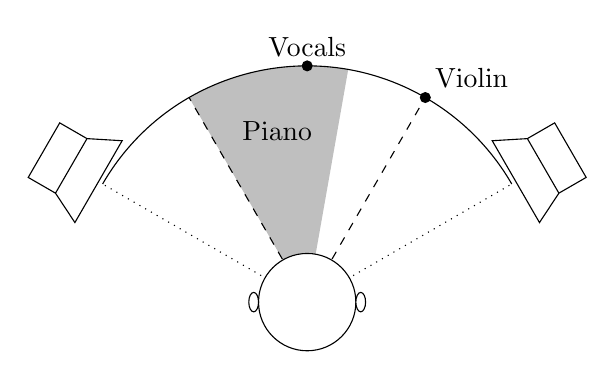
\begin{tikzpicture}
    \def\rad{3};
    \def\expand{1.02};

    \begin{scope}[rotate around={150:(0,0)}]
        \pic[transform shape, scale=0.2] (left_speaker) at (\rad*\expand,0) {speaker};
    \end{scope}

    \begin{scope}[rotate around={30:(0,0)}]
        \pic[transform shape, scale=0.2] (right_speaker) at (\rad*\expand,0) {speaker};
    \end{scope}

    % Piano
    \path[fill,lightgray] (0,0) -- (120:\rad)  arc (120:80:\rad) -- (0,0);
    \node at (100:2.2) {Piano};

    % Vocals
    \fill (0,0) (90:\rad) circle (2pt) node[above] {Vocals};

    % Violin
    \fill (0,0) (60:\rad) circle (2pt) node[above right] {Violin};

    % Stereo image
    \path[draw, dashed] (0,0) -- (120:\rad);
    \path[draw, dashed] (0,0) -- (60:\rad);
    \path[draw, dotted] (0,0) -- (150:\rad);
    \path[draw, dotted] (0,0) -- (30:\rad);

    % Draw full stereo image arc
    \draw (150:\rad) arc (150:30:\rad);

    % Music producer
    \pic[scale=0.618] (producer) at (0,0) {head};

\end{tikzpicture}
      \label{fig:stereo_image}
    \end{figure}
    \note{Refer to the thesis for logical explanation of how a stereo image is created}
  }

  \only<2-3> {
    \begin{columns}[b]
      \tiny
      \column{0.45\textwidth}
        \blockcquote[{Dave Pensado, Mixing Engineer, quoted in}][]{owsinskiMixingEngineersHandbook2006}{\revealedhl<3>{I think} that there are three sacred territories in a mix that if you put something there, you've got to have an incredibly good reason. That's extreme left, center, and extreme right. \revealedhl<3>{I've noticed} that \revealedhl<3>{some} mixers will get stereo tracks from synthesizers and effects, and they {just instinctively} pan them hard left and hard right. What they end up with is these \revealedhl<3>{big train wrecks} out on the ends of the stereo spectrum. Then they pan their kick, snare, bass, and vocals center, and you've got \revealedhl<3>{all this stuff} stacked on top of each other. If it were a visual, you wouldn't be able to see \revealedhl<3>{the things behind the things} in front. So \revealedhl<3>{what I do} is take a stereo synthesizer track, and \revealedhl<3>{I'll just toss} one side because I don't need it. I'll create my own stereo by either adding a delay or a chorus or a predelayed reverb or \revealedhl<3>{something like that} to give it a stereo image. I'll pan \revealedhl<3>{maybe} the dry signal to 10:00, and then I'll pan the effects just inside the extreme left side. \revealedhl<3>{I would never} put it hard left, because then \revealedhl<3>{there's too many things} on top of it. I would pan it at 9:00 and then pan the dry signal to \revealedhl<3>{say} 10:30, \revealedhl<3>{something like that}.}
        \vfill
      \column{0.45\textwidth}
        \blockcquote[{Steve Albini, Recording Engineer, quoted in}][]{owsinskiRecordingEngineersHandbook2009}{\revealedhl<3>{I've had really good luck} with the Neumann SM 2 stereo mic over the piano. AKG C 12s and C 24s \revealedhl<3>{sound great}, too. Those Audio-Technica 4051s are great piano mics. I'll \revealedhl<3>{usually} place them perpendicular to the harp, one on the long strings and one on the short strings. \revealedhl<3>{You have to shuffle them in and out until the stereo image sounds normal}. The SM 2 \revealedhl<3>{I'll put in front} of the piano with the lid open, \revealedhl<3>{sort of} looking in on the strings. Same with the C 24.}
        \vfill
    \end{columns}
  }
  \note{Don't spend too much effort reading these quotes, but they are from music profesionals at the top of their game, and their explanation of how they create stereo field is essentially "I dunno, I just do what sounds good".}

\end{frame}

\begin{frame}
  \frametitle{What is... \ftfill{} {\tiny Analysis of stereo image in vast repositories of} recorded music ?}
  \socrates
  \begin{block}{recorded...}
    \begin{itemize}
      \item Digital audio recordings
      \item Available for analysis
    \end{itemize}
  \end{block}
  \begin{block}{...music}
    \begin{itemize}
      \item No-one can agree \parencite{cobussenDeconstructionMusic2002}
      \item Ask the creator
    \end{itemize}
  \end{block}
\end{frame}

\begin{frame}
  \frametitle{What is... \ftfill{} {\tiny Analysis of stereo image in} vast {\tiny repositories of recorded music} ?}
  \socrates
  \centering
  \begin{tikzpicture}
    \node [thick, draw=black, inner sep=0pt, copy shadow={draw=gray, fill=gray, shadow xshift=0.5em, shadow yshift=-0.5em}] { 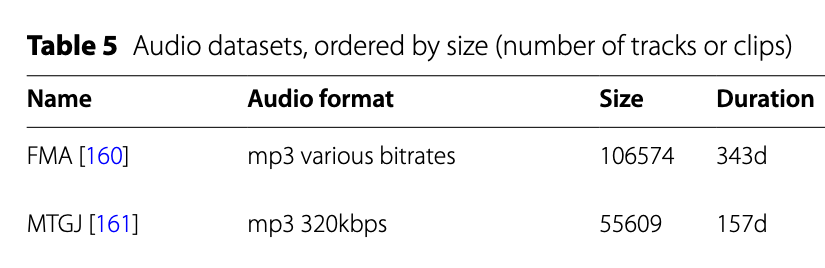
\includegraphics[width=0.618\linewidth]{what_is_vast.png} };
  \end{tikzpicture}

  \vspace{3mm}
  \parencite{miticSystematicLiteratureReview2026}
\end{frame}

\subsection{How recordings happen}
\subsectionslide

\begin{frame}
  \frametitle{Recording Studios}
  \centering
  \only<1>{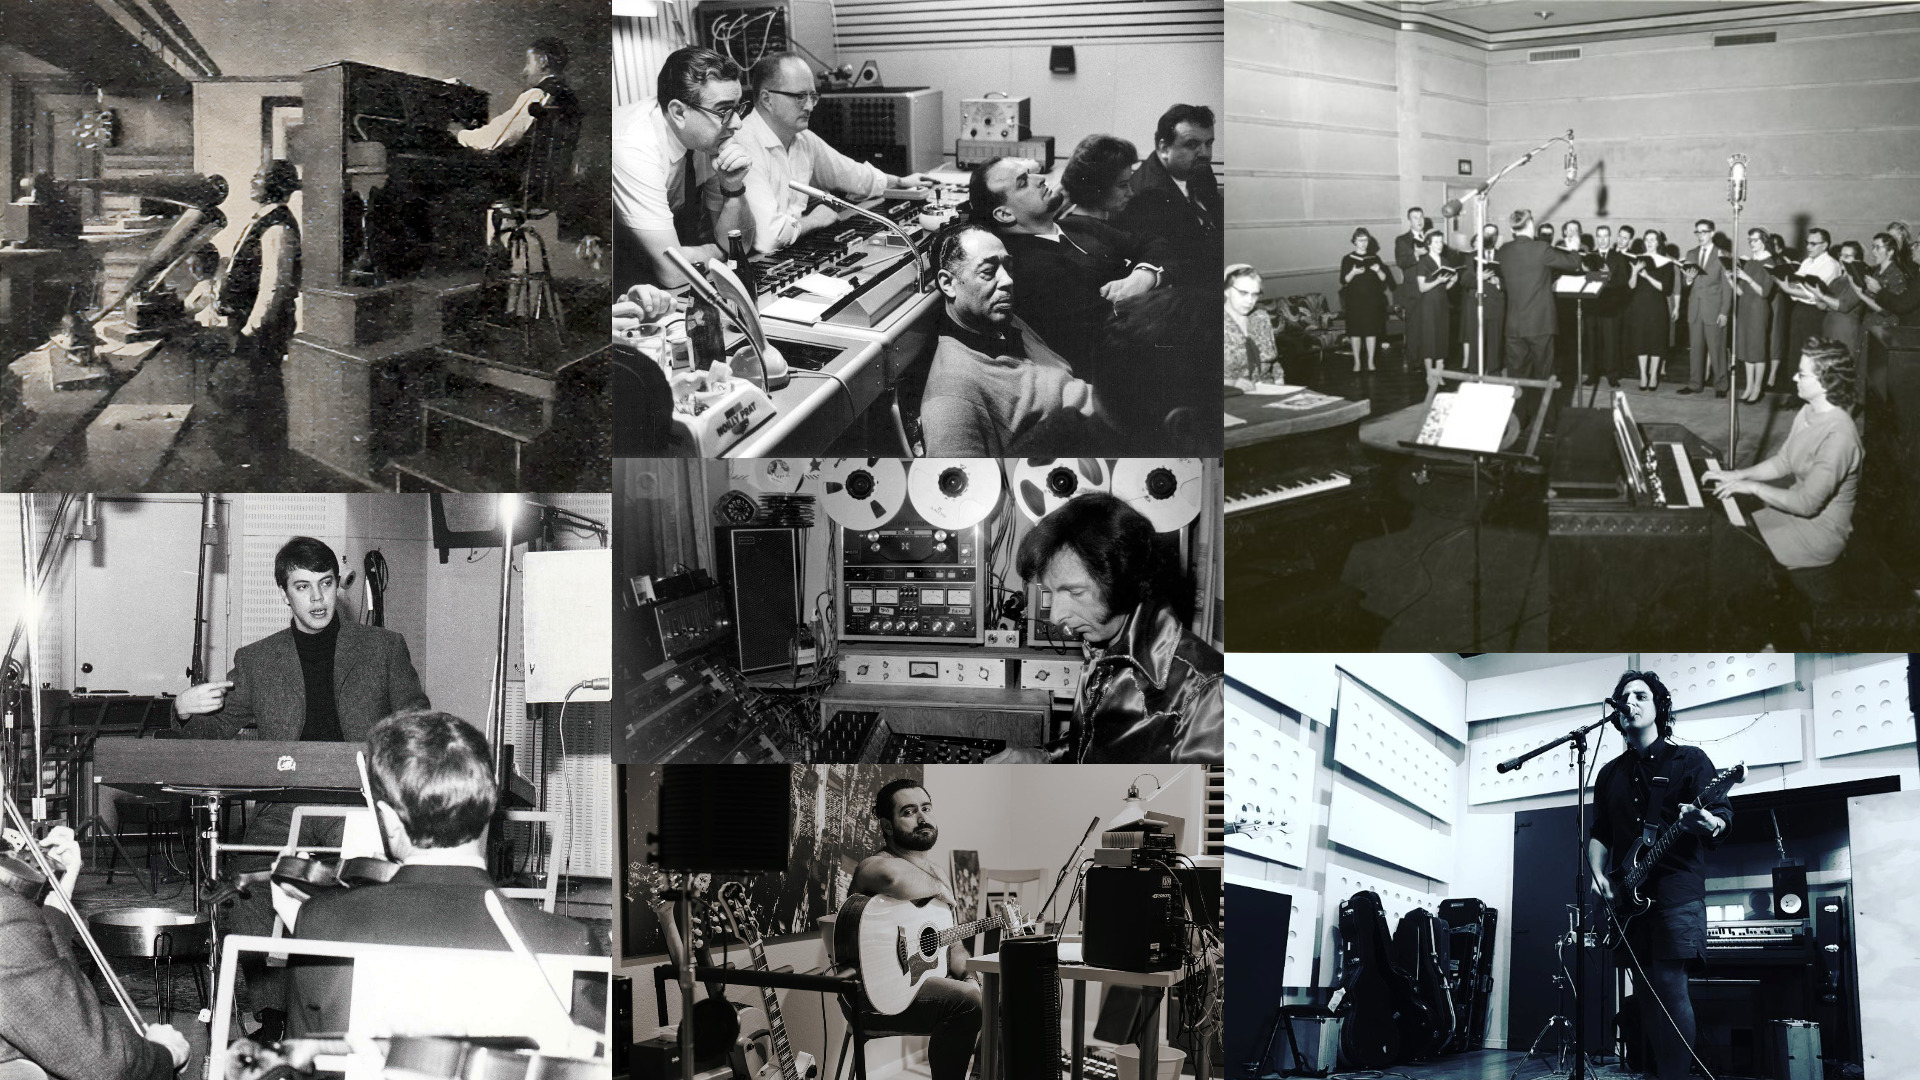
\includegraphics[width=\linewidth]{img/gandr-collage_1.jpg}}
  \only<2>{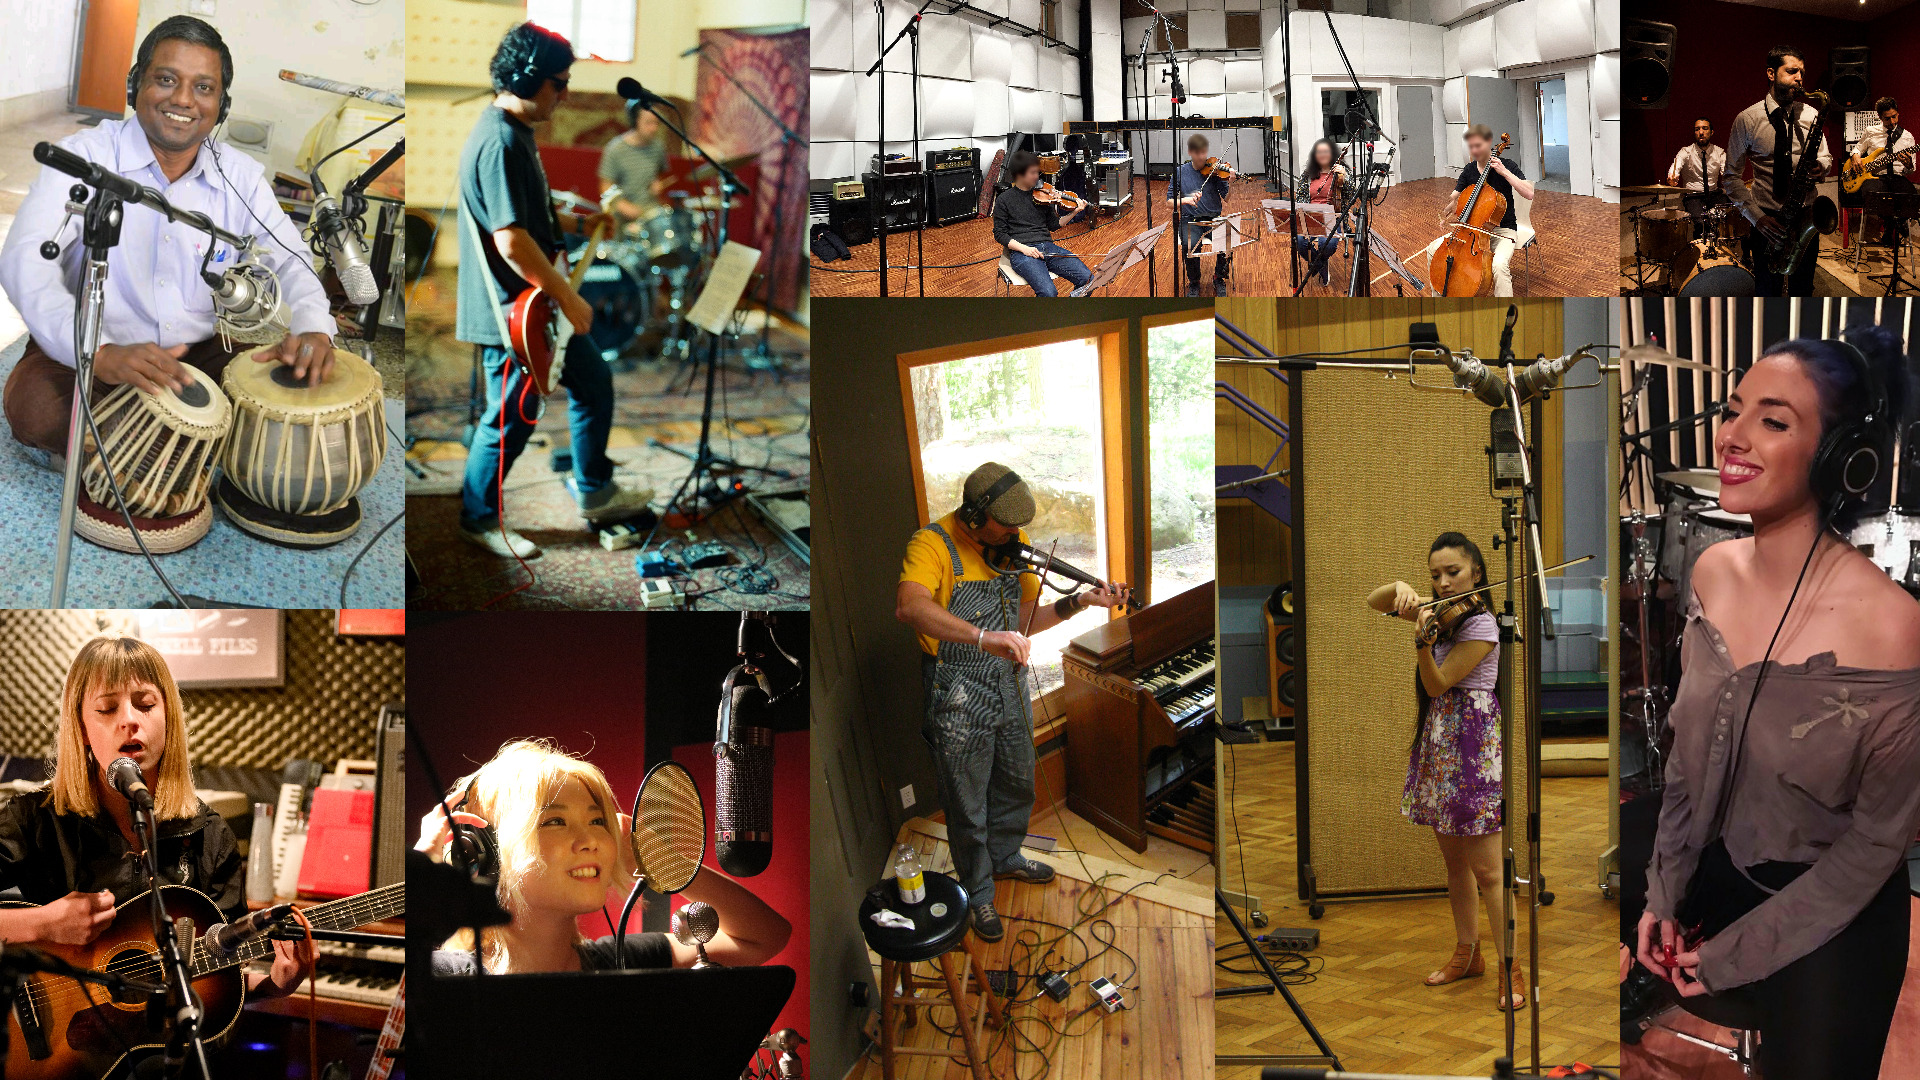
\includegraphics[width=\linewidth]{img/gandr-collage_2.jpg}}
  \only<3>{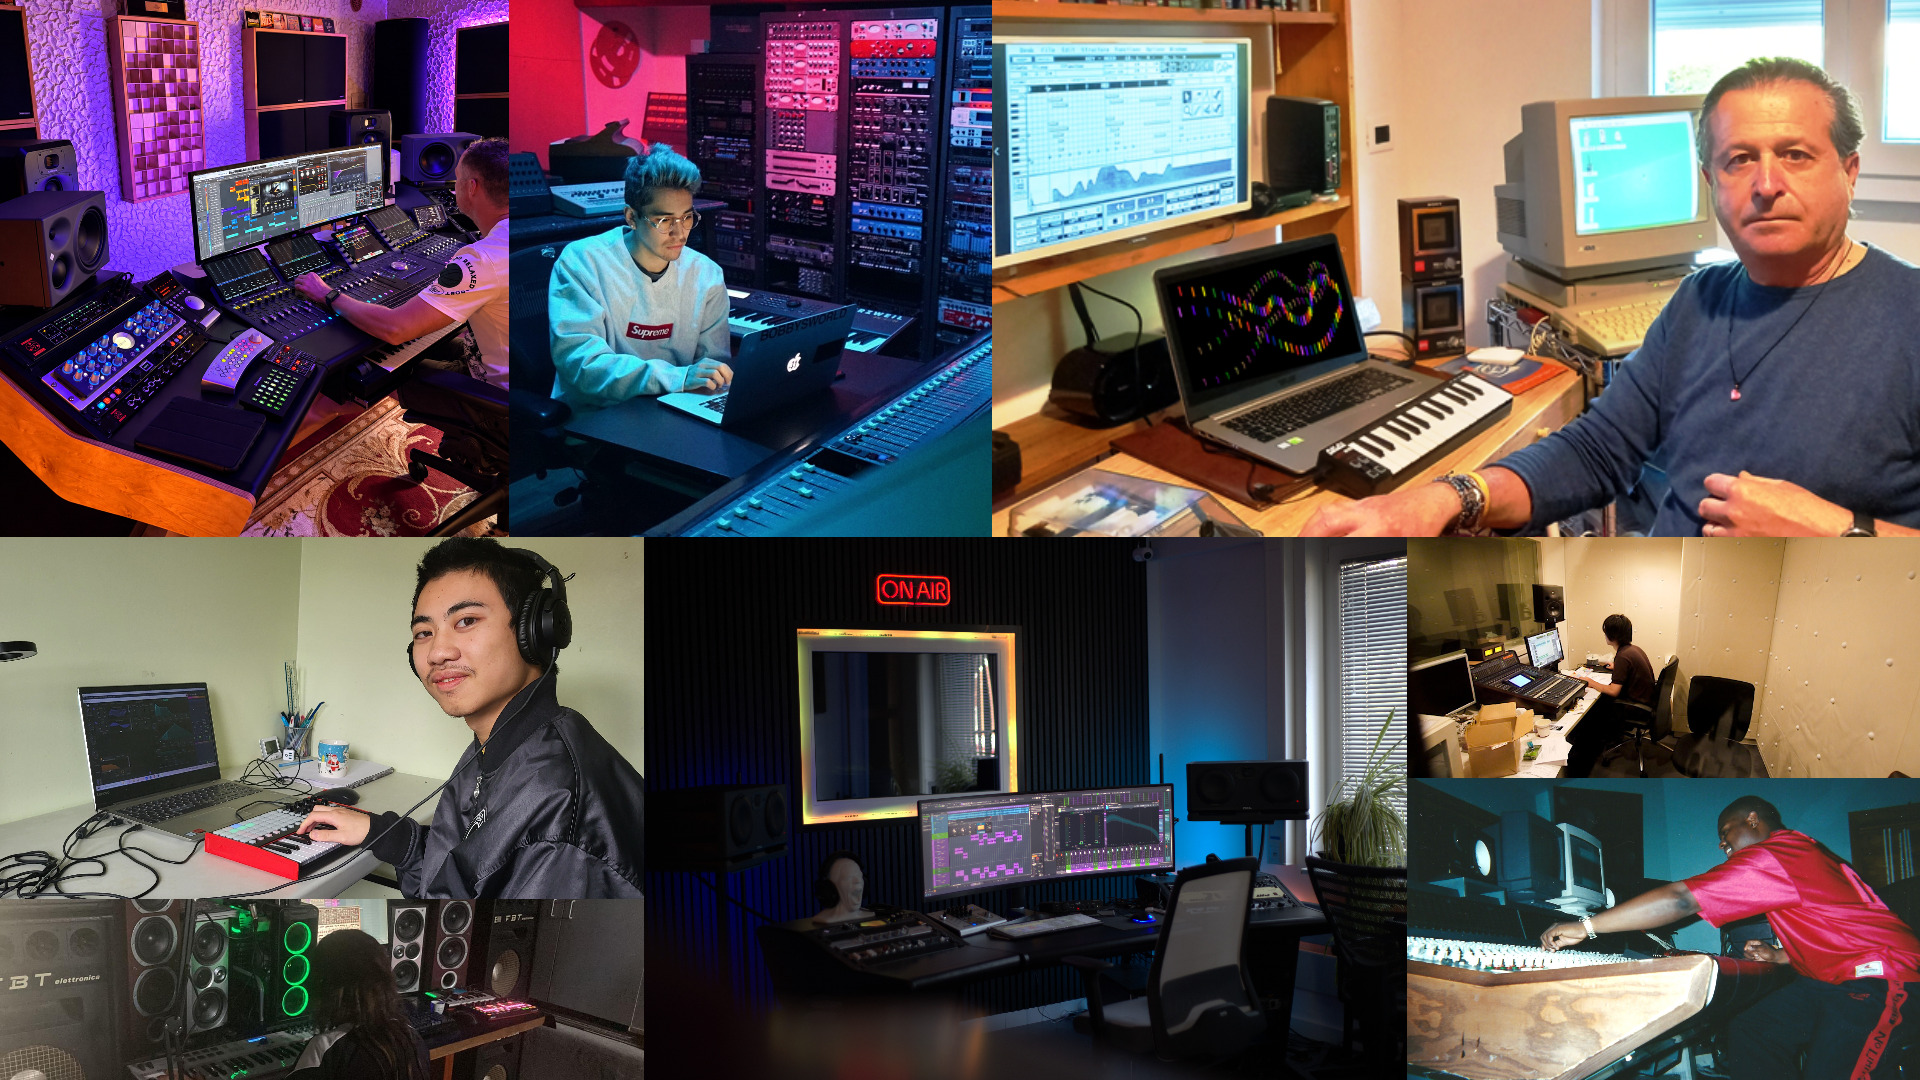
\includegraphics[width=\linewidth]{img/gandr-collage_3.jpg}}
  \only<4>{
    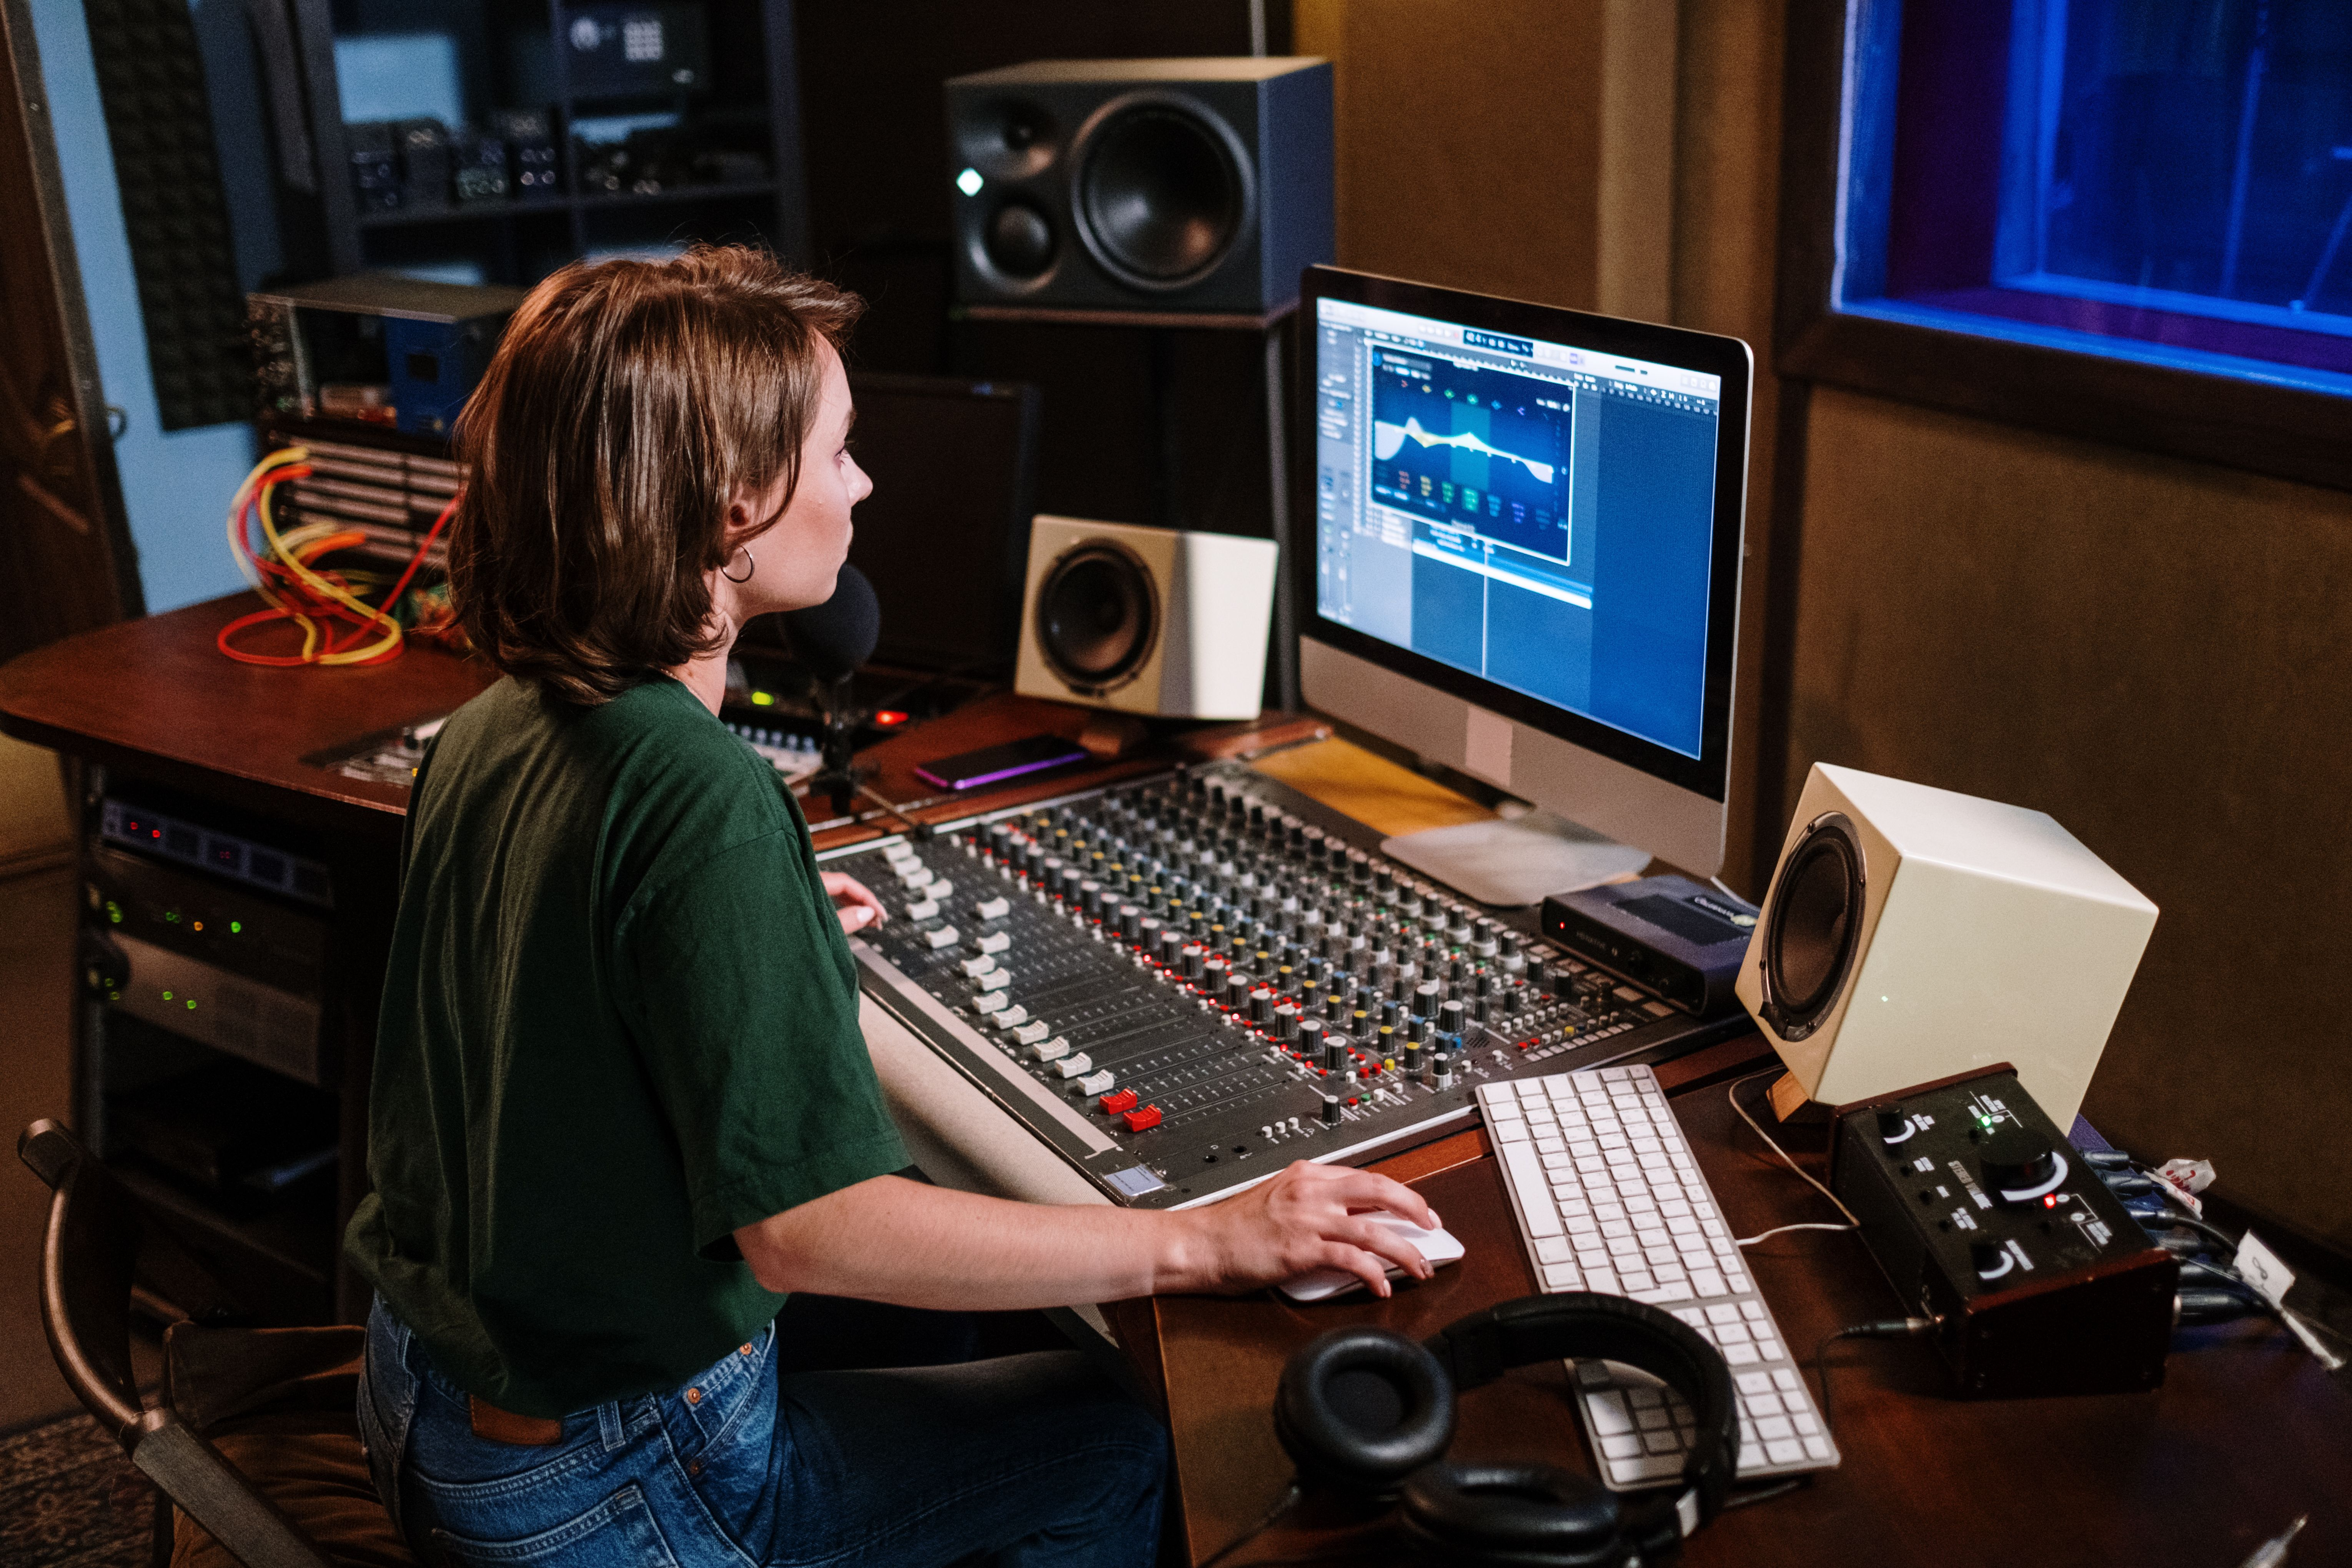
\includegraphics[height=0.67\textheight]{img/pexels-cottonbro-5657670.jpg}
    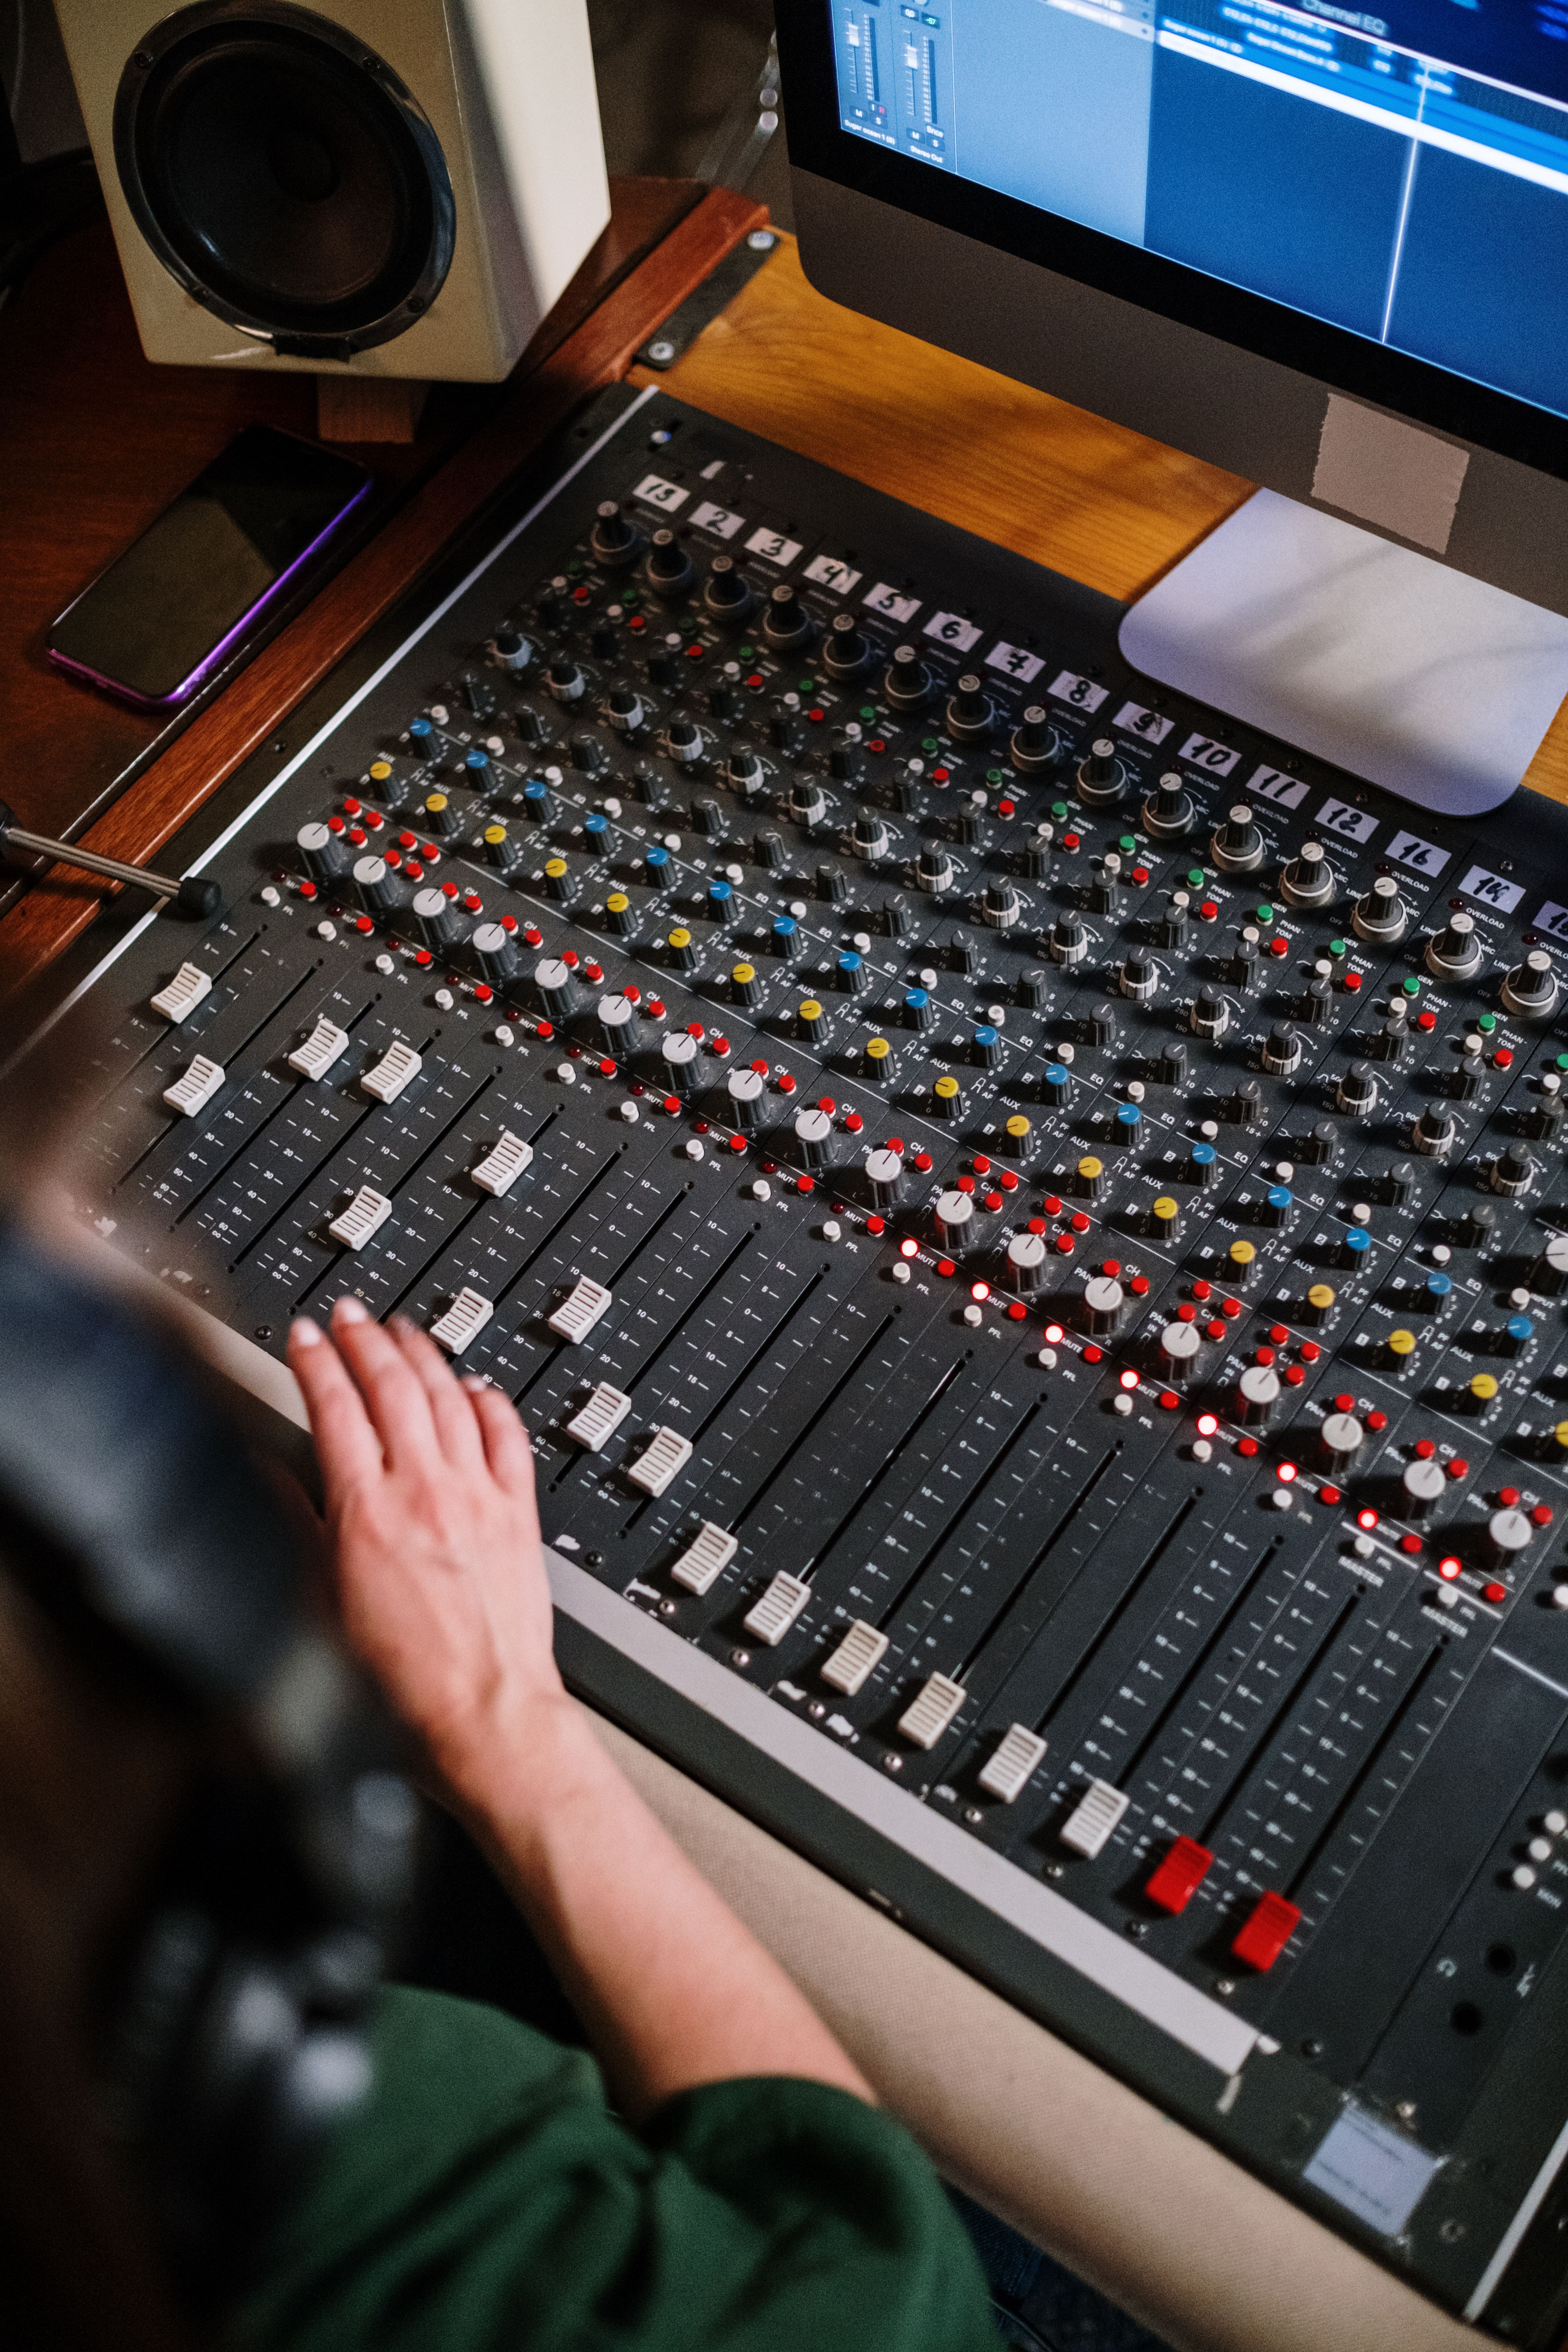
\includegraphics[height=0.67\textheight]{img/pexels-cottonbro-5657676.jpg}
  }
\end{frame}

\begin{frame}
  \frametitle{Digital Audio Workstation}
  \centering
  \def\pluginwidth{3.2cm}
  \begin{tikzpicture}
    \node[anchor=north west] (daw) at (0,0) {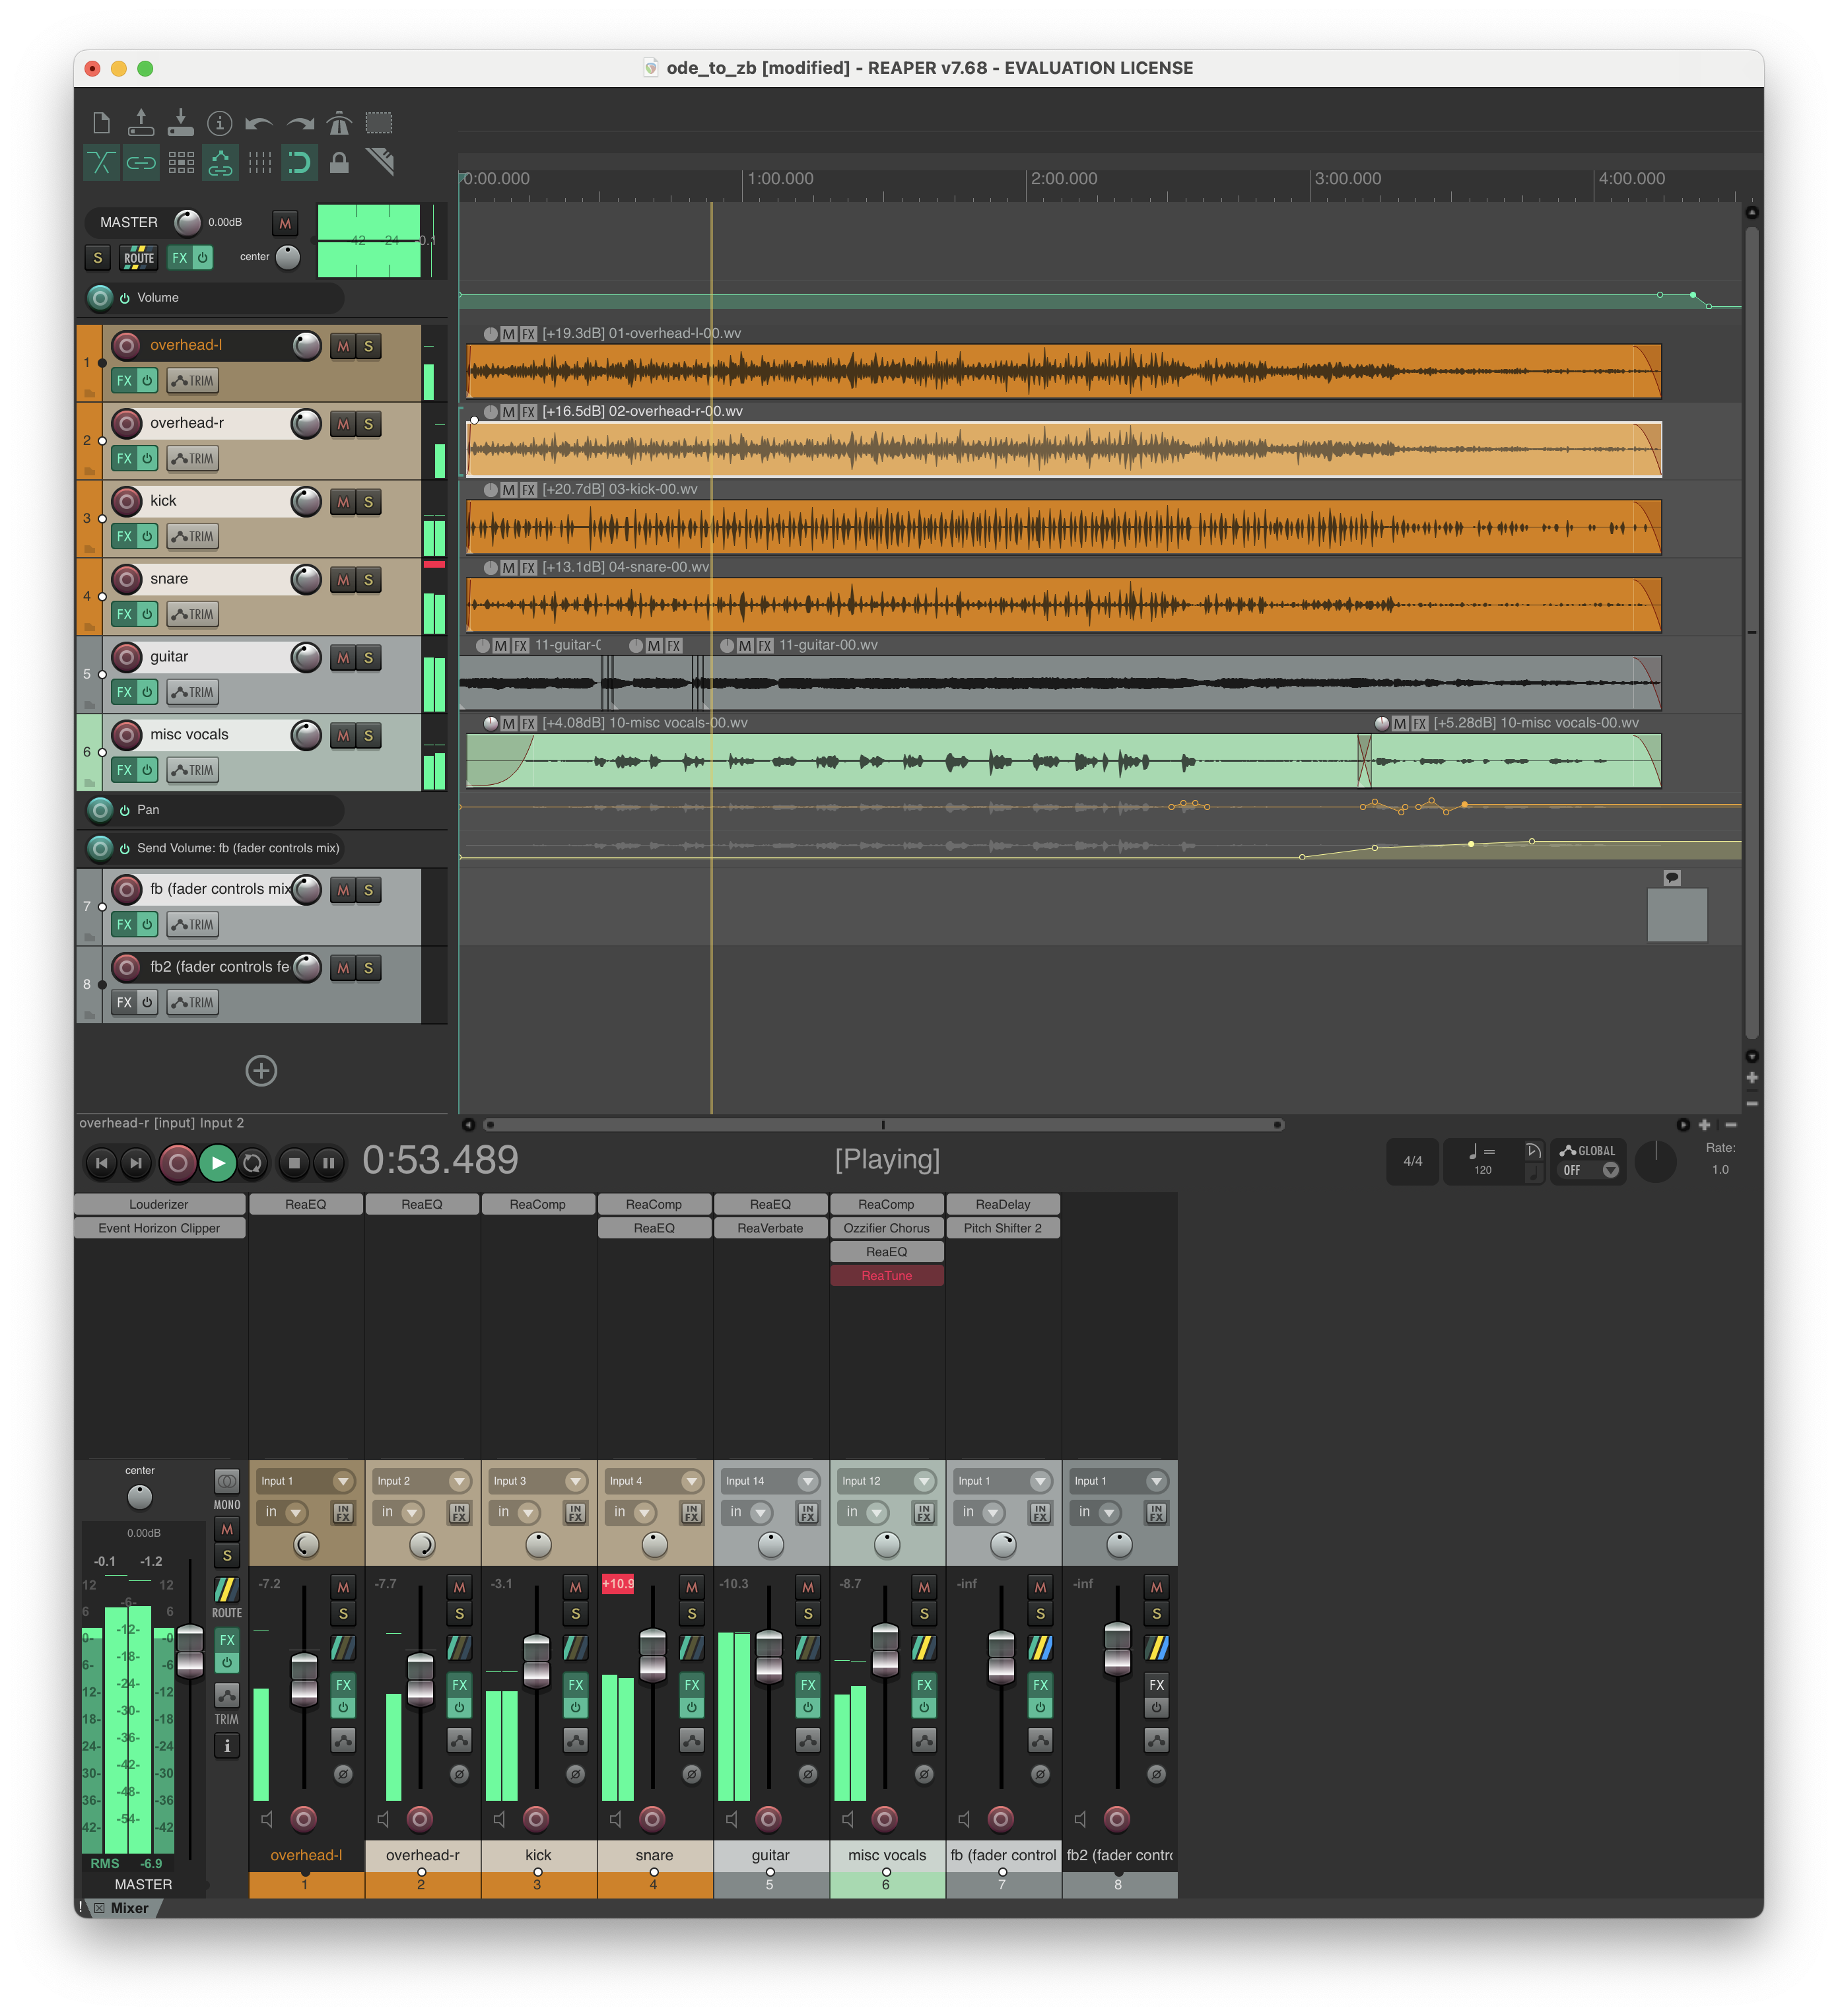
\includegraphics[height=0.8\textheight]{odetozb.png}};
    \node[anchor=north west] (eq) at (daw.north east) {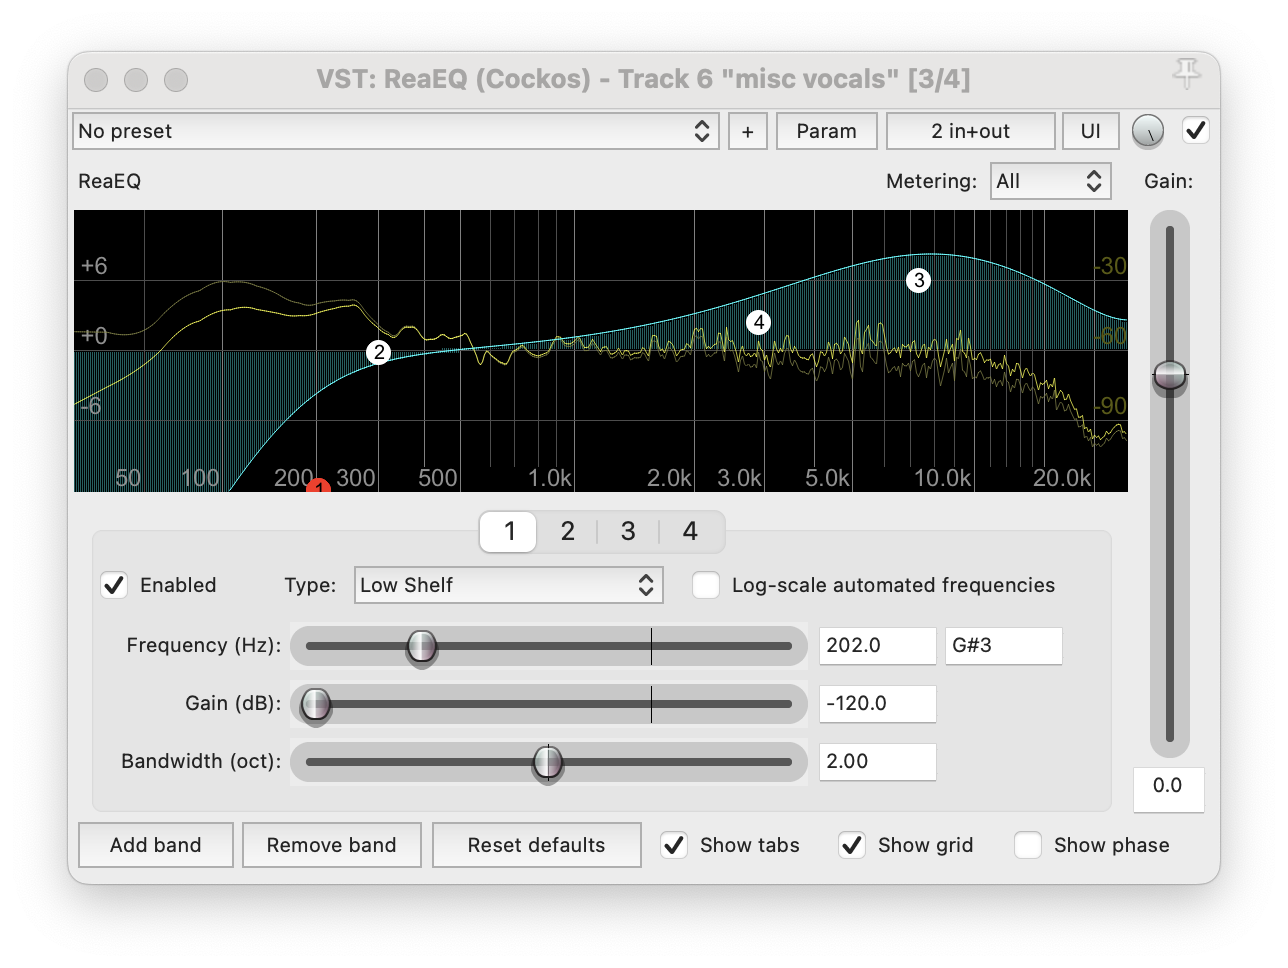
\includegraphics[width=\pluginwidth]{eq.png}};
    \node[anchor=west] (eq) at ($(daw.east) + (0,0.35)$) {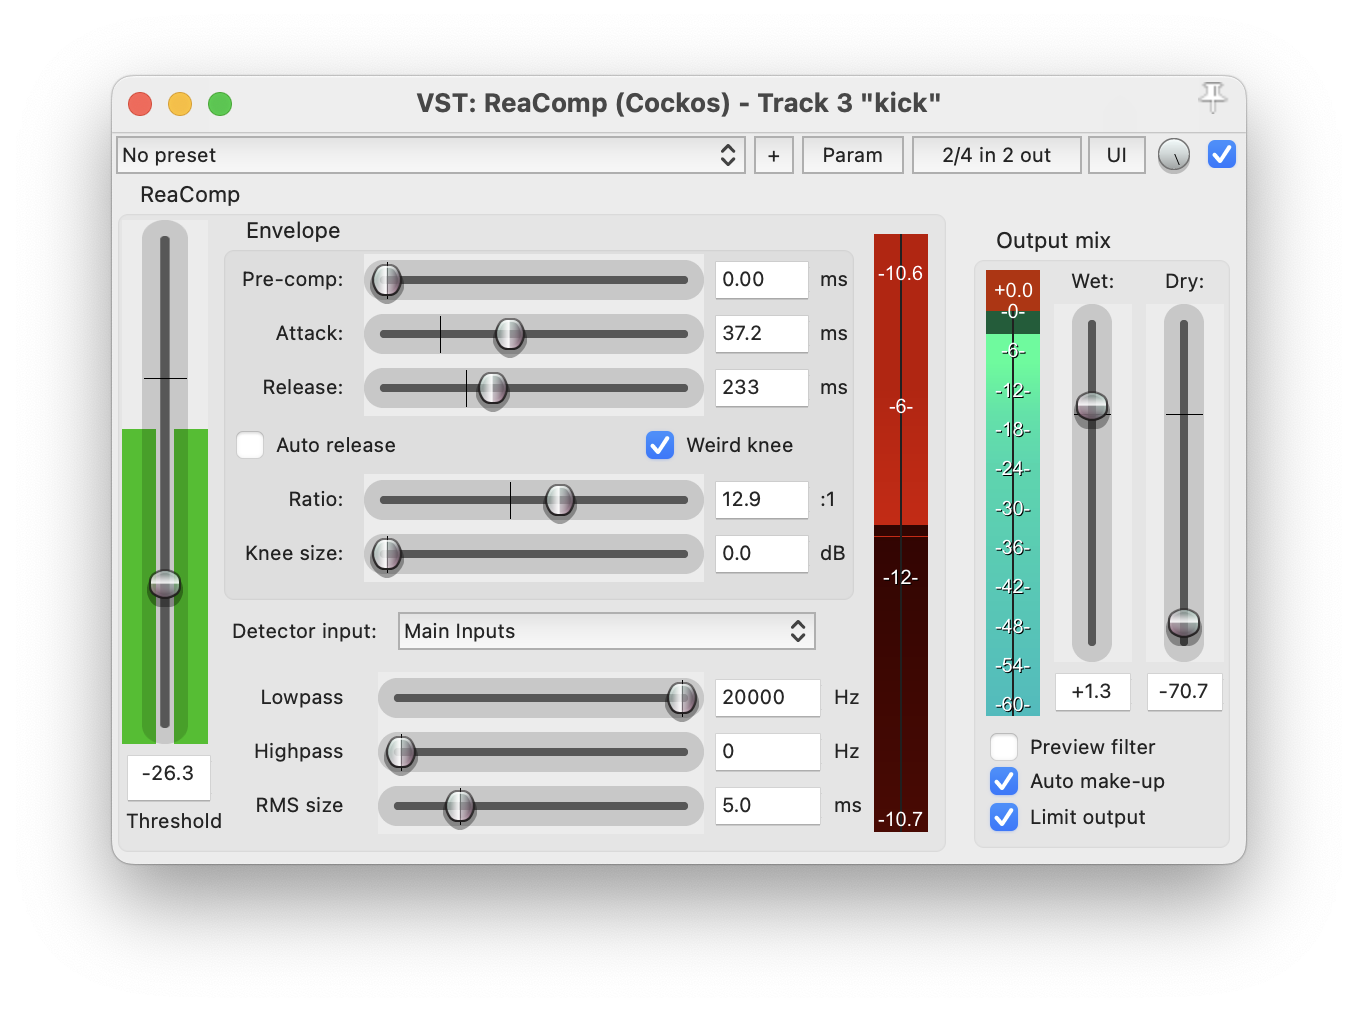
\includegraphics[width=\pluginwidth]{compressor.png}};
    \node[anchor=south west] (eq) at (daw.south east) {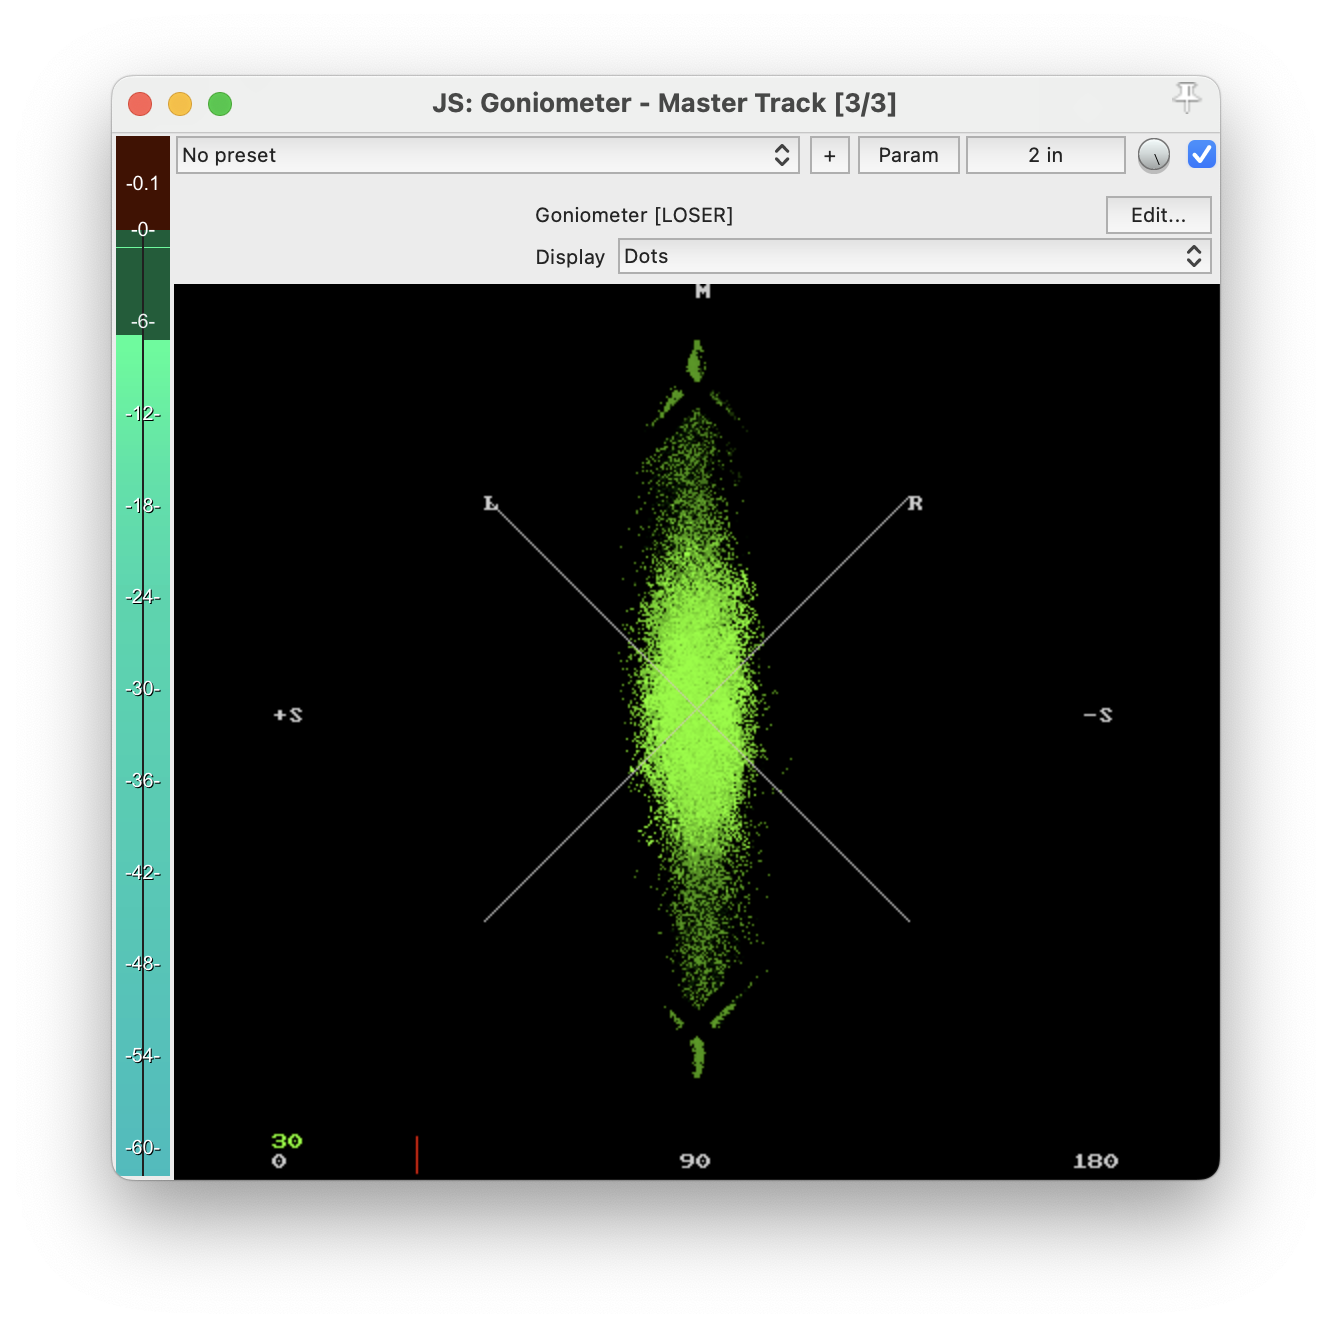
\includegraphics[width=\pluginwidth]{goniometer.png}};
  \end{tikzpicture}
  \footnote{\url{https://www.cockos.com/reaper/samples/ode_to_zb.zip}}
\end{frame}

\begin{frame}
  \frametitle{Distribution}
  \begin{itemize}
    \item Producer renders a mixdown
    \item Mastering engineer makes a master
    \item Master is sent to distributor(s)
    \item Distributor(s) make(s) several encodings
    \item Encodings are played by a listener
    \begin{itemize}
      \item \alert{$\uparrow$ This is the recording available for analysis}
    \end{itemize}
  \end{itemize}
\end{frame}


\section{Research}

\subsection{Motivation}

\subsectionslide

\begin{frame}
  \frametitle{Motivation}
  \begin{itemize}
    \setlength{\itemsep}{6pt}
    \item The amount of available recorded music has skyrocketed
    \item Every track represents a combination of artistic choices
    \item It's an opportunity to learn about human creativity
  \end{itemize}
\end{frame}

\begin{frame}
  \frametitle{Datasets}
  \begin{block}{Public}
    \begin{itemize}
      \item Free Music Archive - \cite{defferrardFMADatasetMusic2017}
      \item MTG Jamendo - \cite{bogdanovMTGJamendoDatasetAutomatic2019}
      \item More smaller...
    \end{itemize}
  \end{block}
  \begin{block}{Private}
    \begin{columns}[T]
      \column{0.48\textwidth}
        \begin{itemize}
          \item Personal collections 
          \begin{itemize}
            \item \cite{tzanetakisStereoPanningFeatures2007}
            \item \cite{tardieuProductionEffectAudio2011}
            \item \cite{yangUpmixingStyleTransfer2022}
            \item \cite{ziemerProducerVsRapper2025}
          \end{itemize}
        \end{itemize}
      \column{0.48\textwidth}
        \begin{itemize}
        \item Company licensed
        \begin{itemize}
          \item \cite{bourbonInvestigationImmersiveContemporary2023}
          \item \cite{mourgelaExploringTrendsAudio2024}
        \end{itemize}
      \end{itemize}
    \end{columns}
  \end{block}
\end{frame}


\subsection{Research questions}
\subsectionslide

\begin{frame}
  \frametitle{Research Questions}
  \begin{block}{Overarching}
    How do music producers use stereo field?
  \end{block}
  \begin{block}{Sub questions}
    \begin{enumerate}[leftmargin=3em]
      \setlength{\itemsep}{6pt}
      \item[\rqone{}:] How does the stereo image of a recording relate to\\real-world musical knowledge? \label{rq:usecase}
      \item[\rqtwo{}:] What methods can be used to describe the\\stereo image of a music recording? \label{rq:methods}
    \end{enumerate}
  \end{block}
\end{frame}

\subsection{Methodology}
\subsectionslide

\begin{frame}
  \frametitle{A dual methodology}
  Two work-streams with different epistemologies

  \begin{block}{Constructive (\rqone{})}
    \begin{itemize}
      \item Immersion in musical practice
      \item Stereo field perception
      \item Understand what can be measured
    \end{itemize}
  \end{block}

  \begin{block}{Objective (\rqtwo{})}
    \begin{itemize}
      \item Systematic Literature Review
      \item Software for measurement of stereo image
    \end{itemize}
  \end{block}

\end{frame}

\begin{frame}
  \frametitle{A dual methodology (in reality)}
  \centering
  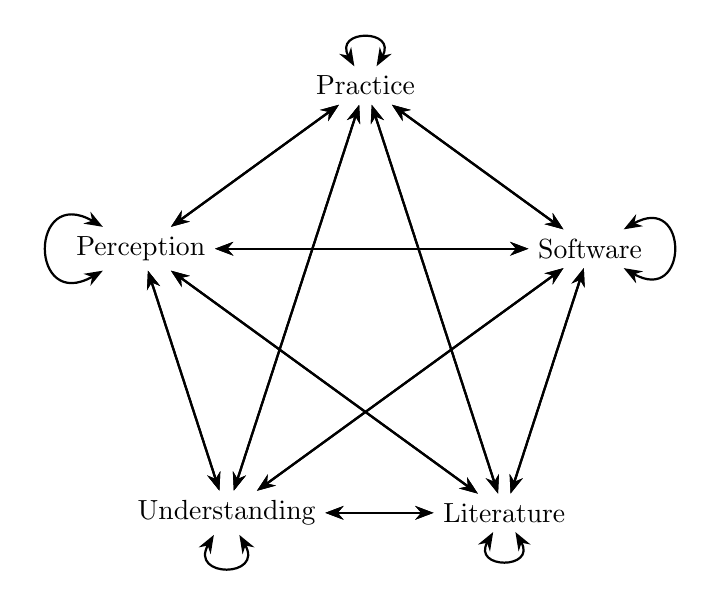
\begin{tikzpicture}[
    arrow/.style={
      Stealth-Stealth,
      thick,
      draw=black,
    },
   ]
    \def\r{3};
    % Peripheral Nodes arranged in a circle around the center
    \node (prac) at (90:\r)   {Practice};
    \node (perc) at (162:\r)  {Perception};
    \node (und)  at (234:\r)  {Understanding};
    \node (slr)  at (306:\r)  {Literature};
    \node (sw)   at (18:\r)   {Software};

    \foreach \a/\ang in {prac/90, perc/180, und/270, slr/270, sw/0} {
      \foreach \b in {prac, perc, und, slr, sw} {
        \ifthenelse{\NOT\equal{\a}{\b}}{\draw[arrow] (\a) -- (\b);}{}
      }
      \draw[arrow] (\a) edge [in=\ang-30, out=\ang+30, loop, looseness=5] (\a);
    }
  \end{tikzpicture}

\end{frame}

\begin{frame}[allowframebreaks]
  \frametitle{The Auxtrument}
  \begin{figure}
    \centering
    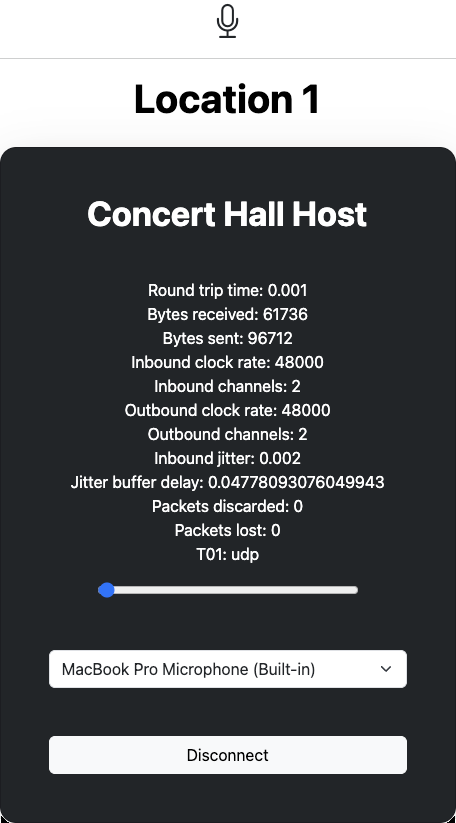
\includegraphics[height=0.55\textheight, keepaspectratio]{auxtrument_app.png} \quad
    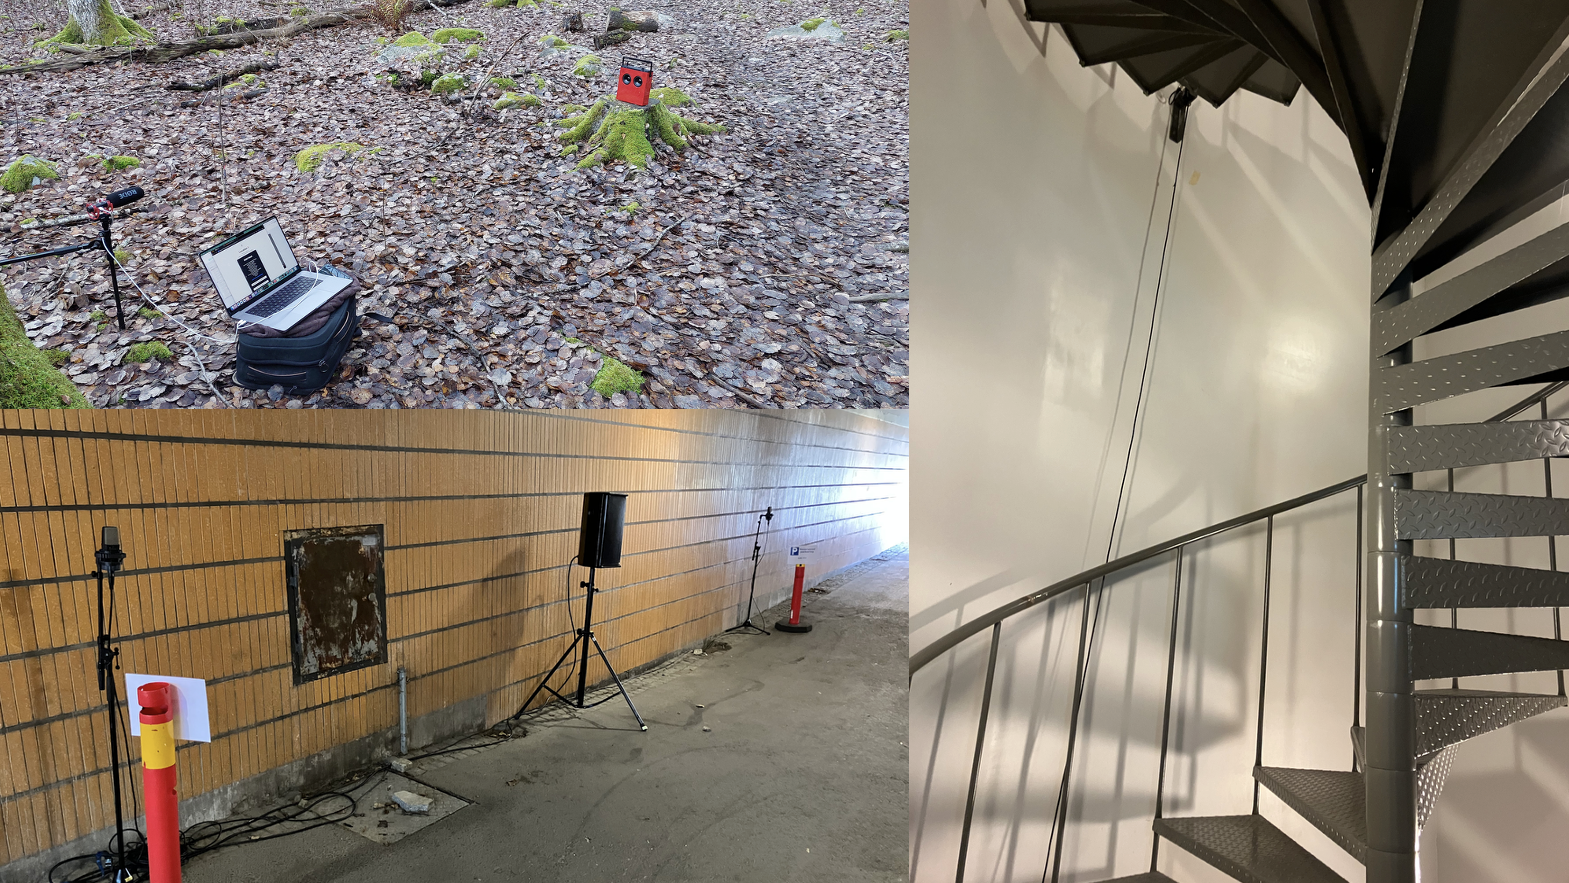
\includegraphics[height=0.55\textheight, keepaspectratio]{auxtrument_locations.png}
    \\\parencite{franklinComposingNetworkedReverberation2025}
  \end{figure}

  \begin{figure}
    \centering
    \begin{tikzpicture}
      \node[anchor=north west] (pic1) at (0,0) {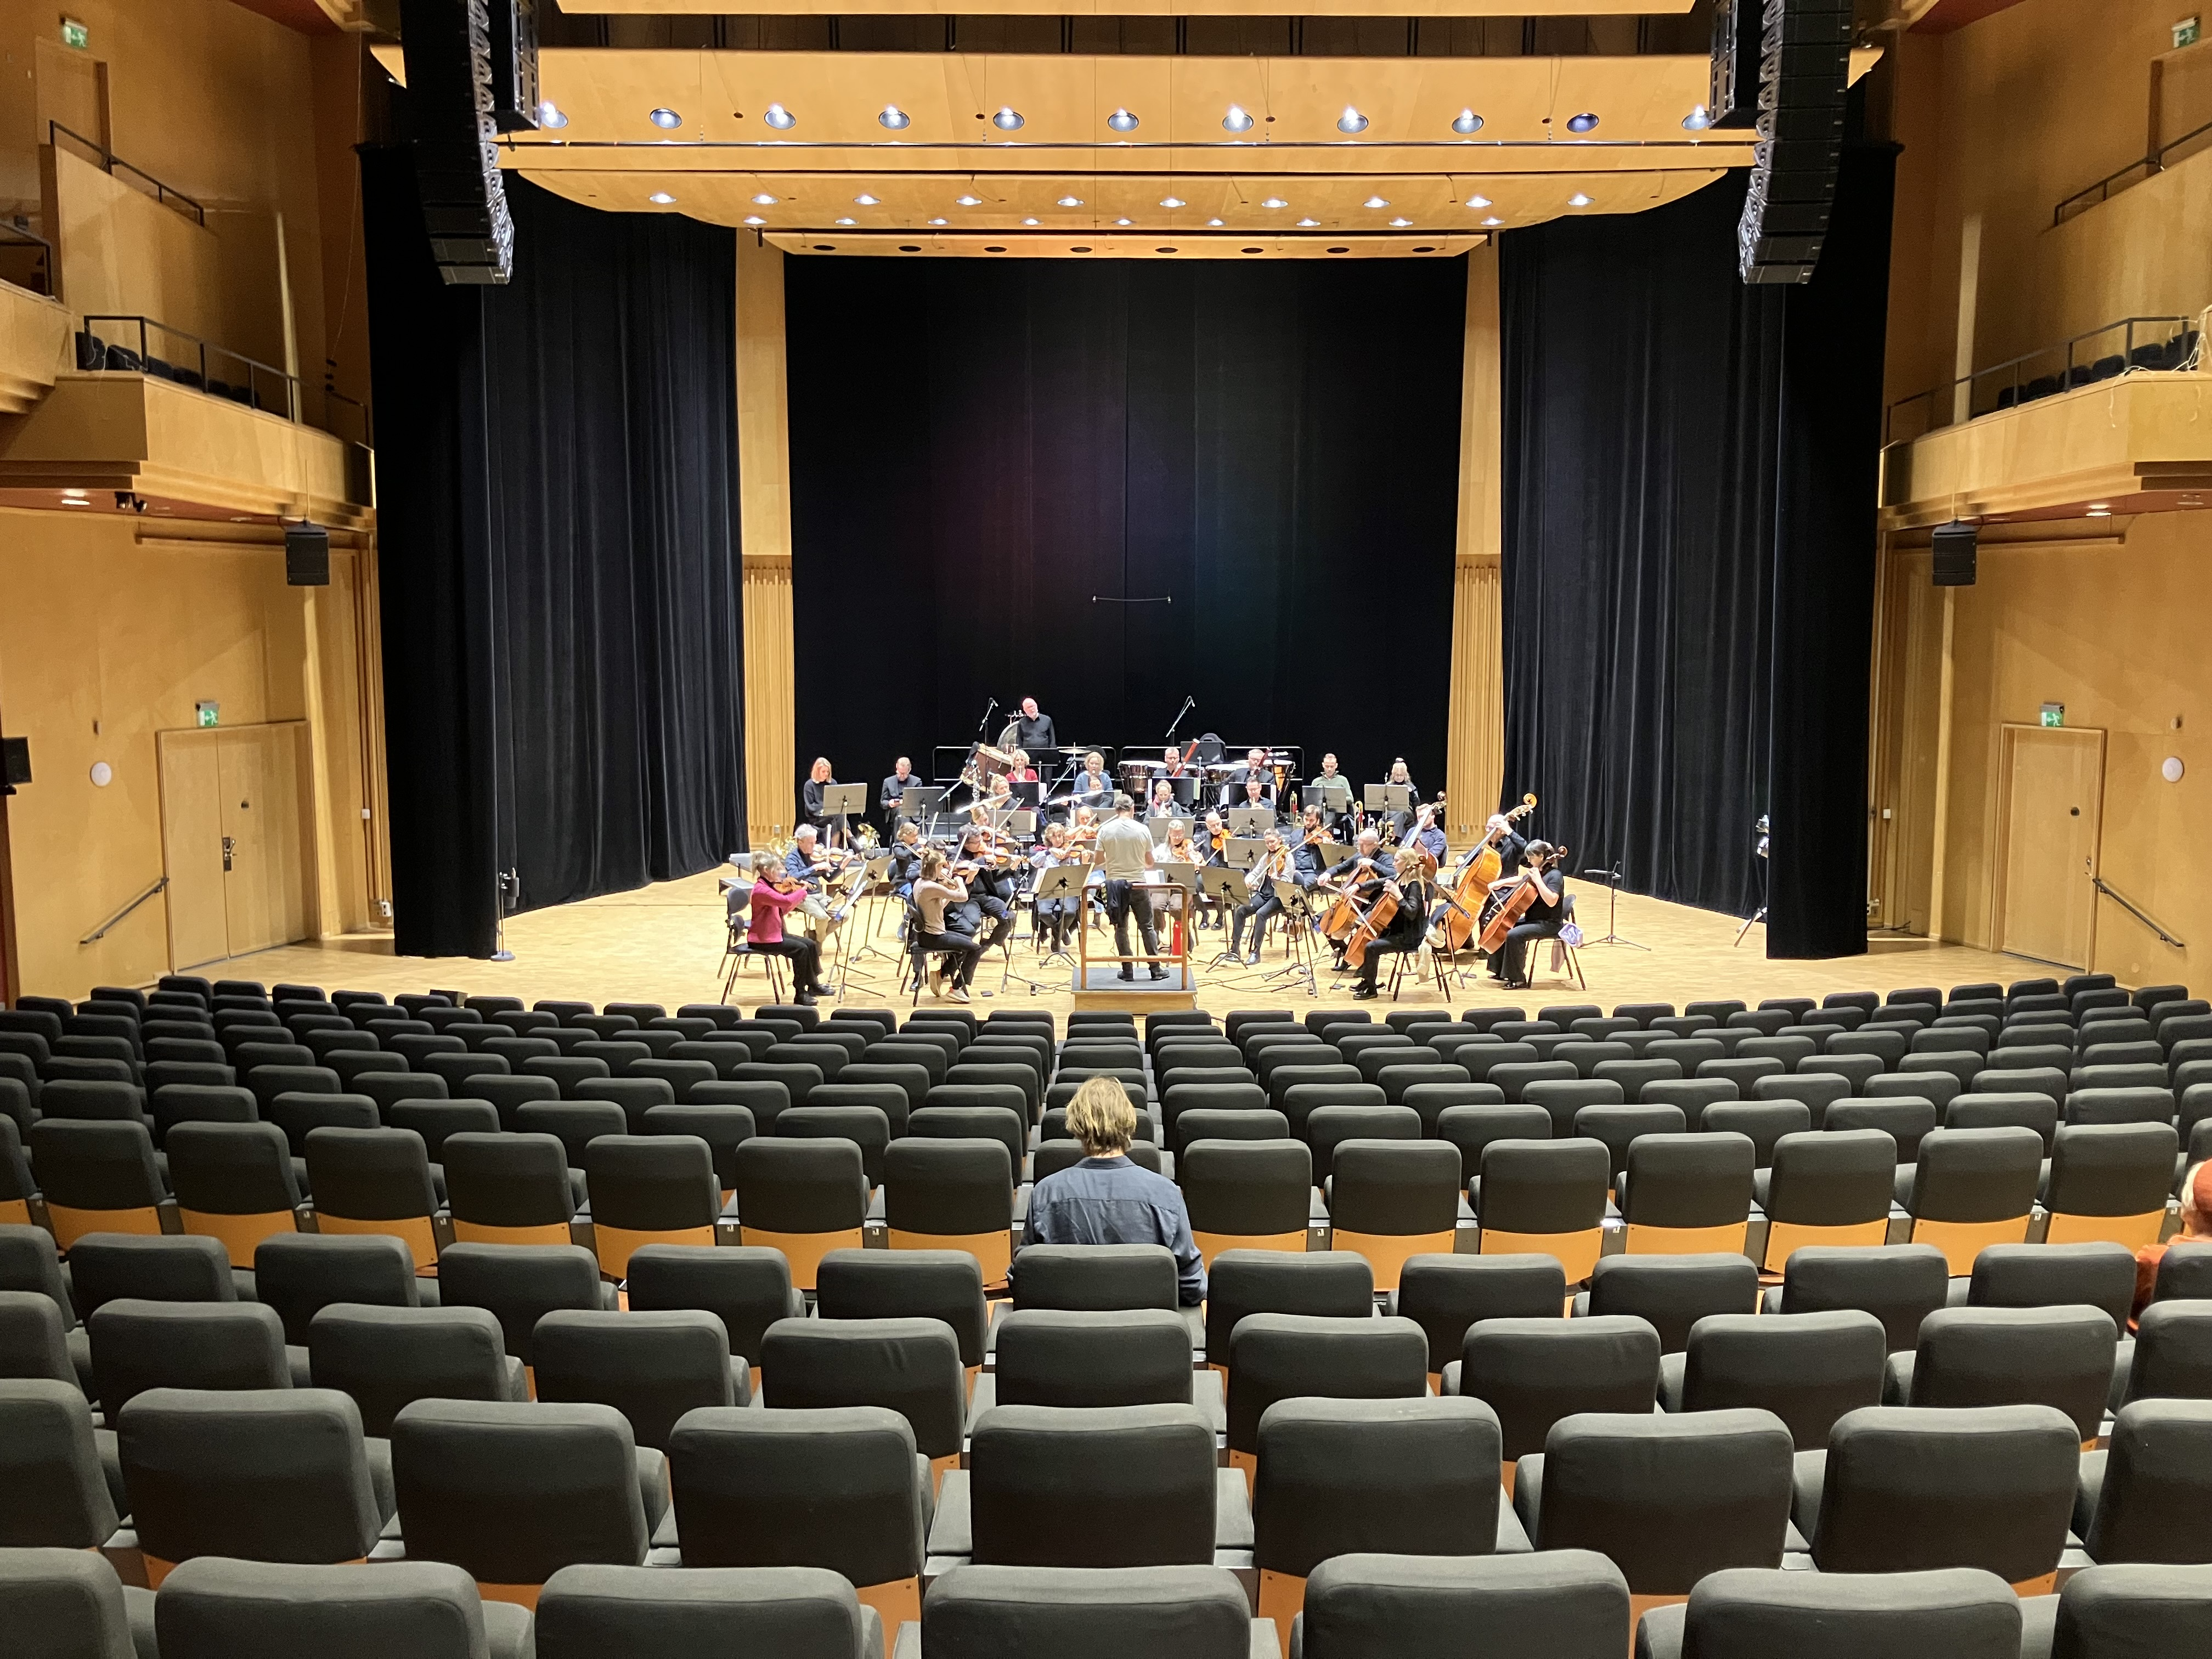
\includegraphics[width=6.5cm, keepaspectratio]{img/IMG_0994.jpg}};
      \node[anchor=north west] (pic2) at (6.5,0) {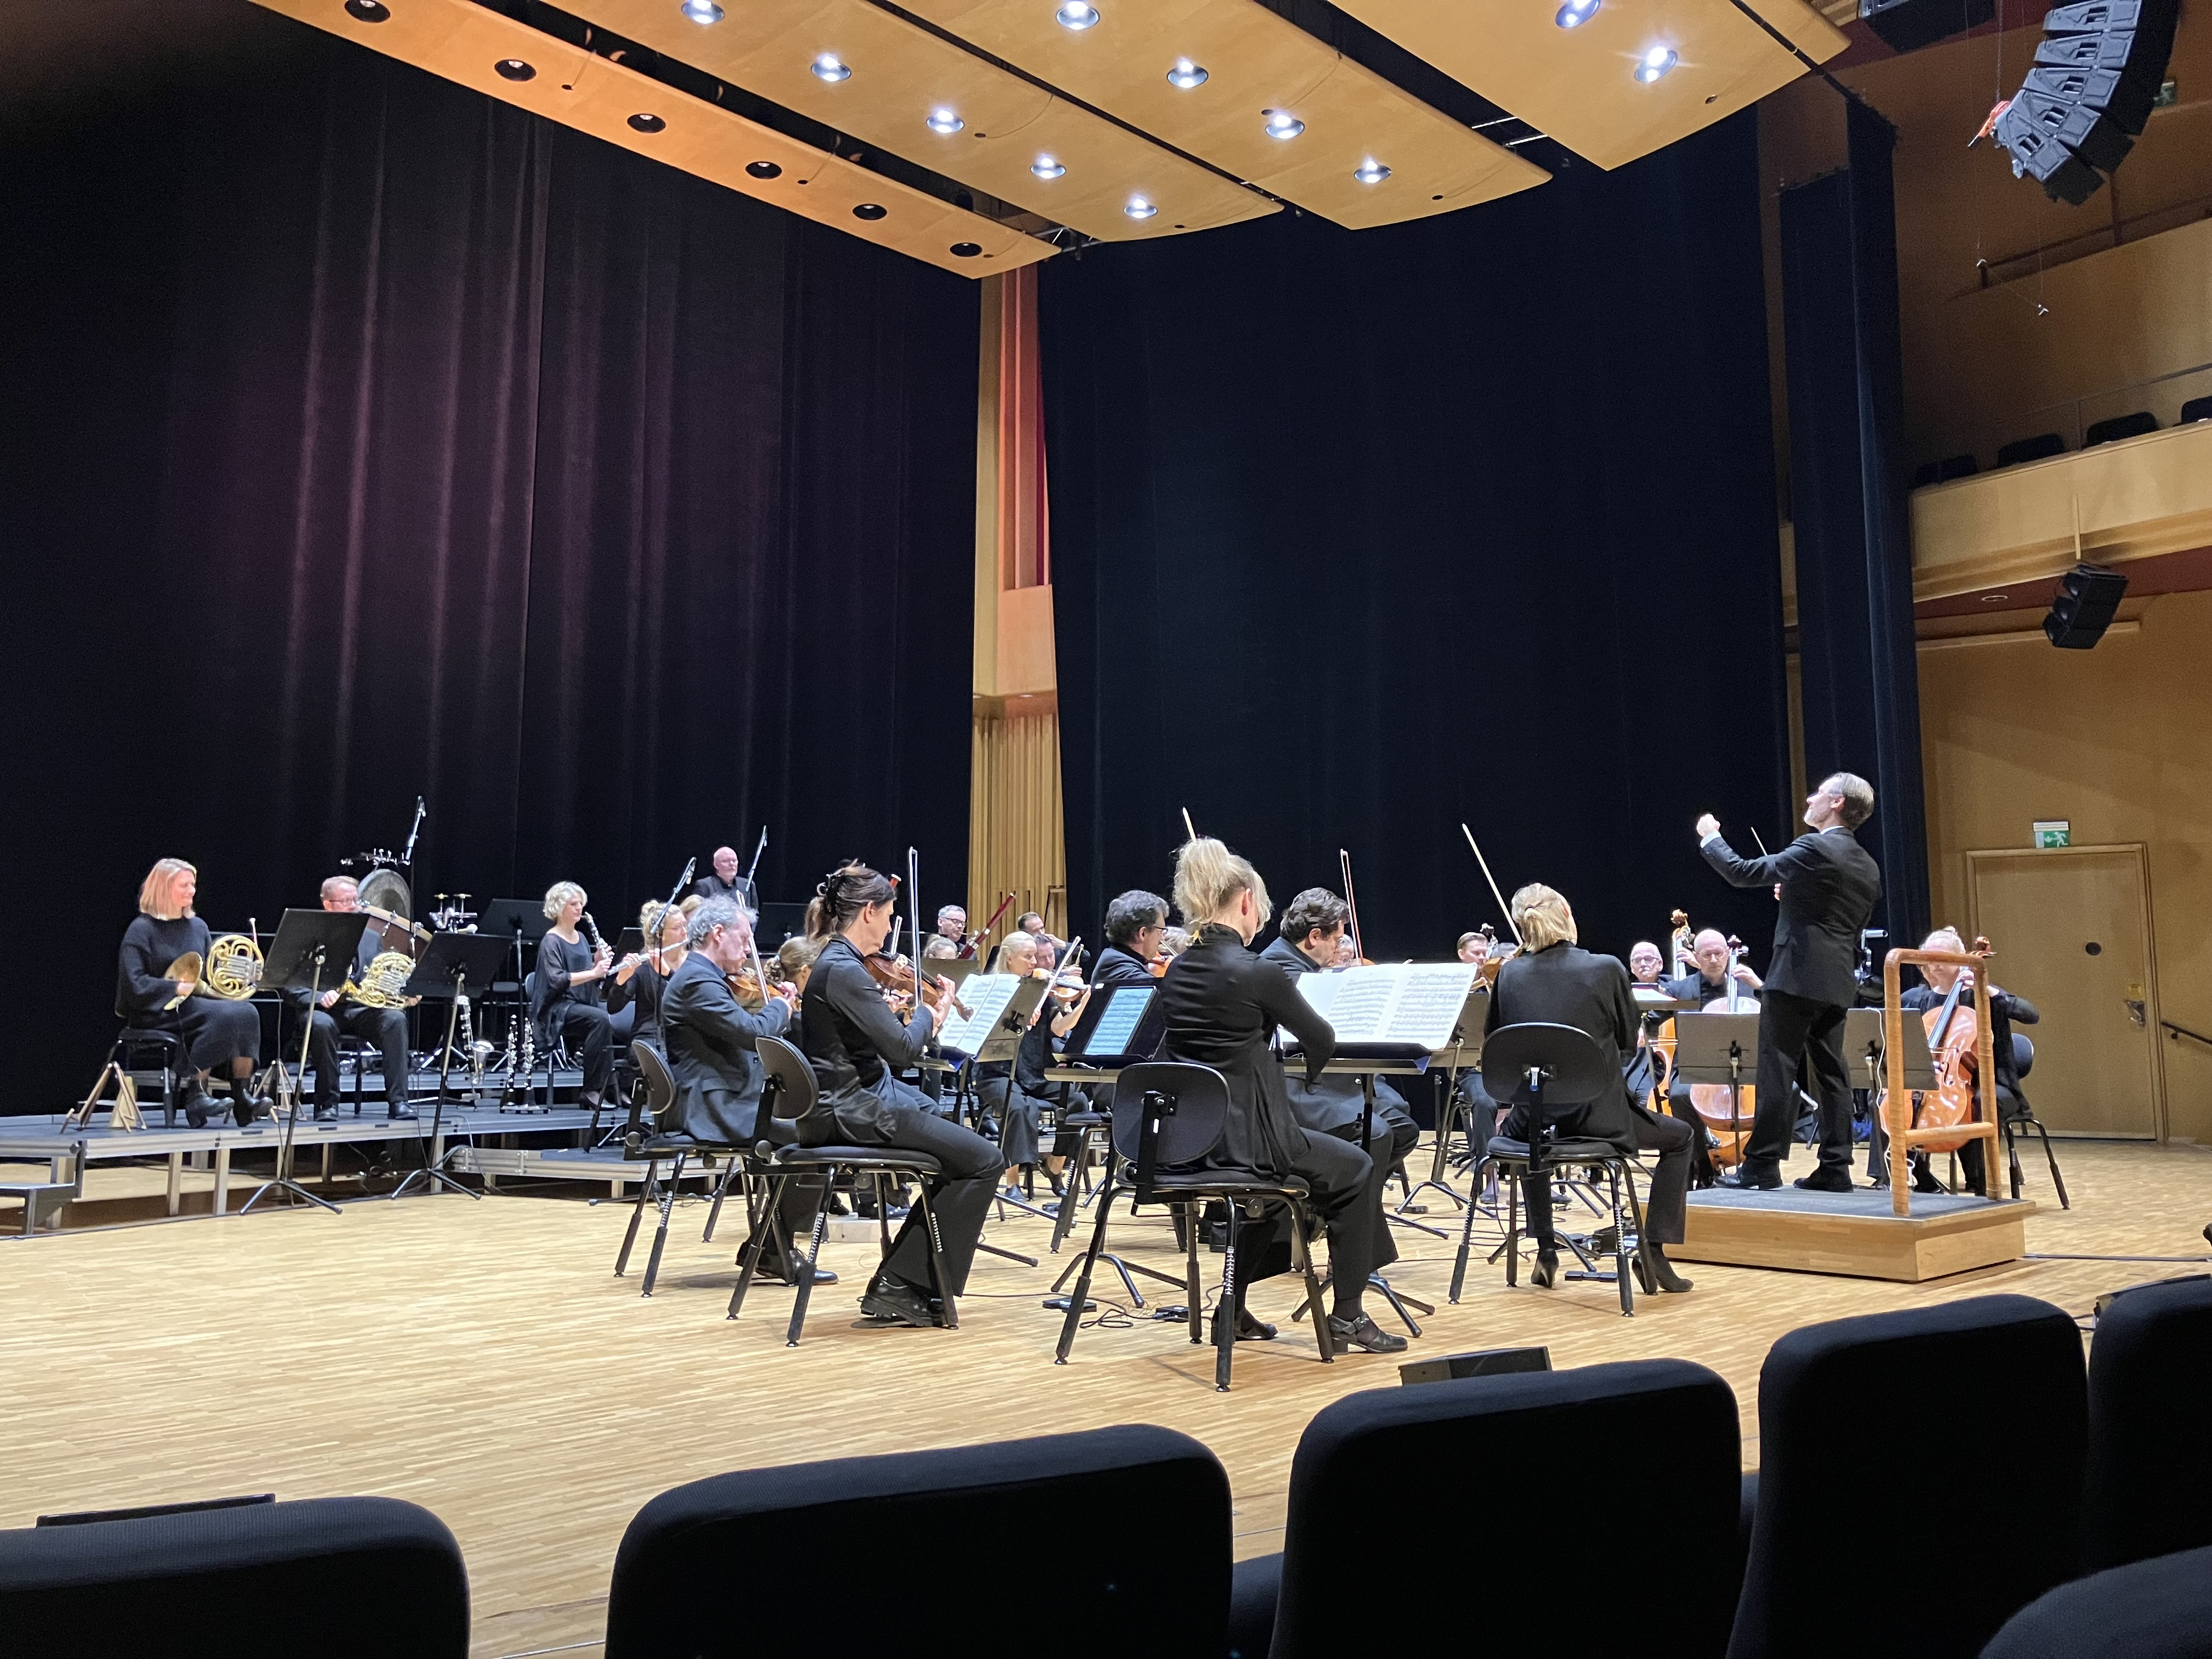
\includegraphics[width=6.5cm, keepaspectratio]{img/IMG_1004.jpg}};
    \end{tikzpicture}
    \caption{Auxtrument concert, Nov. 14 2025, Västerås}
  \end{figure}
\end{frame}

\begin{frame}
  \paperslide
    {Paper I}
    {franklinDevelopmentWebBasedRealTime2025}
    {16cm}
    {../kappa/external_pages/JAES_V73_12_PG872hirez_Franklin.pdf}
    {Technical aspects often overshadow artistic intention.}
\end{frame}

\begin{frame}
  \frametitle{Literature review(s)}
  % \centering
  \moveleft 0.05\textwidth \hbox{
    \resizebox{1.08\textwidth}{!}{
      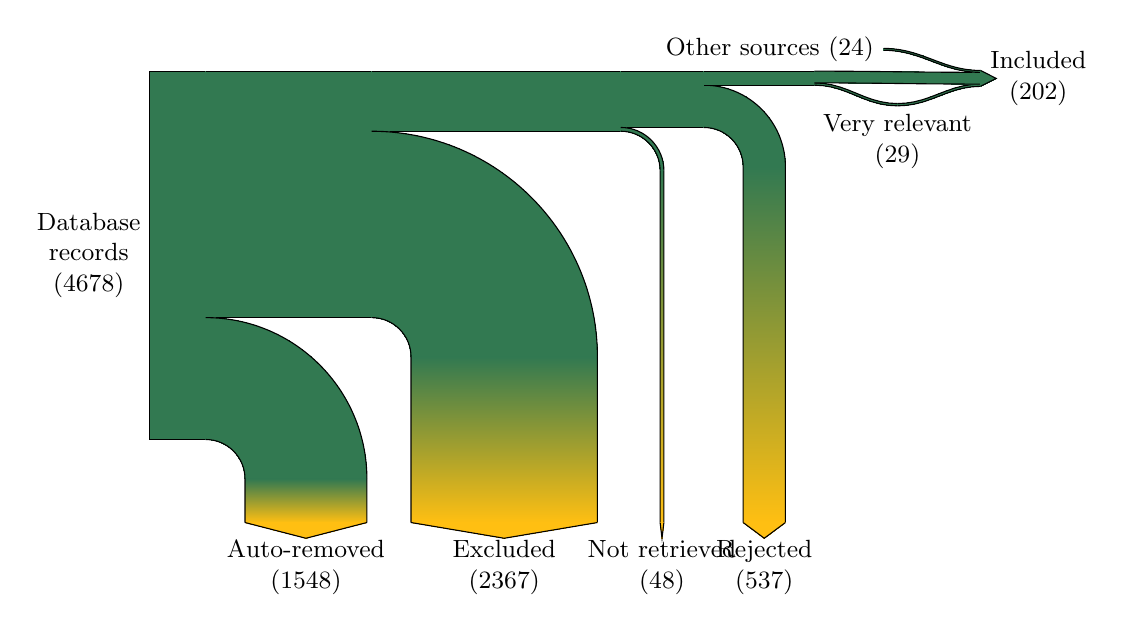
\begin{tikzpicture}[font=\small]
      \begin{sankeydiagram}
    \sankeyset{
        ratio quantity=1000,
        start style=simple, end style=simple,
        records/.style={
            fill/.style={
                line width=0pt,
                draw=MDUsuccess,
                fill=MDUsuccess,
            },
        },
        fade/.style={
            fill/.style={
                fill=none,
                top color=MDUsuccess,
                bottom color=MDUwarning,
                line width=0pt,
            },
        },
        rejected/.style={
            fill/.style={
                fill=MDUwarning,
                draw=MDUwarning,
                line width=0pt,
            },
        },
    }

    \sankeyset{records}
    \sankeynodestart{name=p0,at={0,0},angle=0,quantity=4678}
    \path (p0.right) ++(0,-30pt) coordinate (c);

    \newcommand\turnandstop[2]{ % valname, label
        \begingroup
        \sankeyturnright{#1}{90}
        \sankeynode{as=#1,name=#1-stop,at={#1 |- c}}
        \sankeyset{fade}
        \sankeyoutin{#1}{#1-stop}
        \sankeyset{rejected}
        \sankeynode{as=#1-stop,name=#1}
        \sankeyend{#1}
        \node[below, align=center] at ([yshift=-3pt]#1) {#2\\(\sankeygetnodeqty{#1})};
        \endgroup
    }

    \node[left,align=center] at (p0) {Database\\records\\(4678)};
    \sankeyadvance{p0}{20pt};
    
    \sankeyfork{p0}{3130/p1,1548/p2}
    \sankeyadvance{p1}{60pt}
    \turnandstop{p2}{Auto-removed}
    
    \sankeyfork{p1}{763/p4,2367/p5}
    \sankeyadvance{p4}{90pt}
    \turnandstop{p5}{Excluded}

    \sankeyfork{p4}{715/p6,48/p7}
    \sankeyadvance{p6}{30pt}
    \turnandstop{p7}{Not retrieved}

    \sankeyfork{p6}{178/p8,537/p9}
    \turnandstop{p9}{Rejected}
    \sankeyadvance{p8}{40pt}

    \sankeyfork{p8}{149/p10,29/p11};
    \sankeynode{
        name=veryrelevant,
        at={[shift={(30pt,-10pt)}]p10},
        quantity=29
    };
    \node[below, align=center] at (veryrelevant) {Very relevant\\(29)};

    \sankeynode{
        name=included,
        at={[xshift=60pt,yshift=-0.5pt]p10},
        quantity=202, 
        forked={24/p20,149/p21,29/p22}
    };
    
    \sankeynodestart{name=p12,at={[xshift=25pt, yshift=10pt]p10},angle=0,quantity=24}
    \node[left,align=center] at (p12) {Other sources (24)};

    \sankeyoutin{p11}{veryrelevant}
    \sankeyoutin{veryrelevant}{p22}
    \sankeyoutin{p10}{p21}
    \sankeyoutin{p12}{p20}
    \sankeyend{included}
    \node[right,align=center] at (included) {Included\\(202)};

\end{sankeydiagram}
      \end{tikzpicture}
    }
  }
\end{frame}

\begin{frame}
  \paperslide
    {Paper II}
    {miticSystematicLiteratureReview2026}
    {16cm}
    {../kappa/external_pages/s13636-026-00463-4.pdf}
    {Techniques for describing stereo image exist, but their effectiveness is understudied.}
\end{frame}

\begin{frame}
  \frametitle{Software(s)}
  \centering
  \def\plotheight{7cm}
  \def\plotheightthin{3cm}
  \begin{tikzpicture}[inner sep=0pt]
    \node[anchor=north west] (code) at (0,0) {
      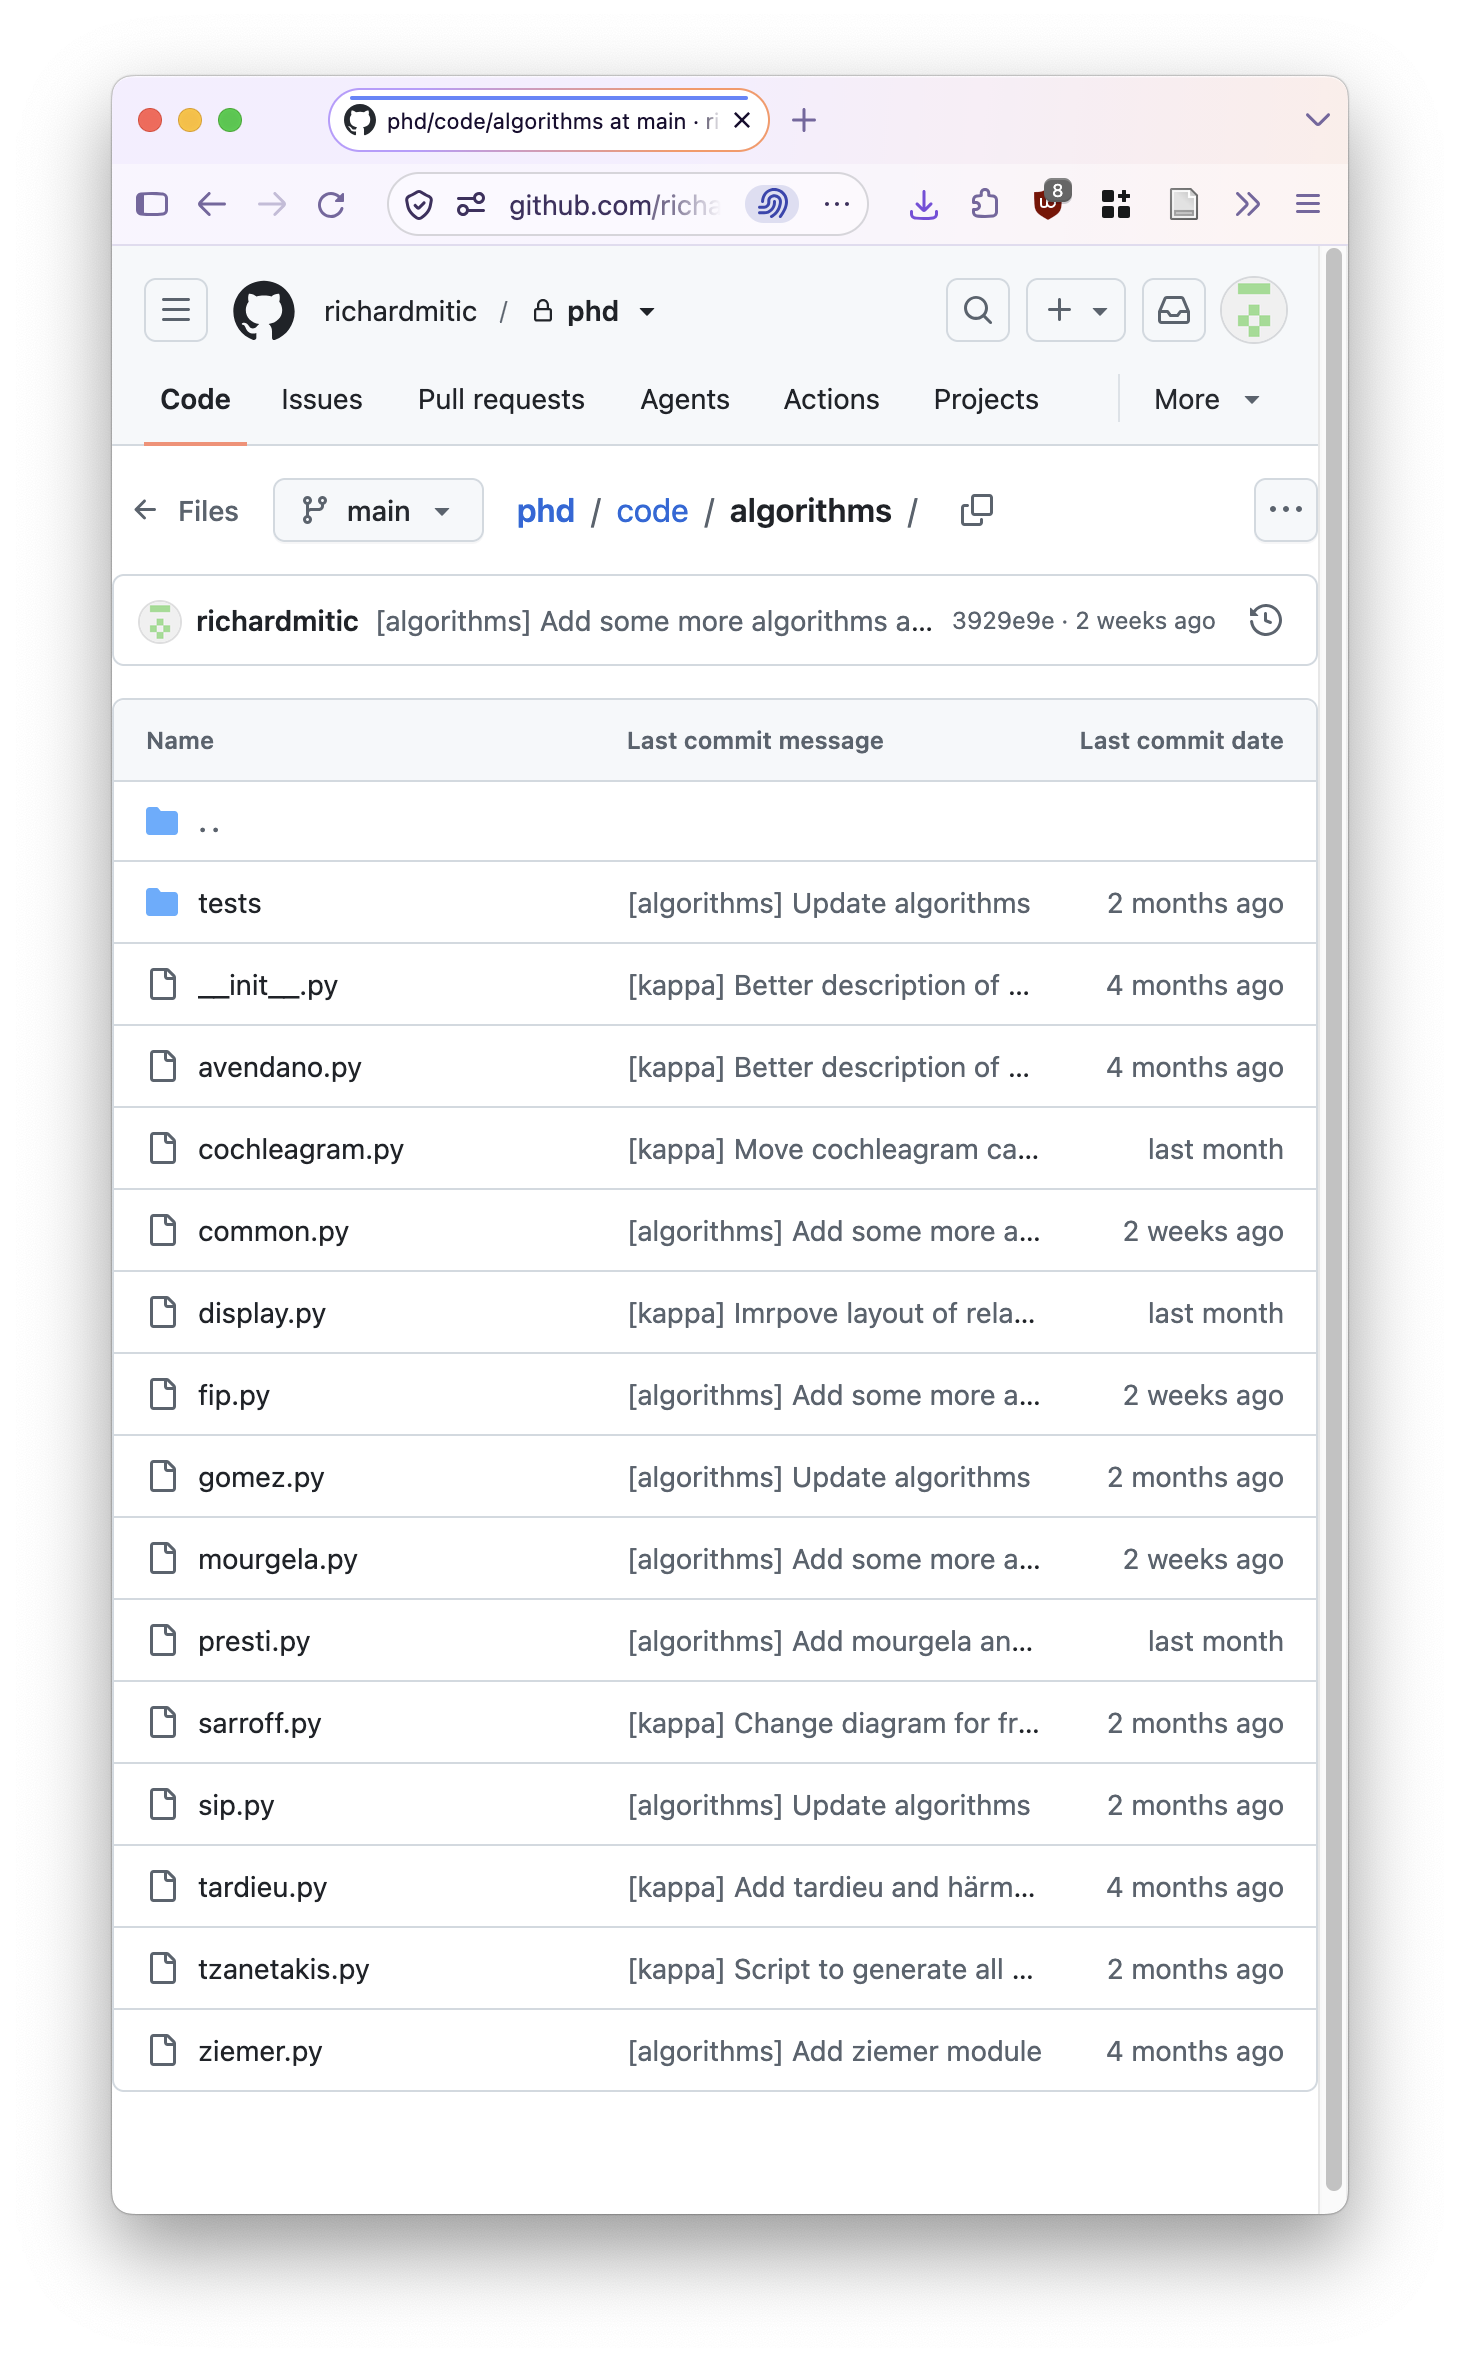
\includegraphics[height=\plotheight, keepaspectratio]{code.png}\footnote{\url{https://github.com/richardmitic/phd}}
    };
    \node[anchor=north east, outer sep=0.3cm] (spf) at (12,0) { 
      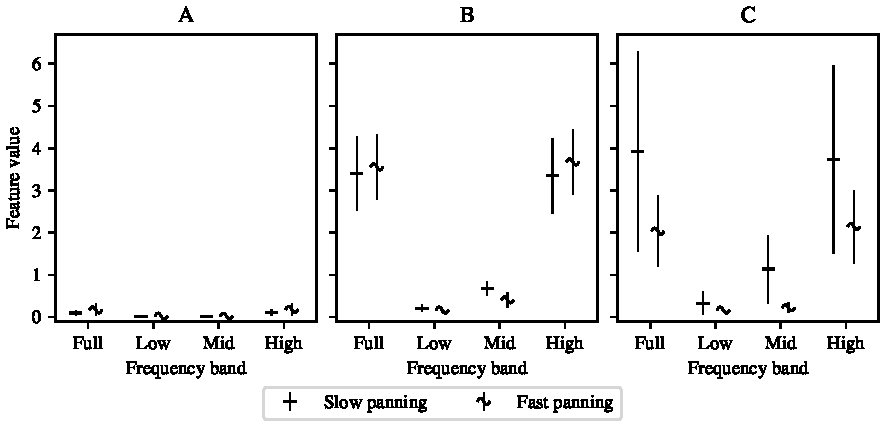
\includegraphics[height=\plotheightthin, keepaspectratio]{spf.pdf}
    };
    \node[anchor=south east, outer sep=0.3cm] (ph) at (code.south -| spf.east) { 
      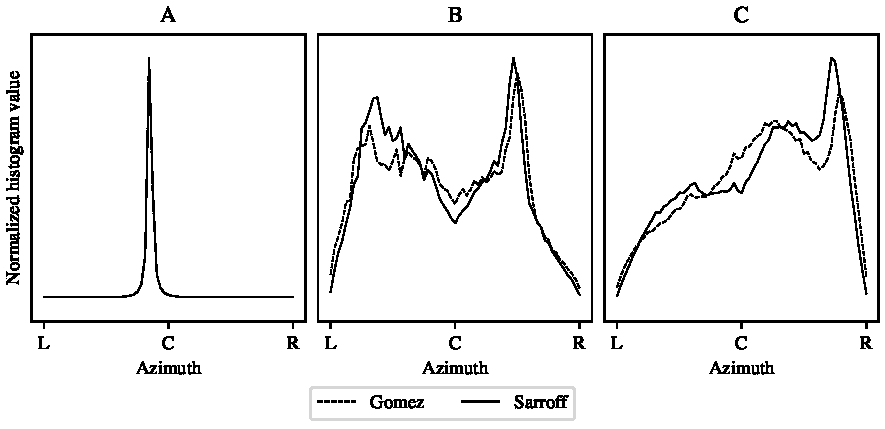
\includegraphics[height=\plotheightthin, keepaspectratio]{panning_histograms.pdf}
    };
  \end{tikzpicture}
\end{frame}

\begin{frame}
  \frametitle{Panning histograms\footcite{sarroffMeasurementsSpaciousnessStereophonic2008,gomezMusicSimilaritySystems2008}}
  \centering
  \begin{tikzpicture}[every node/.style={scale=0.9}]
    \node {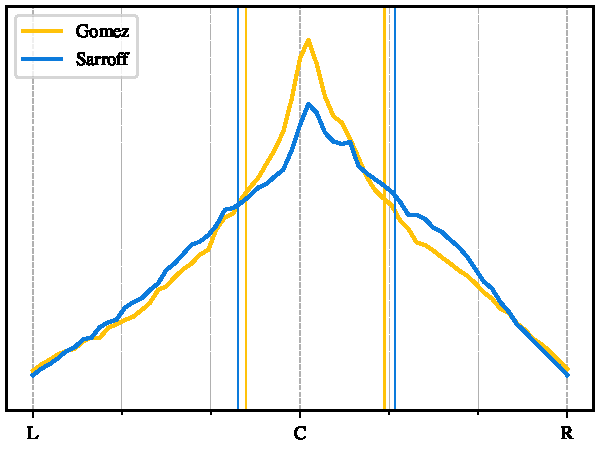
\includegraphics[angle=0]{generated/ph_2.pdf}};
    \pause
    \node {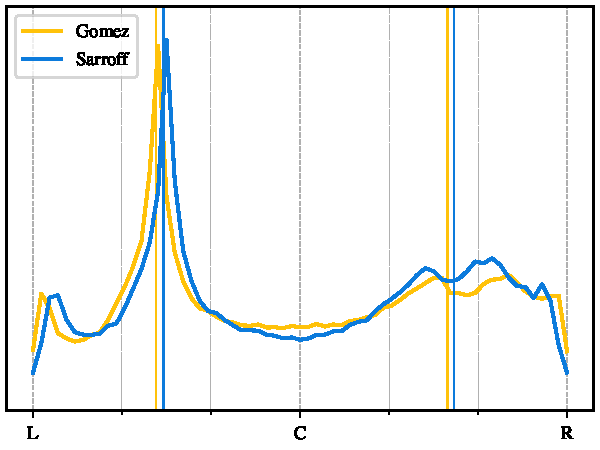
\includegraphics[angle=5]{generated/ph_1.pdf}};
    \pause
    \node {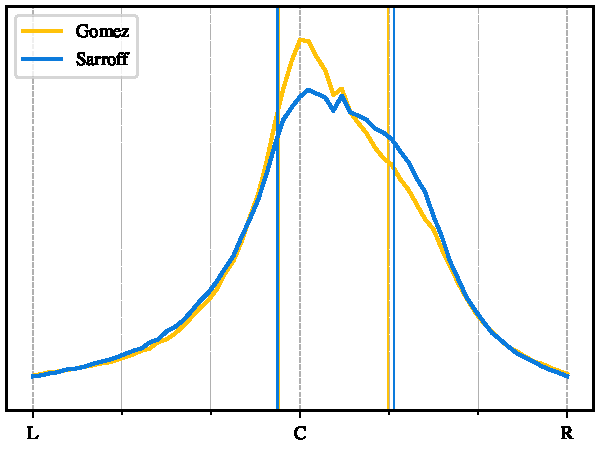
\includegraphics[angle=-2]{generated/ph_3.pdf}};
    \pause
    \node {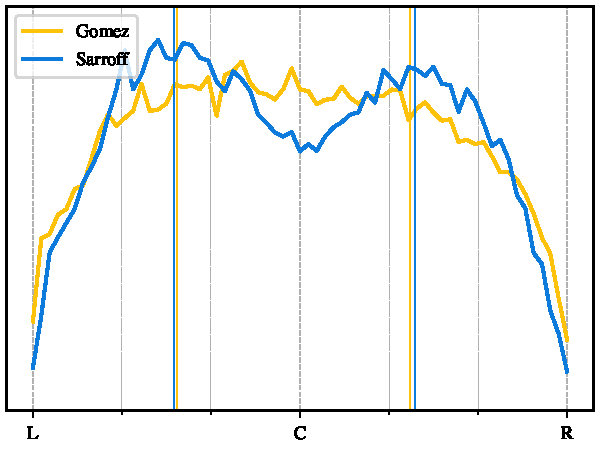
\includegraphics[angle=4]{generated/ph_4.pdf}};
    \pause
    \node {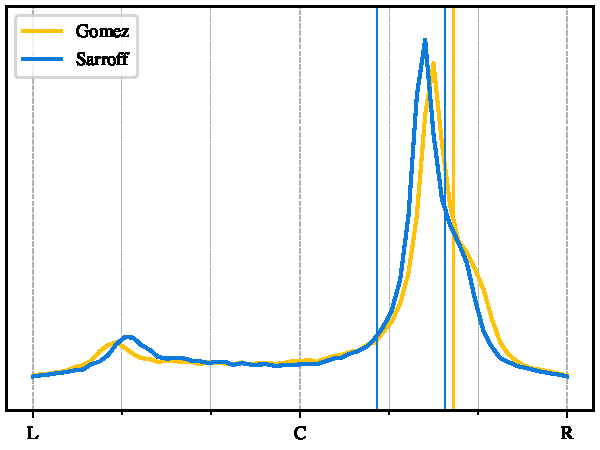
\includegraphics[angle=1]{generated/ph_5.pdf}};
    \pause
    \node {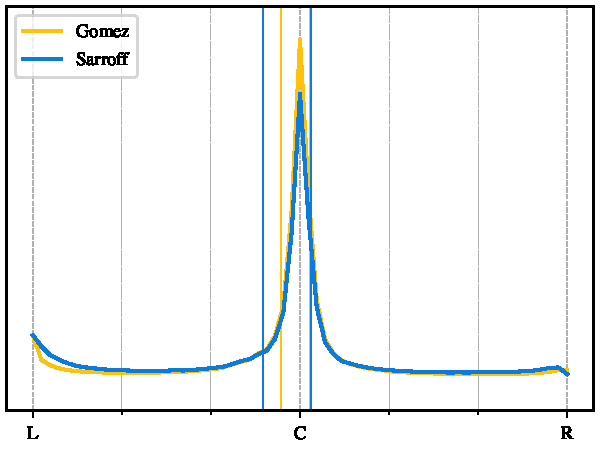
\includegraphics[angle=-3]{generated/ph_6.pdf}};
  \end{tikzpicture}
\end{frame}

\begin{frame}
  \frametitle{Panning histograms\footcite{sarroffMeasurementsSpaciousnessStereophonic2008,gomezMusicSimilaritySystems2008}}
  \centering
  \only<1>{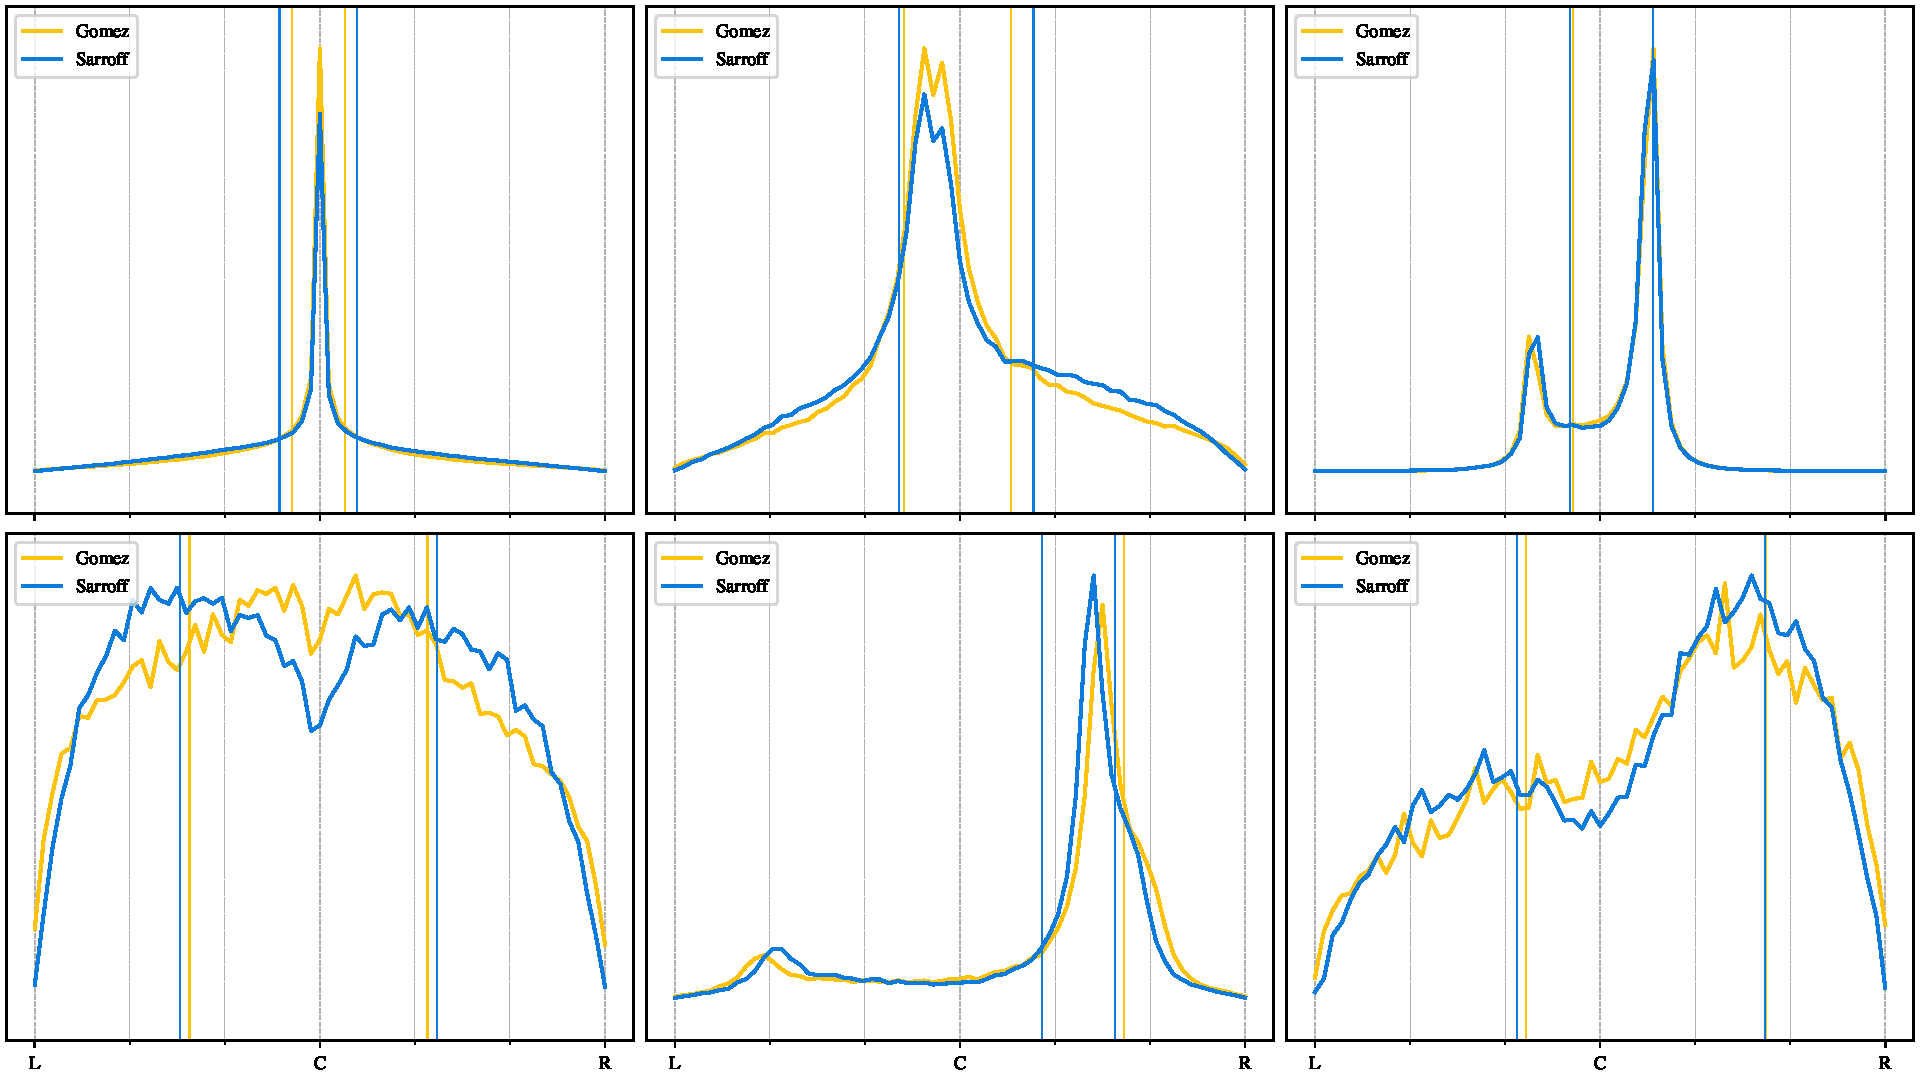
\includegraphics[height=0.8\textheight]{generated/grids/ph_grid_3x2.pdf}}
  \only<2>{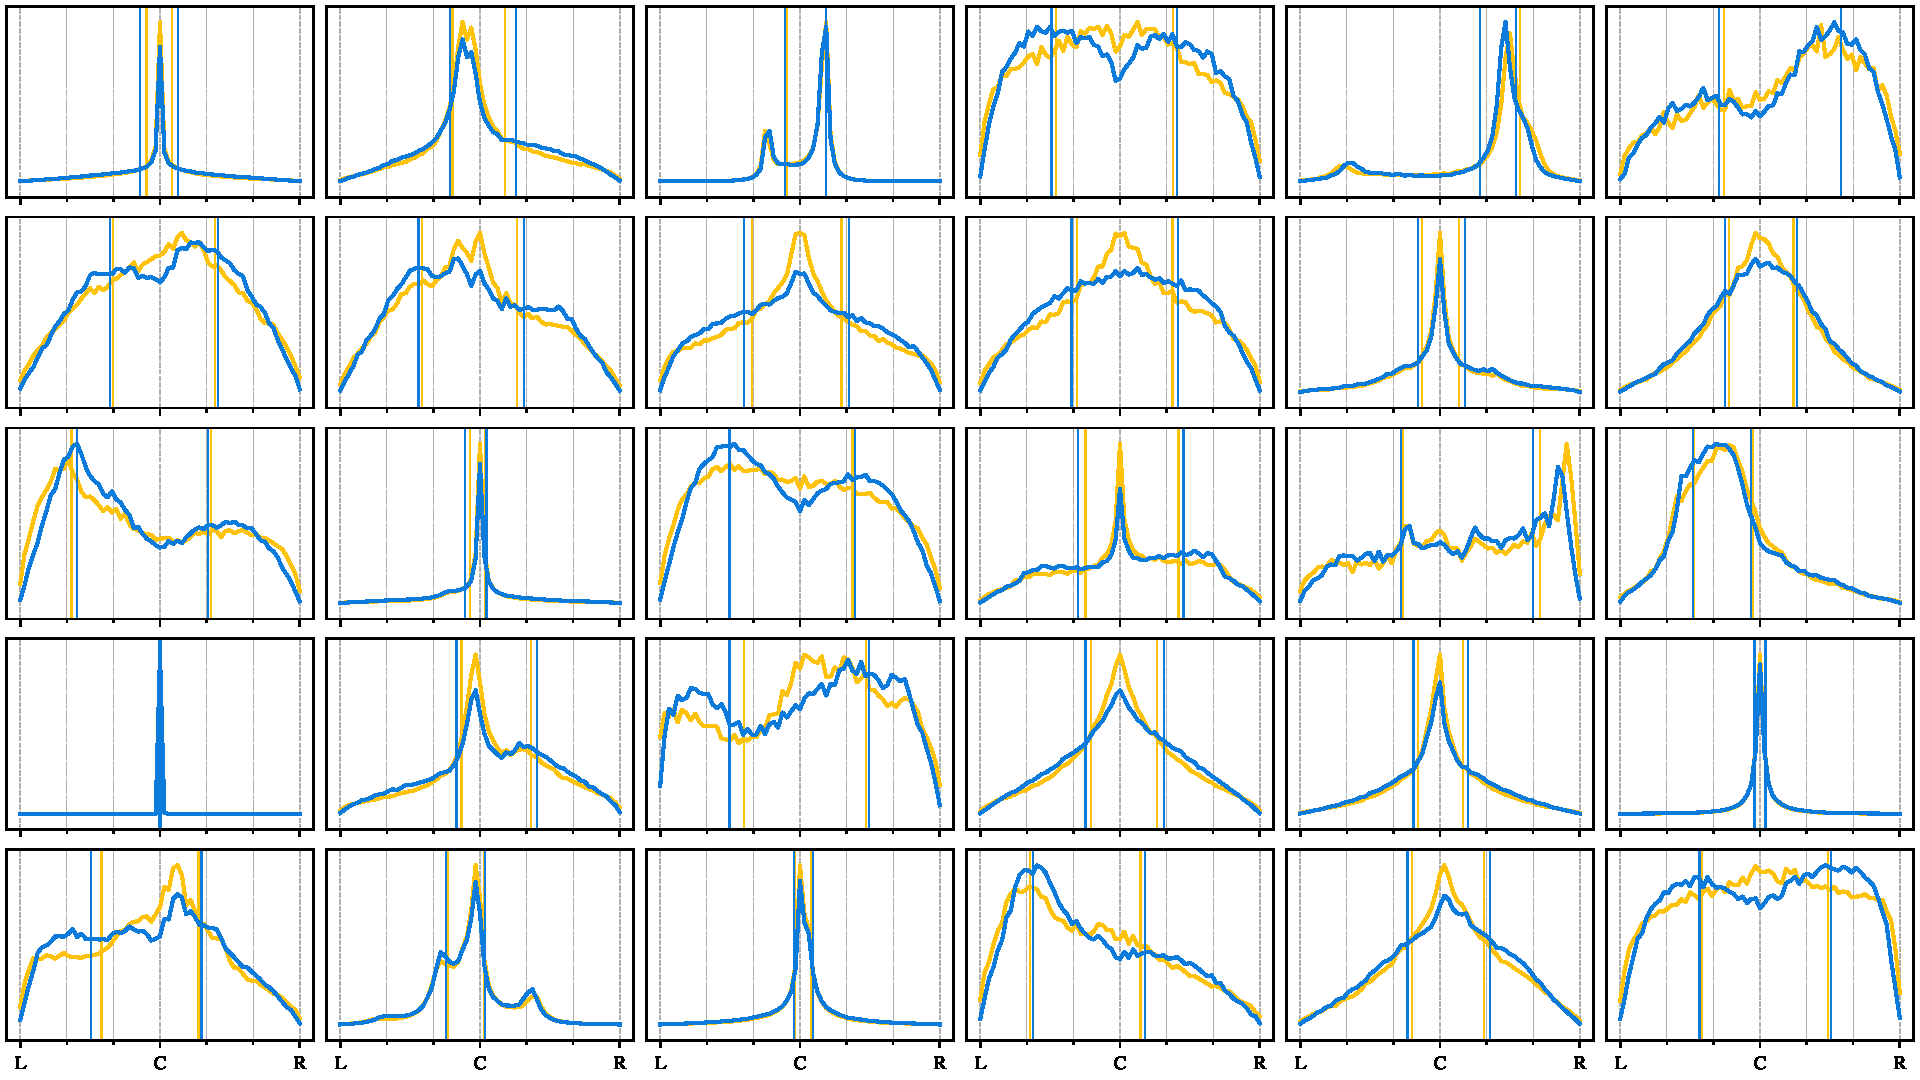
\includegraphics[height=0.8\textheight]{generated/grids/ph_grid_6x5.pdf}}
  \only<3>{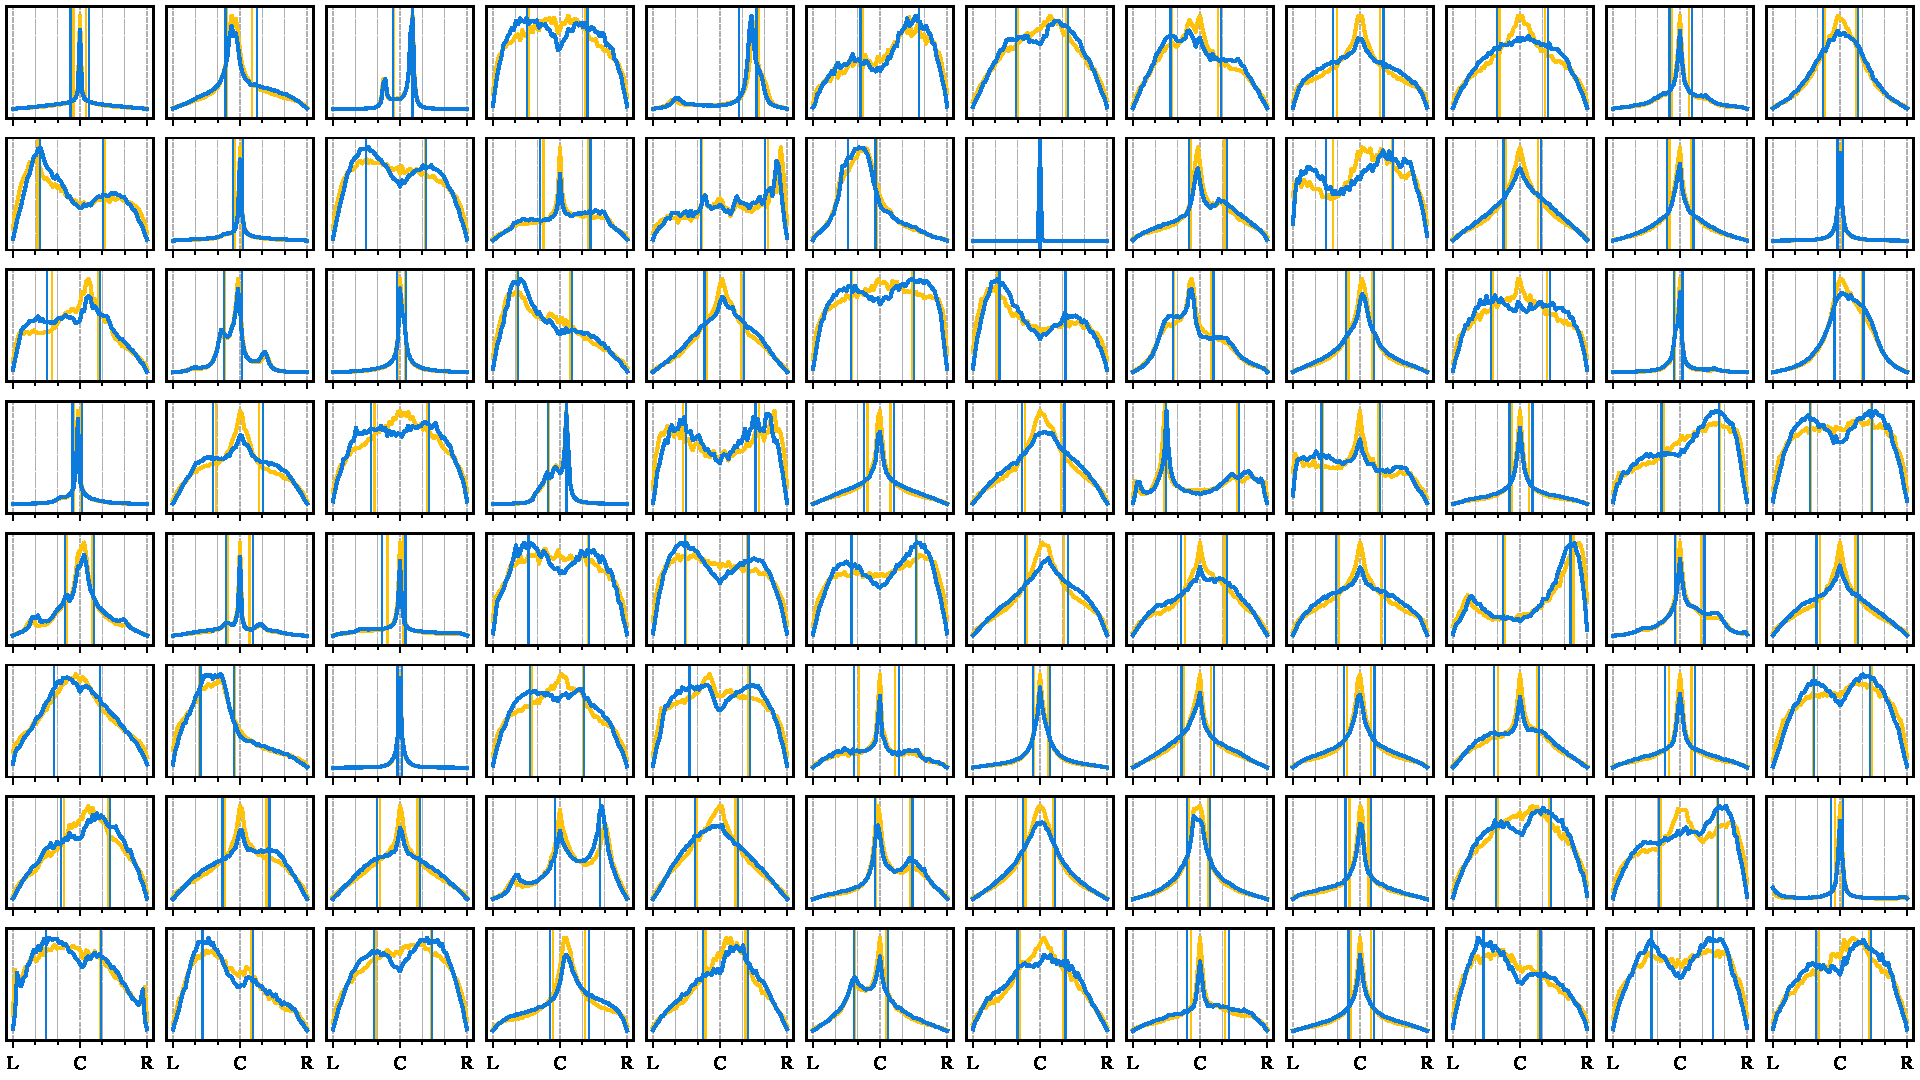
\includegraphics[height=0.8\textheight]{generated/grids/ph_grid_12x8.pdf}}
\end{frame}

\begin{frame}
  \frametitle{Goniometers\footcite{ziemerGoniometersArePowerful2023}}
  \centering
  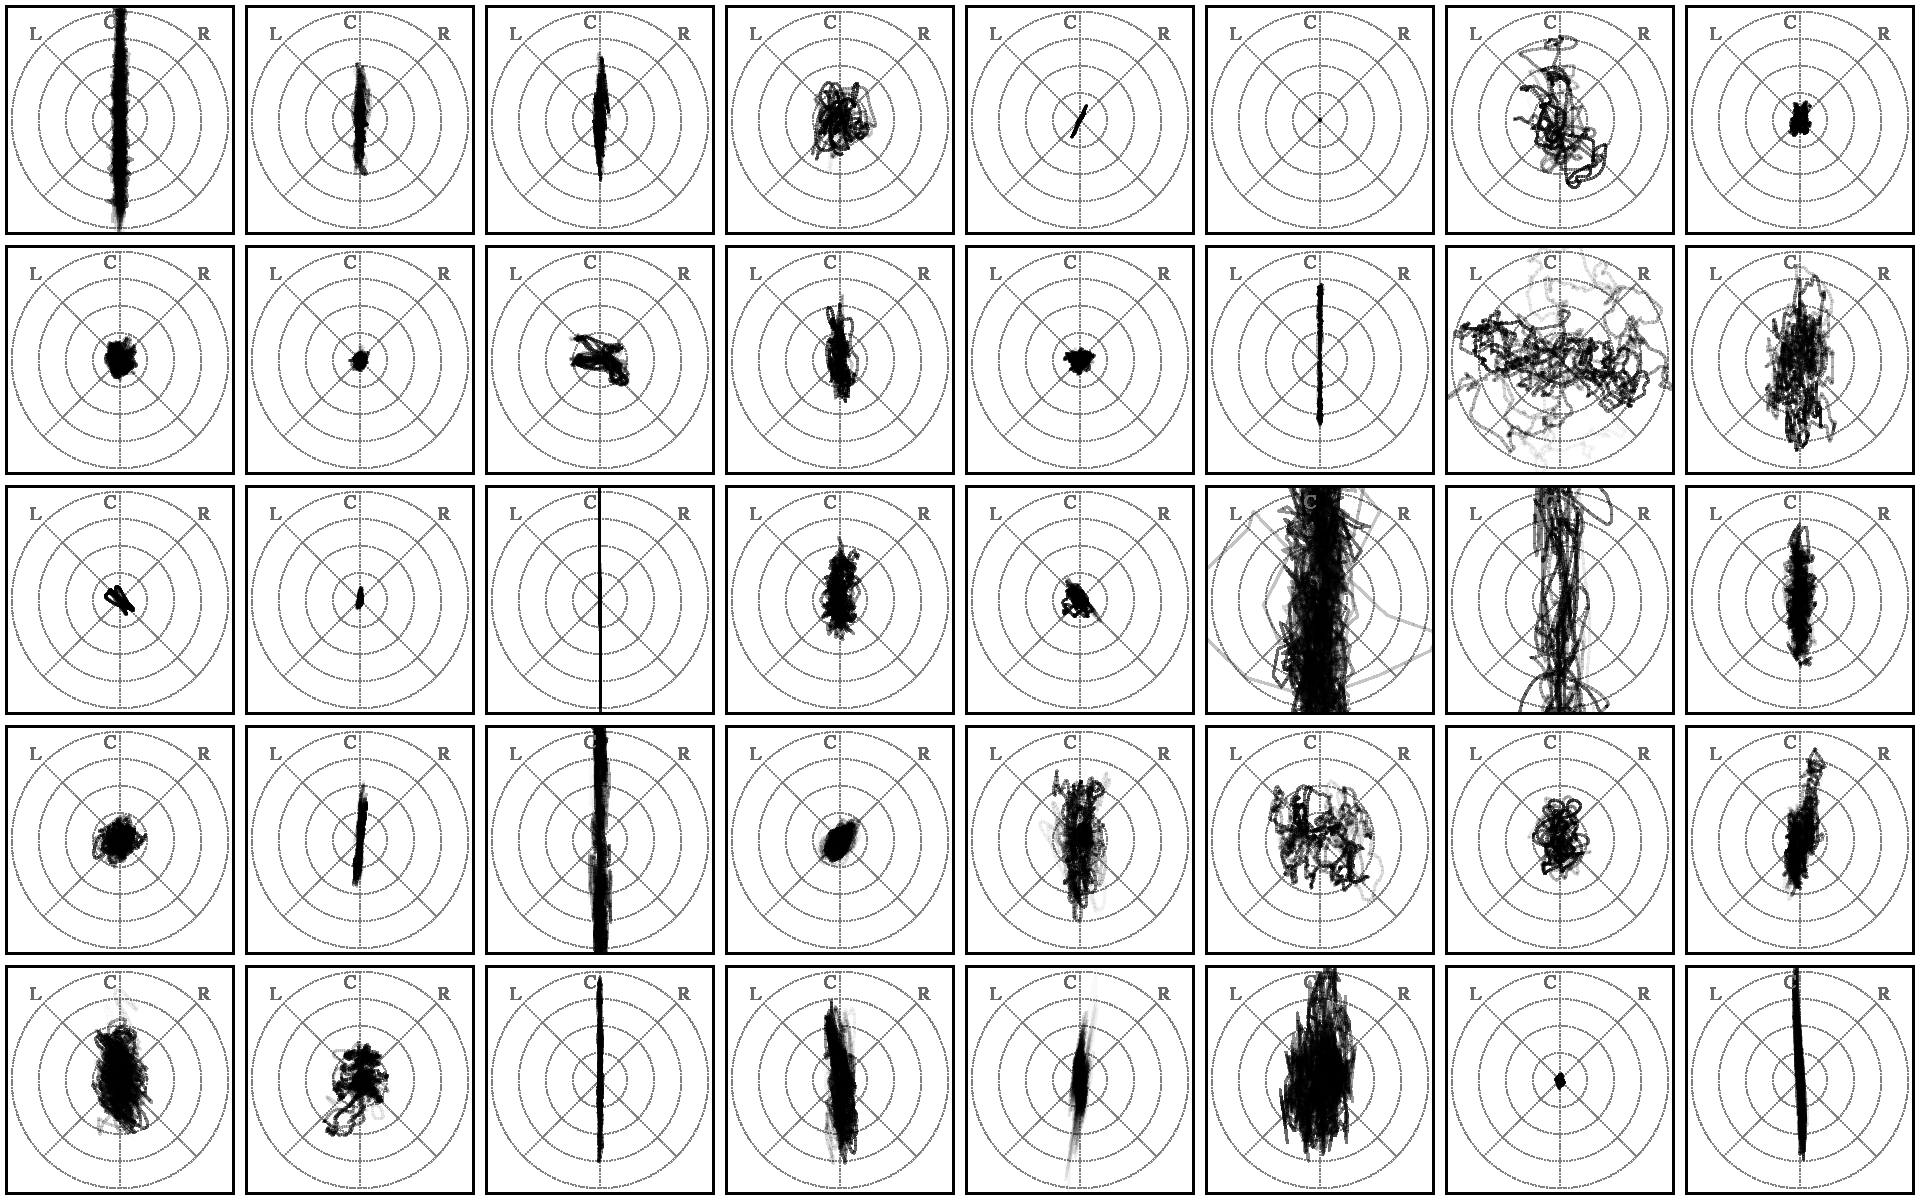
\includegraphics[height=0.8\textheight]{generated/grids/gonio_grid_8x5.pdf}
\end{frame}

\begin{frame}
  \frametitle{Stereo Panning Features\footcite{tzanetakisStereoPanningFeatures2007}}
  \centering
  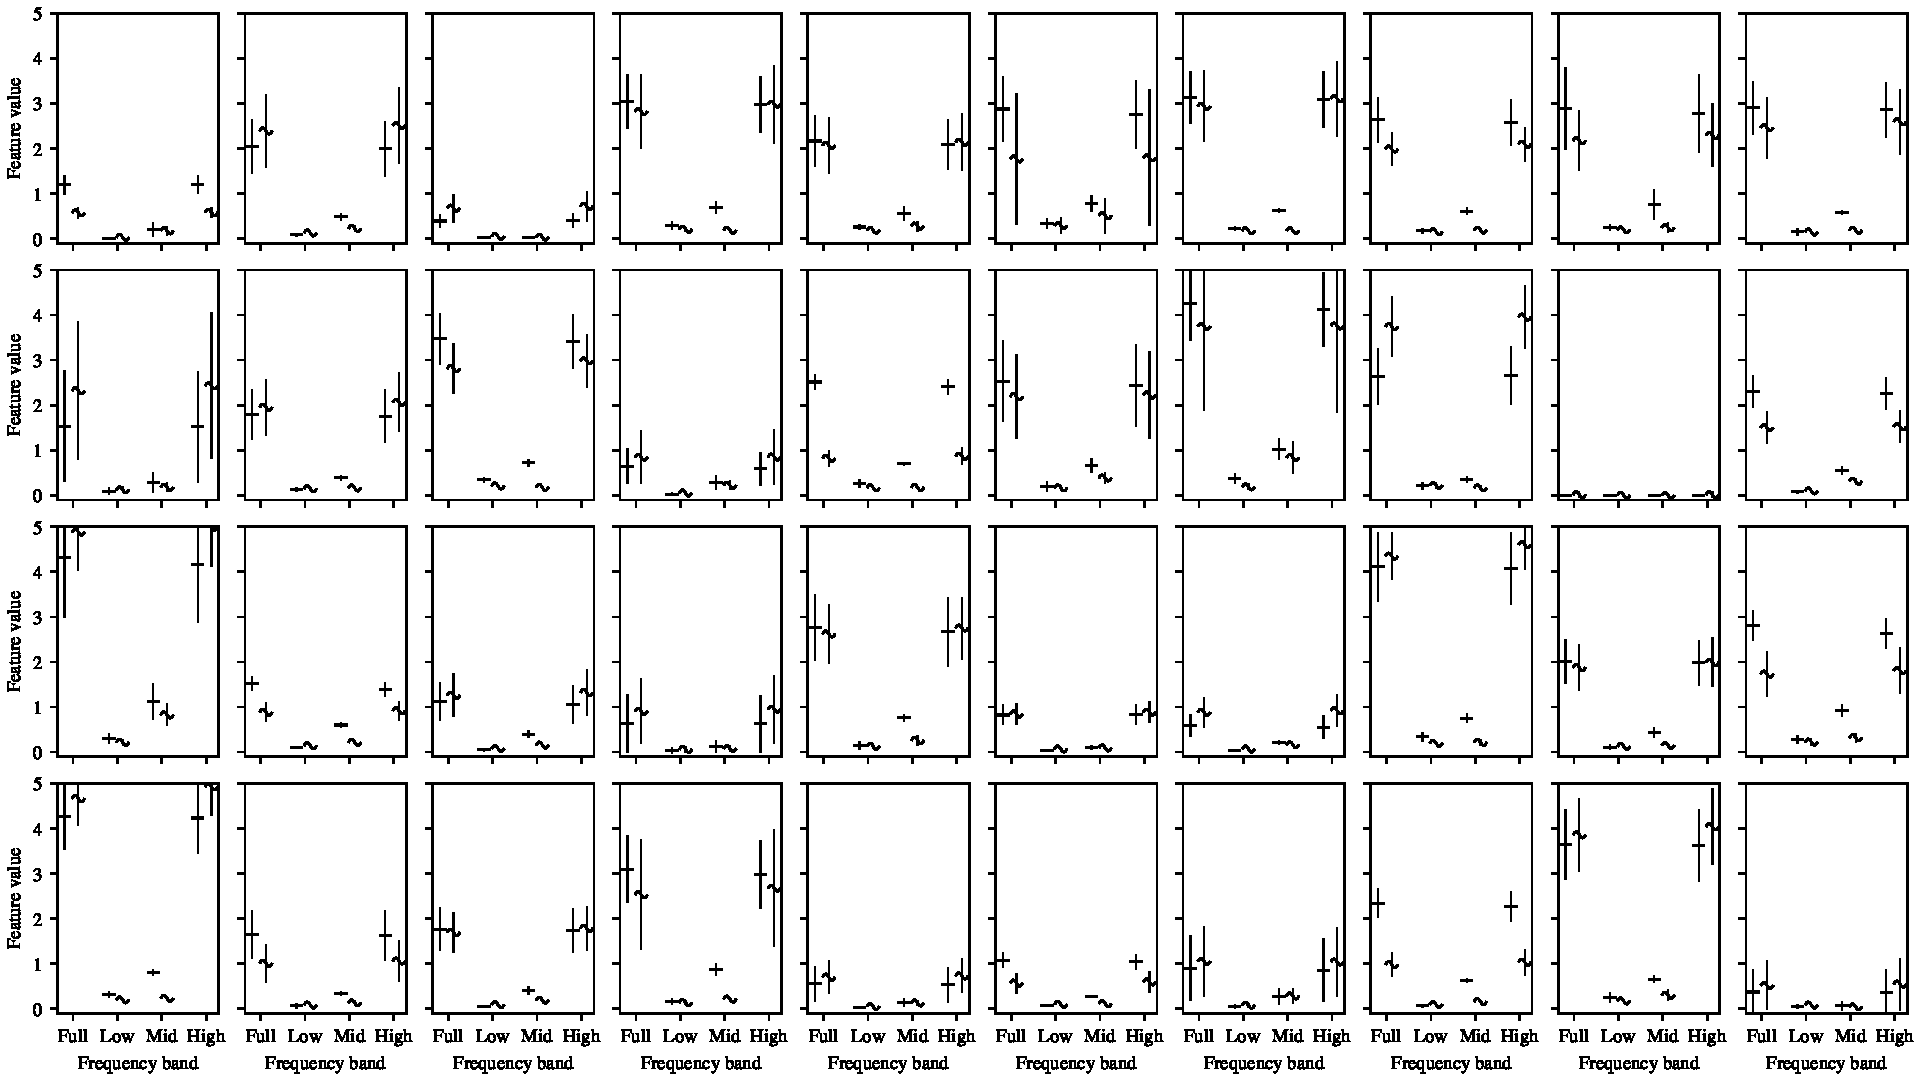
\includegraphics[height=0.8\textheight]{generated/grids/spf_grid_10x4.pdf}
\end{frame}

\begin{frame}
  \frametitle{Amplitude Panning Features\footcite{tardieuProductionEffectAudio2011}}
  \centering
  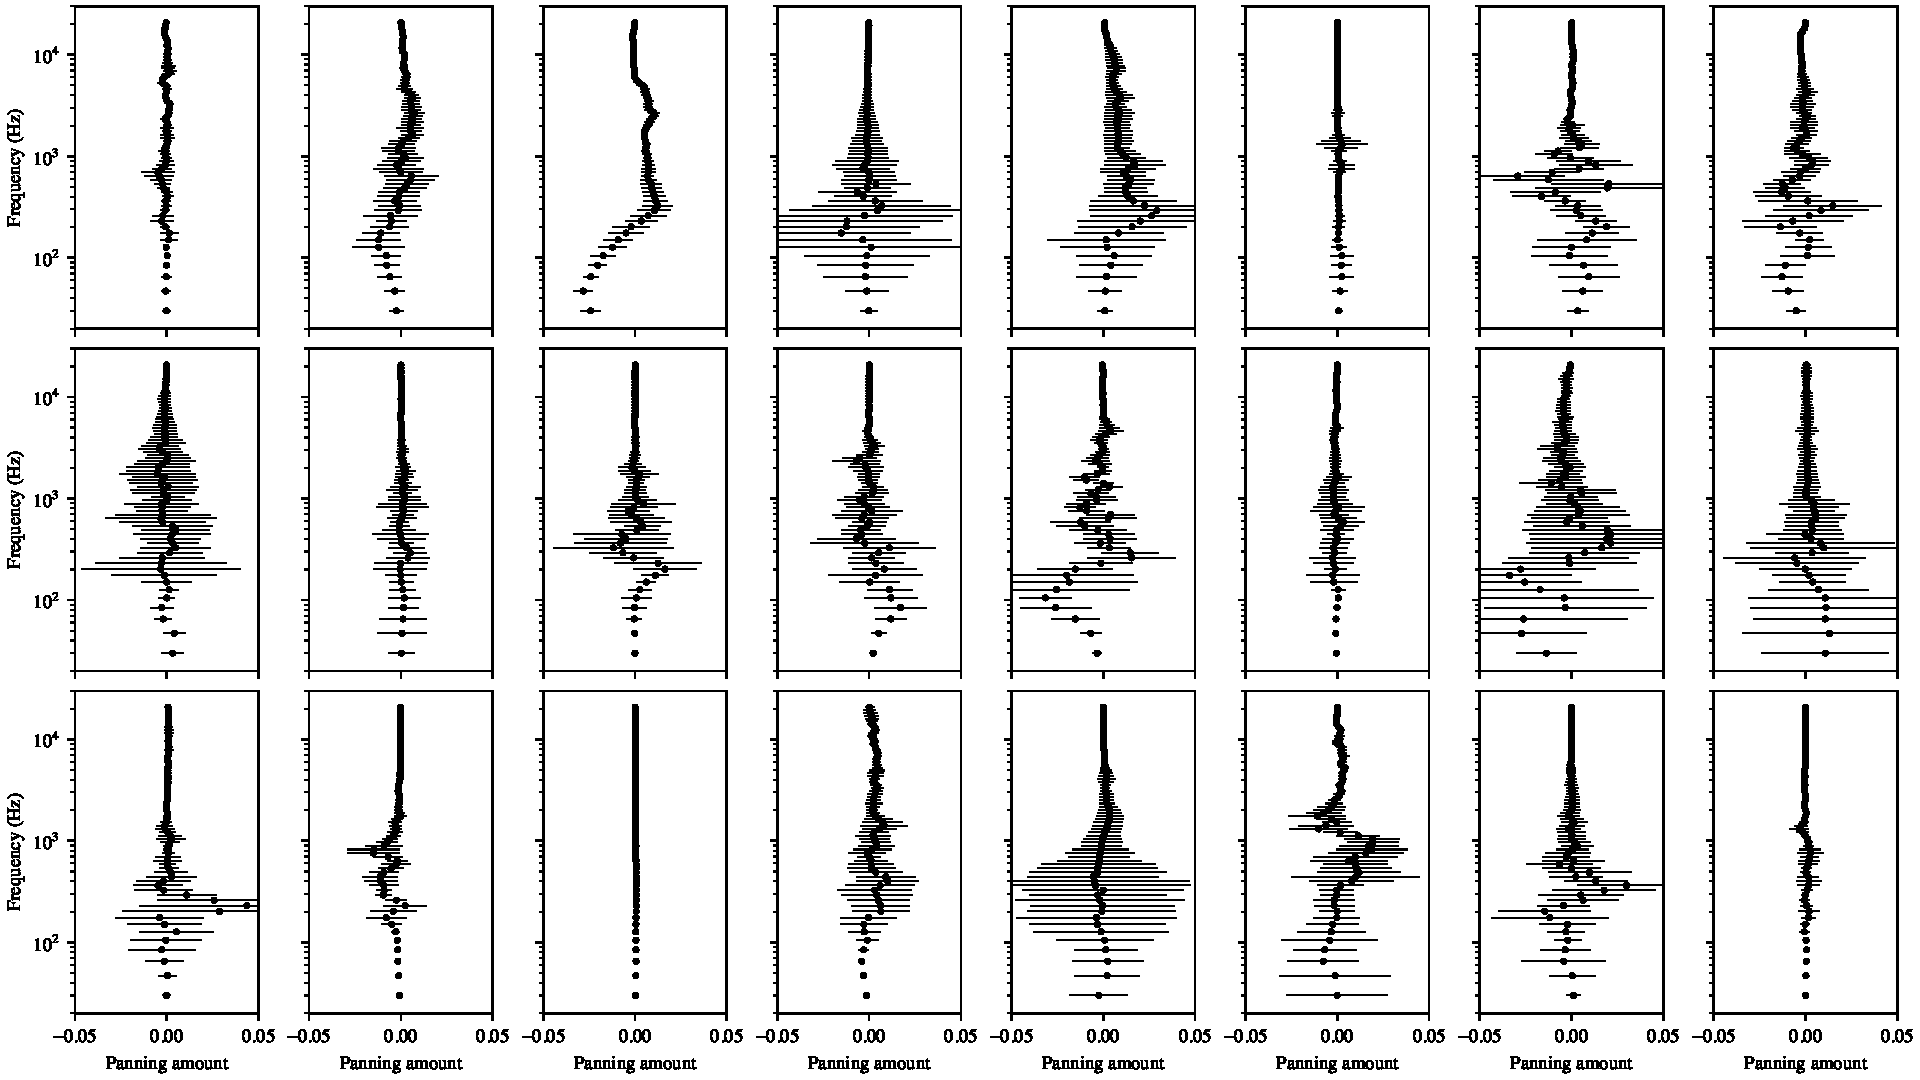
\includegraphics[height=0.8\textheight]{generated/grids/asf_grid_8x3.pdf}
\end{frame}

\begin{frame}
  \frametitle{Finding similar stereo fields}
  \centering
  \only<1>{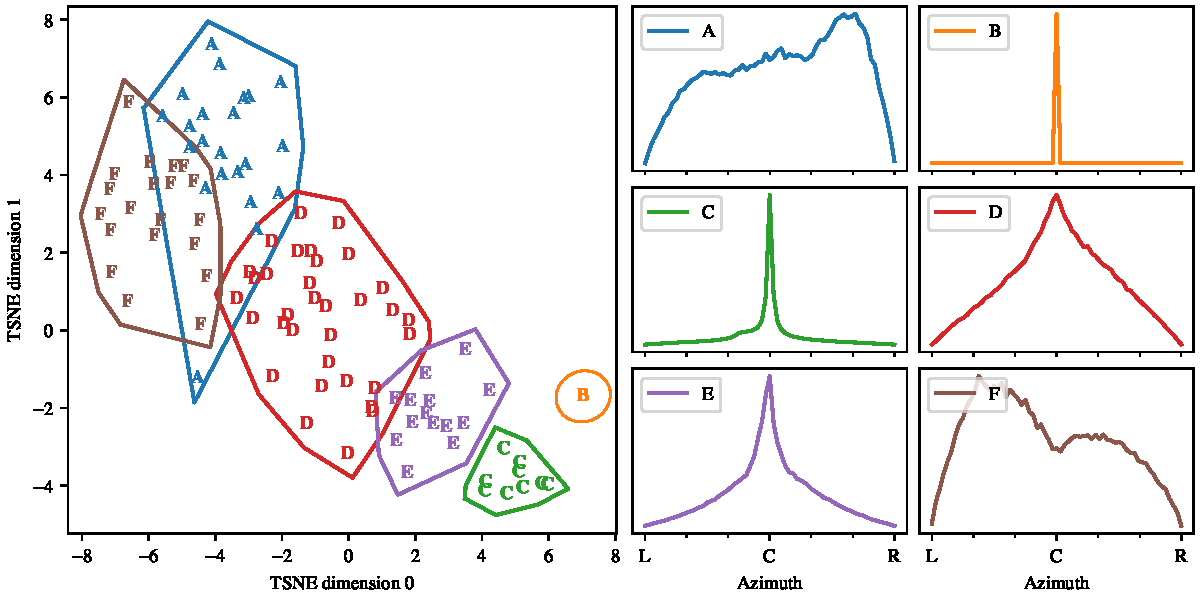
\includegraphics[width=\textwidth]{generated/clusters.pdf}}
  \only<2>{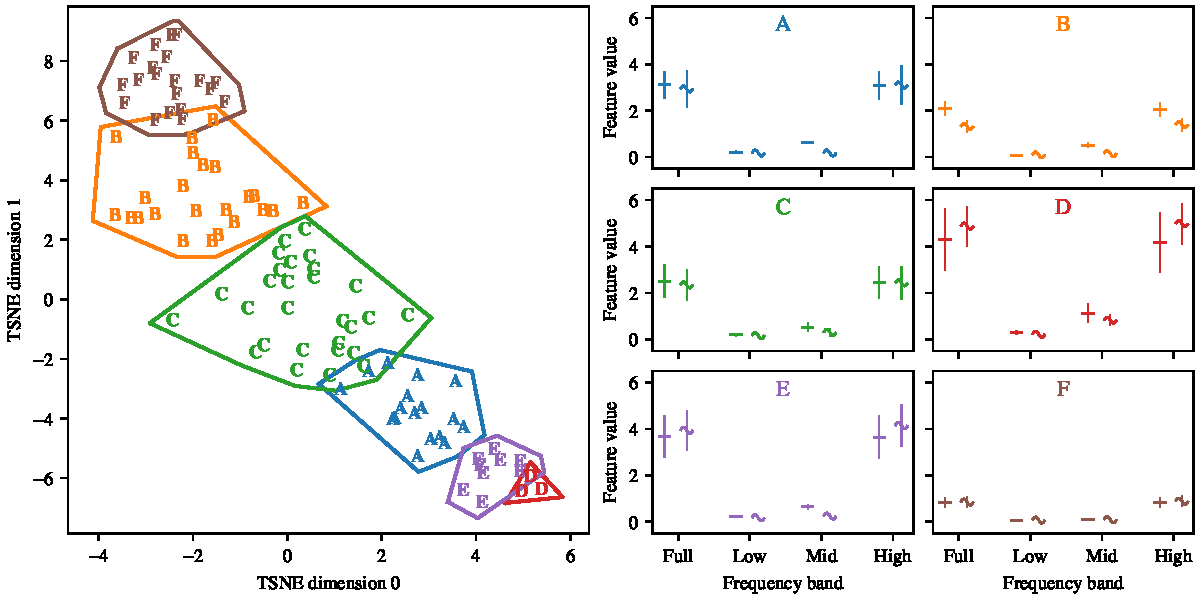
\includegraphics[width=\textwidth]{generated/clusters_spf.pdf}}
\end{frame}

\begin{frame}
  \paperslide
    {Paper III}
    {miticObjectiveComparisonPanning2025}
    {19cm}
    {../kappa/external_pages/Mitic and Rossholm - 2025 - Towards an objective comparison of panning feature algorithms for unsupervised learning.pdf}
    {All panning feature algorithms have inherent limitations, but Stereo Panning Features offers the most promising results for unsupervised learning.}
\end{frame}

\begin{frame}
  \frametitle{DAFx2025 poster}
  \centering
  \begin{tikzpicture}[
    spy using outlines={
      rectangle,
      magnification=2.5,
      size=6cm,
      connect spies}]
    \node[inner sep=0pt] (img) {\pgfimage[height=0.8\textheight]{../dafx2025_sip_comparison/poster.pdf}};
    \spy[MDUorange] on ([xshift=-1.5]img.center) in node at (.5\textwidth,0);
  \end{tikzpicture}
  \note{We used several tracks that we found from the previous exploration to demonstrate what each panning feature algorithm can "hear". We considered all tracks to make different uses of stereo image, so we judged how well each algorithm was able to differentiate between them.}
\end{frame}

\begin{frame}
  \frametitle{Potential application}
  Mix speech and music using \q{smart} panning

  \begin{center}
    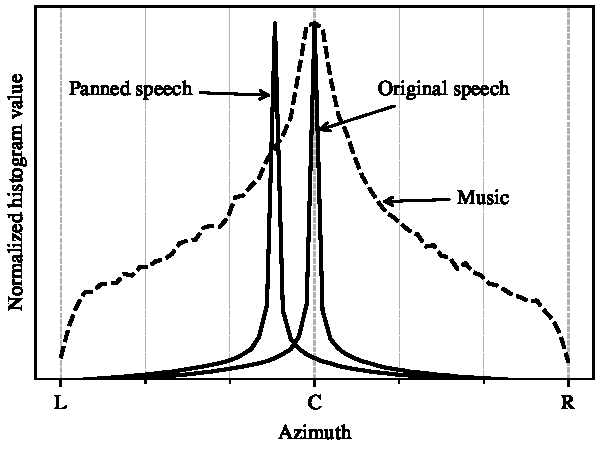
\includegraphics[height=0.7\textheight]{generated/panned_speech.pdf}
  \end{center}
  
  \note{Needed a perceptual test to determine the efficacy.\\}
  \note{Assumptions:\\}
  \note{Music is the primary source \& speech is secondary.\\}
  \note{Panning the speech away from the musical energy will increase pleasantness.\\}
\end{frame}

\begin{frame}
  \frametitle{Perceptual test}
  \centering
  \only<1> {
    \begin{tikzpicture}
      \node at (0,0) {
        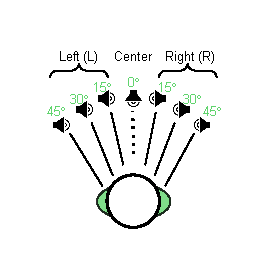
\includegraphics[scale=1, trim=5mm 5mm 5mm 5mm, clip]
        {../bth_perceptual_test_panned_speech/speech_angles.pdf}
      };
      \node at (6,0) {
        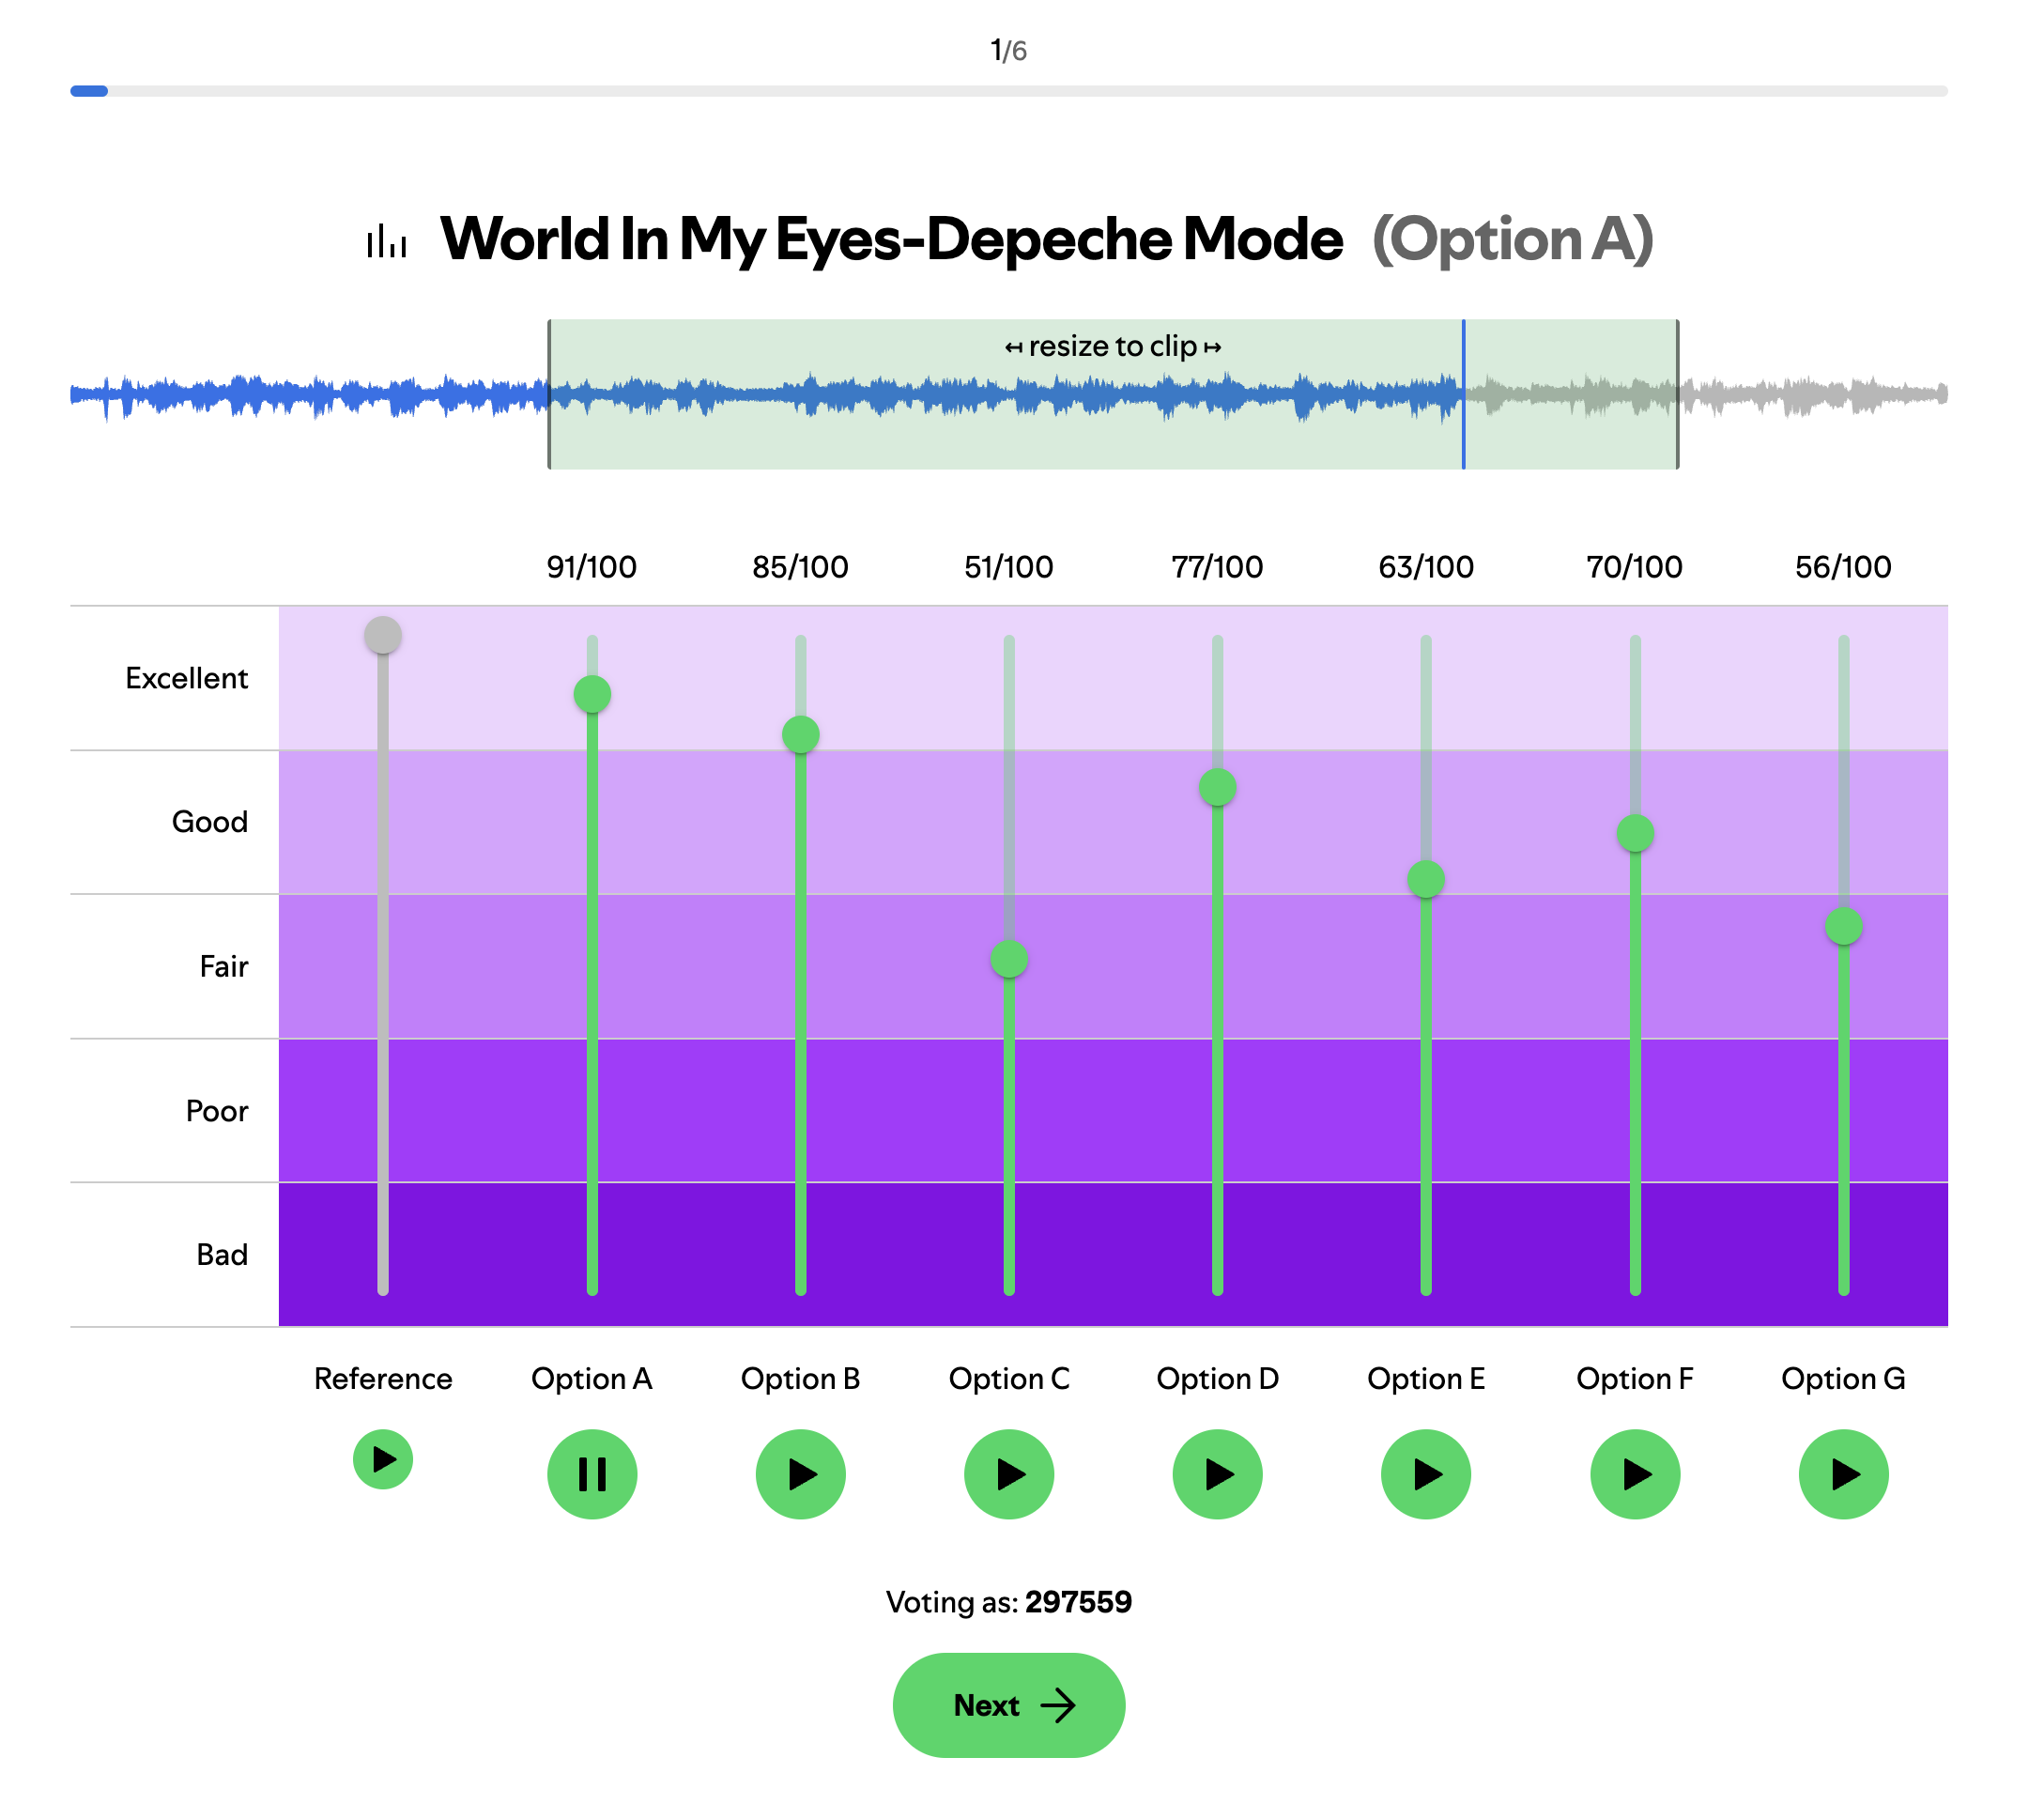
\includegraphics[scale=0.18]
        {../bth_perceptual_test_panned_speech/screenshot_cropped.png}
      };
    \end{tikzpicture}
  }
  \only<2> {
    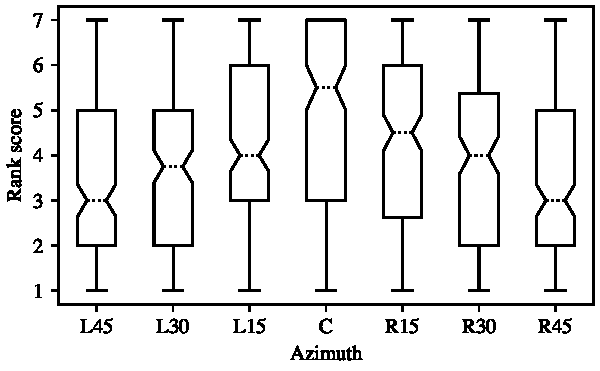
\includegraphics[height=0.7\textheight]{../../bth_jaes/rank_boxplots.pdf}
  }
  \\\parencite{miticPerceptualEvaluationBinaurally2026}
\end{frame}


\begin{frame}
  \paperslide
    {Paper IV}
    {miticPerceptualEvaluationBinaurally2026}
    {16cm}
    {../kappa/external_pages/Percept_Eval_Binaurally_Panned_Speech_Music_Mixtures.pdf}
    {People generally prefer centrally-panned speech but have highly personal preferences. Speech becomes the dominant audio source and is paramount to overall pleasantness.}
  \note{2026-10-27 - JAES sent it back for very minor revisions}
\end{frame}


\section{Discussion}

\subsection{Research questions}
\subsectionslide

\begin{frame}
  \frametitle{Research Questions and Answers}

  \begin{itemize}
    \item[\rqone:] How does the stereo image of a recording relate to real-world musical knowledge?
    \begin{itemize}
      \item Building a new musical instrument gave insight into what aspects of stereo field are noteworthy - (Paper I).
      \item Running existing SIP algorithms on lots of real music showcases what each one can detect - (Paper III)
      \item Stereo image might be used to maintain the perceptual quality of music when mixing it with other audio sources - (Paper IV).
    \end{itemize}
    \clearpage
    \item[\rqtwo:] What methods can be used to describe the stereo image of a music recording?
    \begin{itemize}
      \item Literal answer - (Paper II).
      \item What does each algorithm \q{hear}? - (Paper III).
    \end{itemize}
  \end{itemize}

\end{frame}

\subsection{Recurring themes}
\subsectionslide

\begin{frame}
  \frametitle{What is... Analysis {\tiny of stereo image in vast repositories of recorded music} ?}
  \begin{figure}
  \centering
  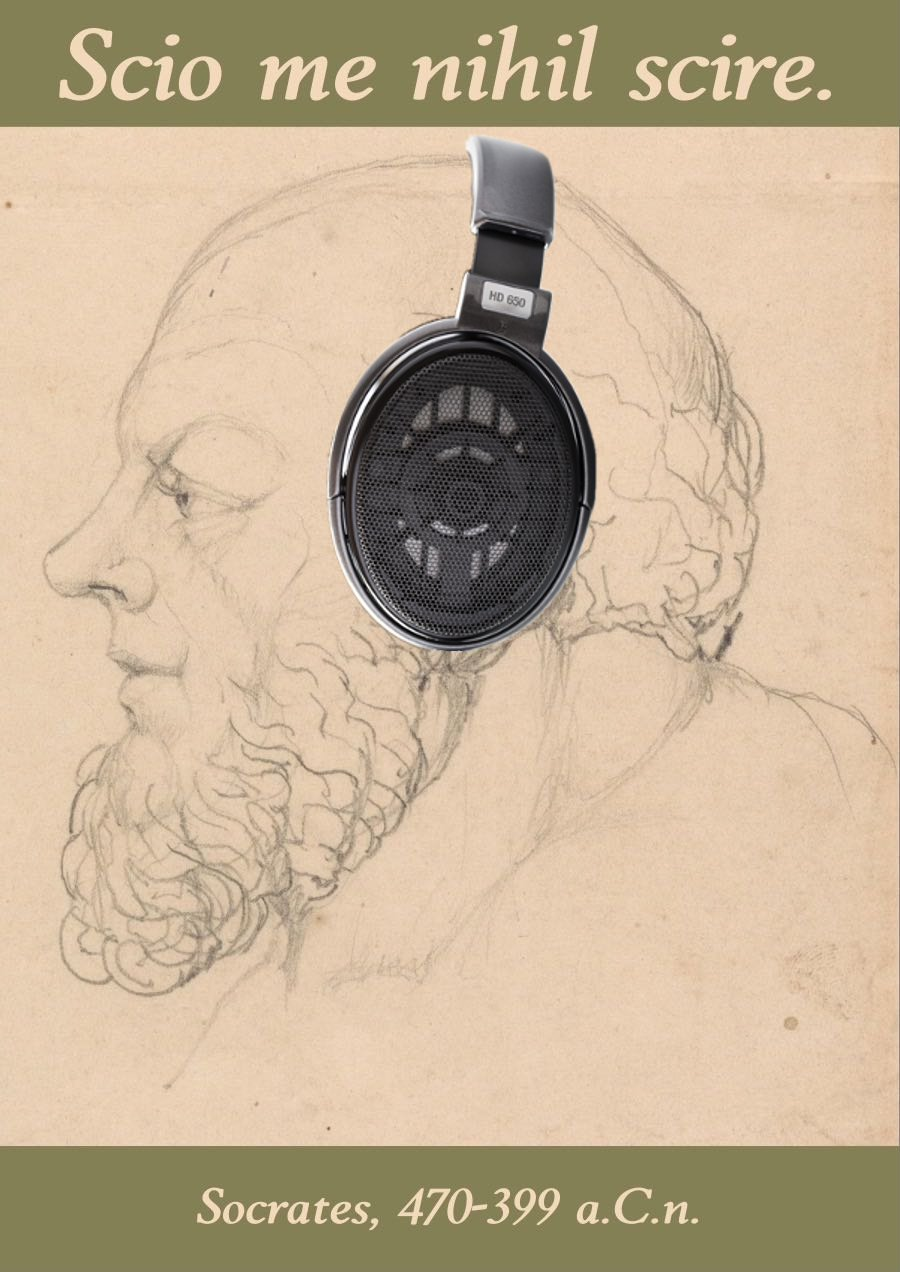
\includegraphics[height=0.8\textheight]{socrates_headphones.jpg}
  \end{figure}
  \note{Recurring theme - you can measure anything you want but there's no guarantee that it'll tell you what you want to know.}
\end{frame}

\begin{frame}
  \frametitle{Naming things is difficult}
  \centering
  \begin{tikzpicture}
    \node at (0,0) {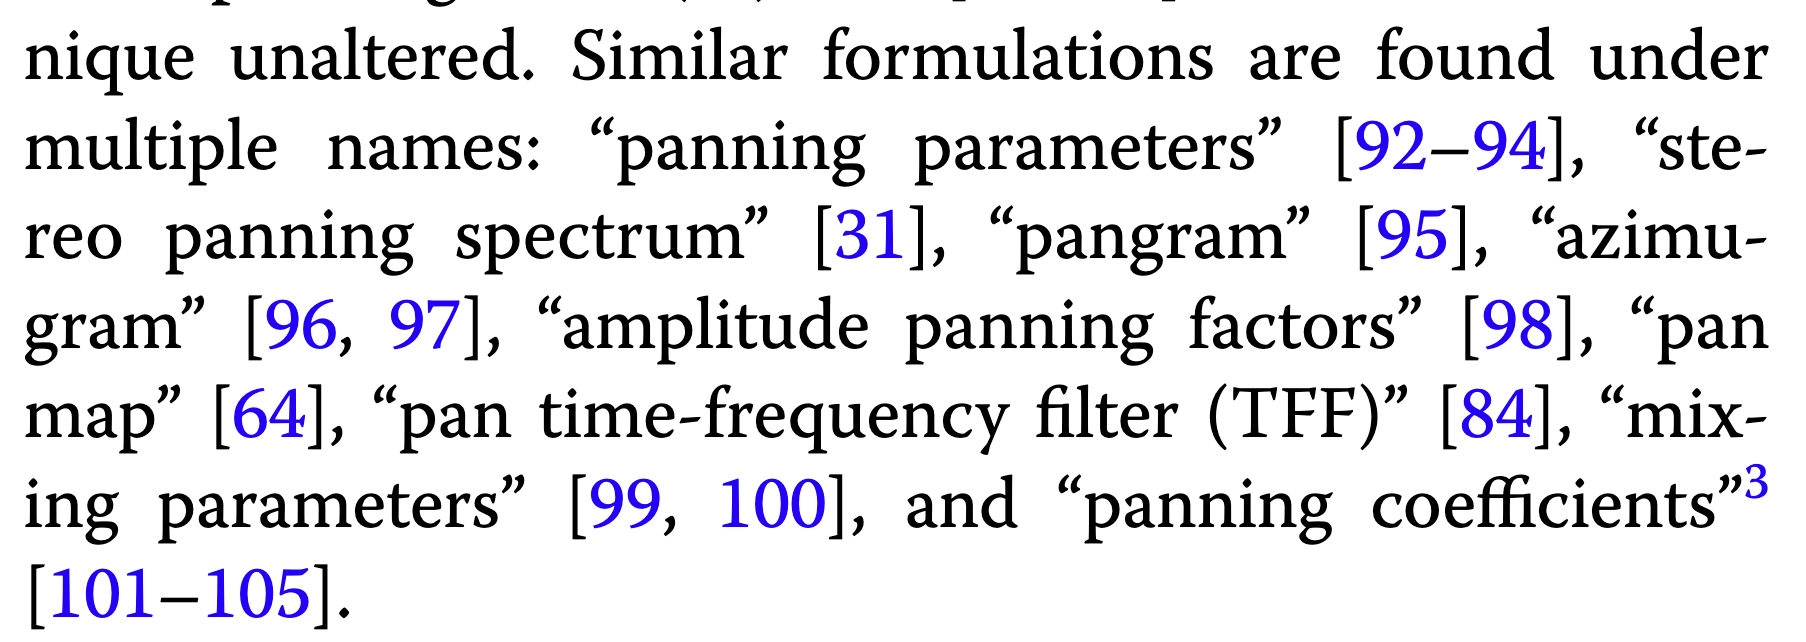
\includegraphics[width=0.4\textwidth]{naming_is_hard_1.png}};
    \node at (6,0.5) {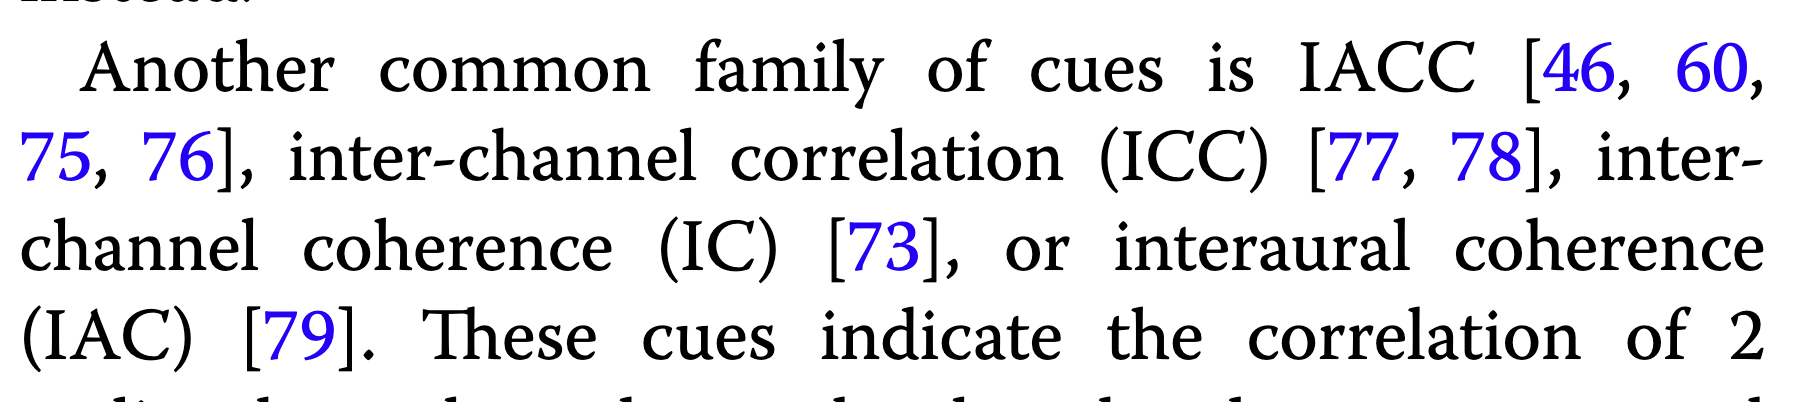
\includegraphics[width=0.4\textwidth]{naming_is_hard_3.png}};
    \node at (0,-2) {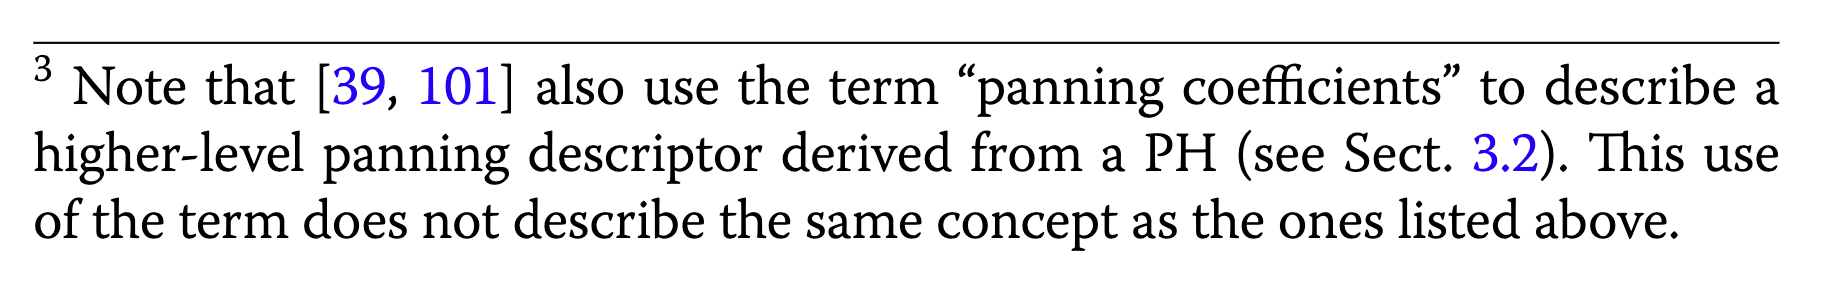
\includegraphics[width=0.4\textwidth]{naming_is_hard_2.png}};
    \node at (6,-2) {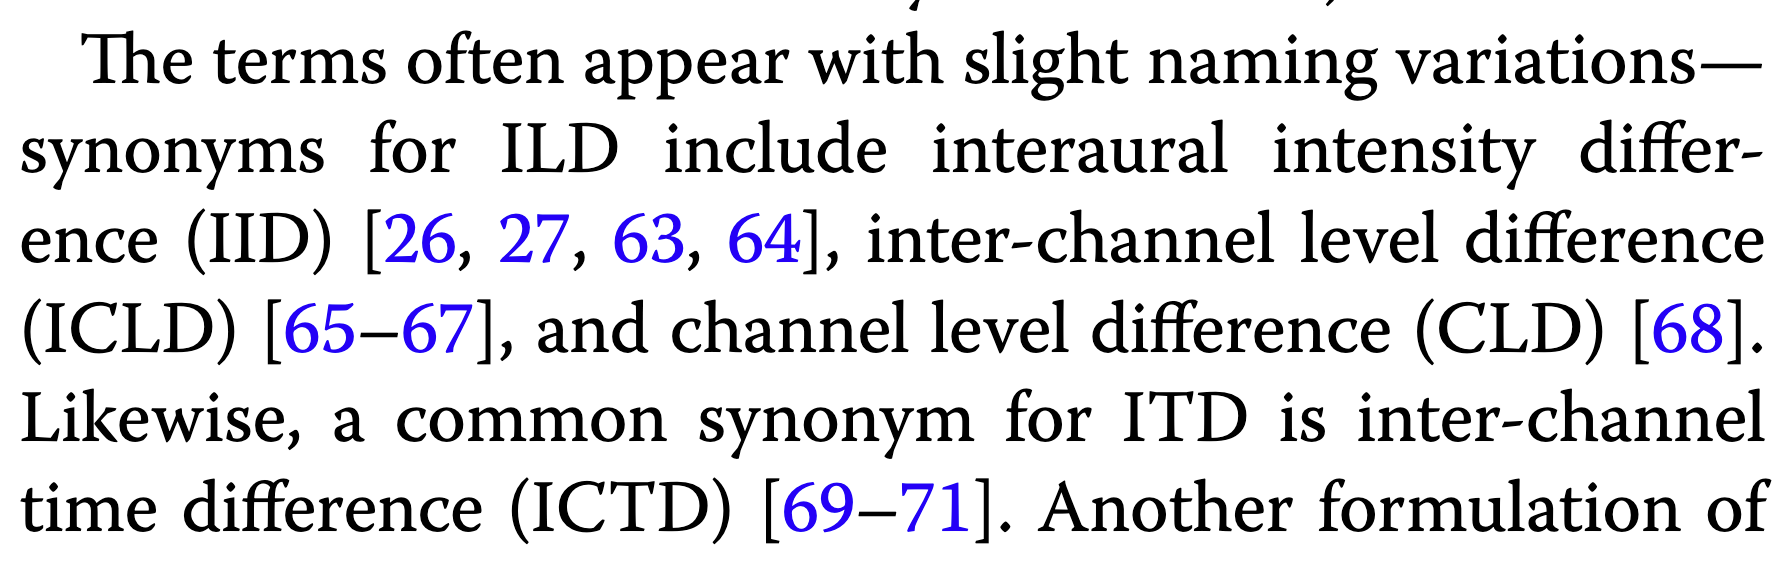
\includegraphics[width=0.4\textwidth]{naming_is_hard_4.png}};
  \end{tikzpicture}
  \\\parencite{miticSystematicLiteratureReview2026}
  \note{One of the reasons the SLR was so huge is that no one can agree on what anything is called.}
\end{frame}

\begin{frame}
  \frametitle{Computation is cheap}
  \begin{itemize}
    \setlength{\itemsep}{6pt}
    \item Theory-based DSP favoured over theory-free ML
    \item Could process everything on a laptop
    \item Access to music (not computing power) is the limitation 
  \end{itemize}
  \note{Spotify cost for processing about half a million files was about \$20. Idle cost for the machine was about \$1 per day.}
\end{frame}

\subsection{Limitations}
\subsectionslide

\begin{frame}
  \frametitle{Limitations}
  \begin{block}{Biases}
    \begin{itemize}
      \item All music and DSP algorithms are western
      \item Free music is a minority
    \end{itemize}
  \end{block}
  \begin{block}{Not covered}
    \begin{itemize}
      \item Overarching analysis of the global population of recordings
    \end{itemize}
  \end{block}
\end{frame}

\subsection{Future work}
\subsectionslide

\begin{frame}
  \frametitle{Future work}
  \begin{block}{Continuation to doctoral studies}
    \begin{itemize}
      \setlength{\itemsep}{6pt}
      \item Study the global population of music recordings
      \item Compare the content of disparate datasets
      \item Investigate distortions resulting from distribution
      \item Fully answer the overarching research question
    \end{itemize}
  \end{block}
\end{frame}

\section{Conclusion}

\begin{frame}
  \frametitle{Conclusion}
  \begin{itemize}
    \setlength{\itemsep}{6pt}
    \item Technological context and sonic content are inherently interconnected
    \item Stereo image descriptors exist, but are under-studied
    \item Measuring is easy - knowing what you measured is hard
  \end{itemize}
\end{frame}

\begin{frame}
  \frametitle{Questions?}
  \centering
  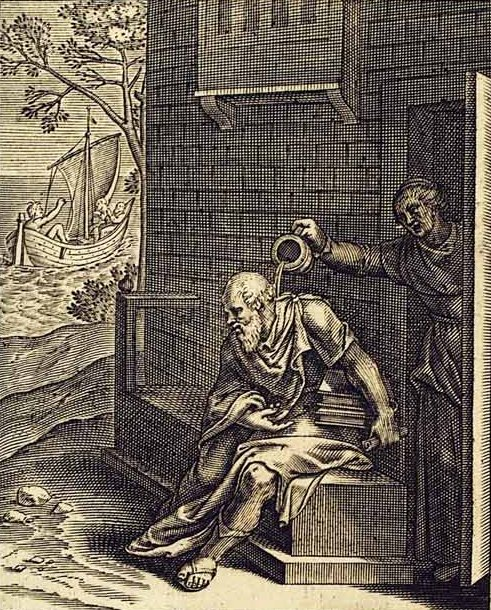
\includegraphics[height=0.8\textheight]{Socrates_and_Xanthippe.jpg}
  \note{Socrates and Xanthippe}
\end{frame}

\begin{frame}[allowframebreaks]
  \frametitle{References}
  \AtNextBibliography{\tiny} 
  \printbibliography
\end{frame}


\begin{frame}
  Here be dragons
\end{frame}


\end{document}